\documentclass[a4paper,12pt,twoside,openany]{book}

% \usepackage{fancyhdr}

% \pagestyle{fancy}
% \fancyhf{}
% \fancyhead[LE,RO]{Share\LaTeX}
% \fancyhead[RE,LO]{Guides and tutorials}
% \fancyfoot[CE,CO]{\leftmark}
% \fancyfoot[LE,RO]{\thepage}
% \usepackage{graphics} % for pdf, bitmapped graphics files
%\usepackage{mathptmx} % assumes new font selection scheme installed

\usepackage[linesnumbered,vlined,ruled]{algorithm2e}
\usepackage{amsmath, amssymb, bm}
\usepackage{amsthm}
\usepackage{array}
\usepackage{balance}
\usepackage[english]{babel}
\usepackage{color}
\usepackage{epsfig}
\usepackage{flushend}
\usepackage{fullpage}
\usepackage{graphics}
\usepackage{graphicx}
\usepackage{grffile}
\usepackage{helvet} % font sf = helvetica
\PassOptionsToPackage{hyphens}{url}\usepackage[bookmarks=true]{hyperref}
\usepackage[utf8]{inputenc}
% \usepackage[latin1]{inputenc}
\usepackage{listings}
\usepackage{minitoc}
\usepackage{multirow}
%\usepackage{mathptmx} % font = times
\usepackage[square,sort,comma]{natbib}
\usepackage{outlines}
\usepackage{pdfpages}
\usepackage{relsize}
\usepackage[figuresright]{rotating}
\usepackage{subcaption}
\usepackage{sidecap}
\usepackage{syntax}
\usepackage{titlesec}
\usepackage{url}
\usepackage{verbatim}
\usepackage{xspace}
\usepackage{tikz}
\usepackage{times} % assumes new font selection scheme installed
%\usetikzlibrary{arrows,shapes}
\setcounter{secnumdepth}{4}

%\titleformat{\paragraph}
%{\normalfont\normalsize\bfseries}{\theparagraph}{1em}{}
%\titlespacing*{\paragraph}
%{0pt}{3.25ex plus 1ex minus .2ex}{1.5ex plus .2ex}


\theoremstyle{definition}
\newtheorem{definition}{Definition}[section]
 
\theoremstyle{remark}
\newtheorem*{remark}{Remark}
 
\newcommand{\fig}[1]{Fig.~\ref{#1}}
\newcommand{\tbl}[1]{Table~\ref{#1}}
\newcommand{\algo}[1]{Algorithm~\ref{#1}}
\newcommand{\sect}[1]{Sec.~\ref{#1}}
\newcommand{\chapt}[1]{Chapter ~\ref{#1}}
\newcommand{\etal}[0]{{\em et al.~}}
\newcommand{\eg}[0]{{\em e.g.,~}}
\newcommand{\ie}[0]{{\em i.e.,~}}
\newcommand{\etc}[0]{{\em etc.\xspace}}
\newcommand{\myparagraph}[1]{\vspace{1mm} \noindent \textbf{#1}}
\newcommand{\comments}[2]{{\small{\textcolor[rgb]{0.0, 0.5, 0.0}{#2}}--[\textsc{#1}]}}
\newcommand{\note}[1]{{{\textcolor[rgb]{0.4, 0.4, 0.4}{\em #1}}}}
\newcommand{\todo}[1]{{{\textcolor[rgb]{0.9, 0.4, 0.4}{TODO: \em #1}}}}
\newcommand{\camera}[1]{{#1}}
\newcommand\abstractname{Abstract}
%%% BEGIN DOCUMENT
\linespread{1.213}
\begin{document}
%% some details about the thesis
\title{This is the title of the thesis}
\author{Author's name}
\advisor{Advisor's name}

% about the degree
\degree{Doctor of Philosophy}
\field{Subject}
\degreeyear{Year}
\degreemonth{Month}

% about the university
\department{Department}
\university{Harvard University}
\universitycity{Cambridge}
\universitystate{Massachusetts}
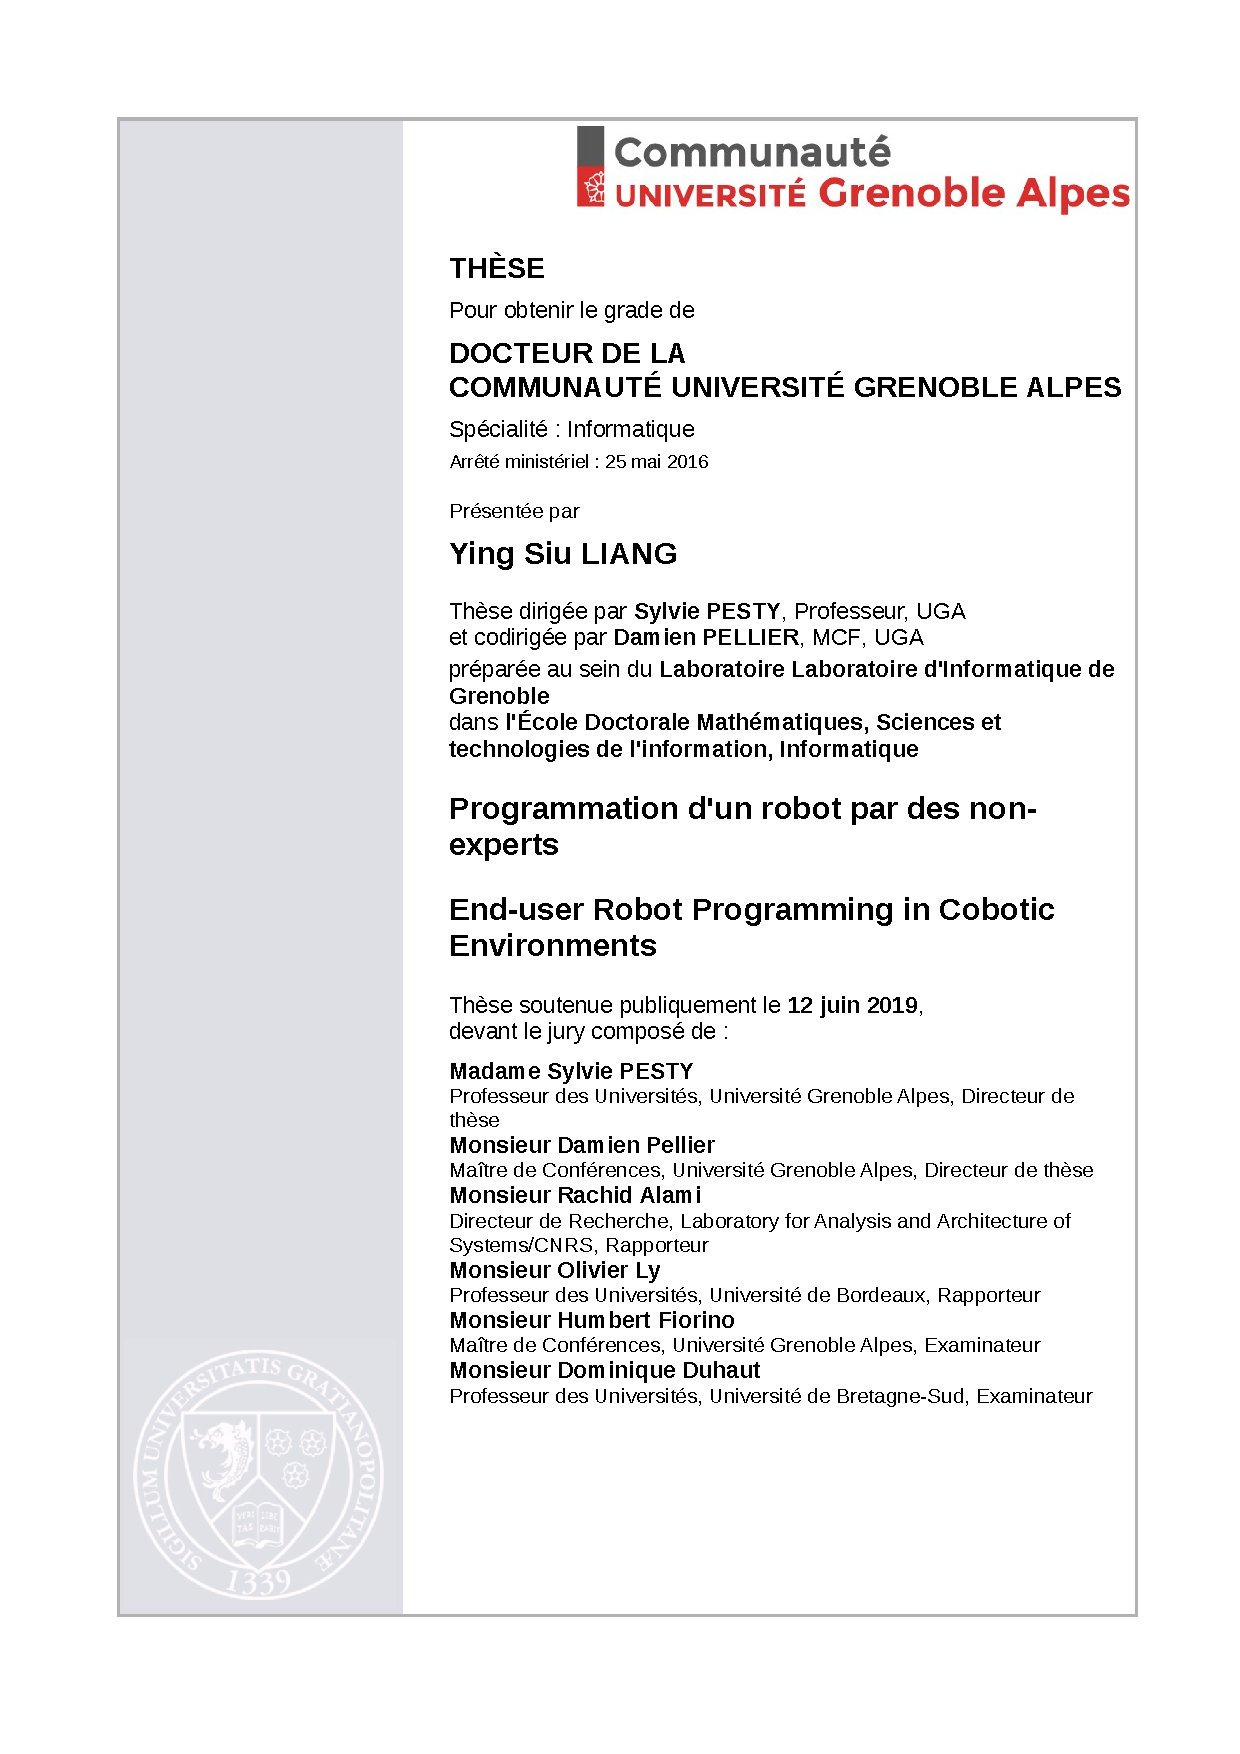
\includepdf[pages=1-1]{0-frontmatter/couverture.pdf}
% \maketitle
% \copyrightpage
% \abstractpage

%\chapter*{Contenu du rapport \`{a} mi-parcours}
%Le rapport à mi-parcours contient
\begin{itemize}
\item un calendrier prévisionnel précis et réaliste pour la troisième année et jusqu’à la soutenance de la thèse,
\item un CV (liste de publications, responsabilités, enseignement,…),
\item un bilan des formations suivies et prévues (extrait du compte personnel ADUM),
\item rapport à mi-parcours (y compris l'état de l'art, reprise des 2+1 articles accompagnés d'une présentation générale).
\end{itemize}

\section*{Calendrier prévisionnel pour la troisième année}
Date de la 1ere inscription en thèse: 28 octobre 2016\\
Date de soutenance prévue: septembre 2019\\

\begin{table}[ht]
\begin{center}
\begin{tabular}{r|c|c}
Dates & Task & Details\\ \hline
Aug`18 & Finish implementation work & Complete end-to-end system\\
Sep`18 & First evaluation/experiments & User studies with end-to-end system\\
Oct`18 &Improve framework based on first experiments & Adjust program flow \\
Nov`18 & Second evaluation/experiments & User studies with improved system\\
Dec`18 & \textit{Buffer month} & Finish all experiments and evaluations\\
 & & Write paper for IJCAI`19\\ \hline
Jan`19 & Start full-time thesis write-up & Thesis state is 30\% of content \\
Feb`19 & 1st draft (to be reviewed by supervisors) & $\geq 60\%$ + add more content \\
Mar`19 & 2nd draft & $\geq80\%$ + structural changes \\
Apr`19 & 3rd draft & $\geq 90\%$ + structural changes only \\
May`19 & Final draft & Make final edits/modifications\\
 & Hand in thesis & Final submission of thesis to the jury\\
Sep`19 & \textbf{Thesis defence} & \\
\end{tabular}
\end{center}
\end{table}

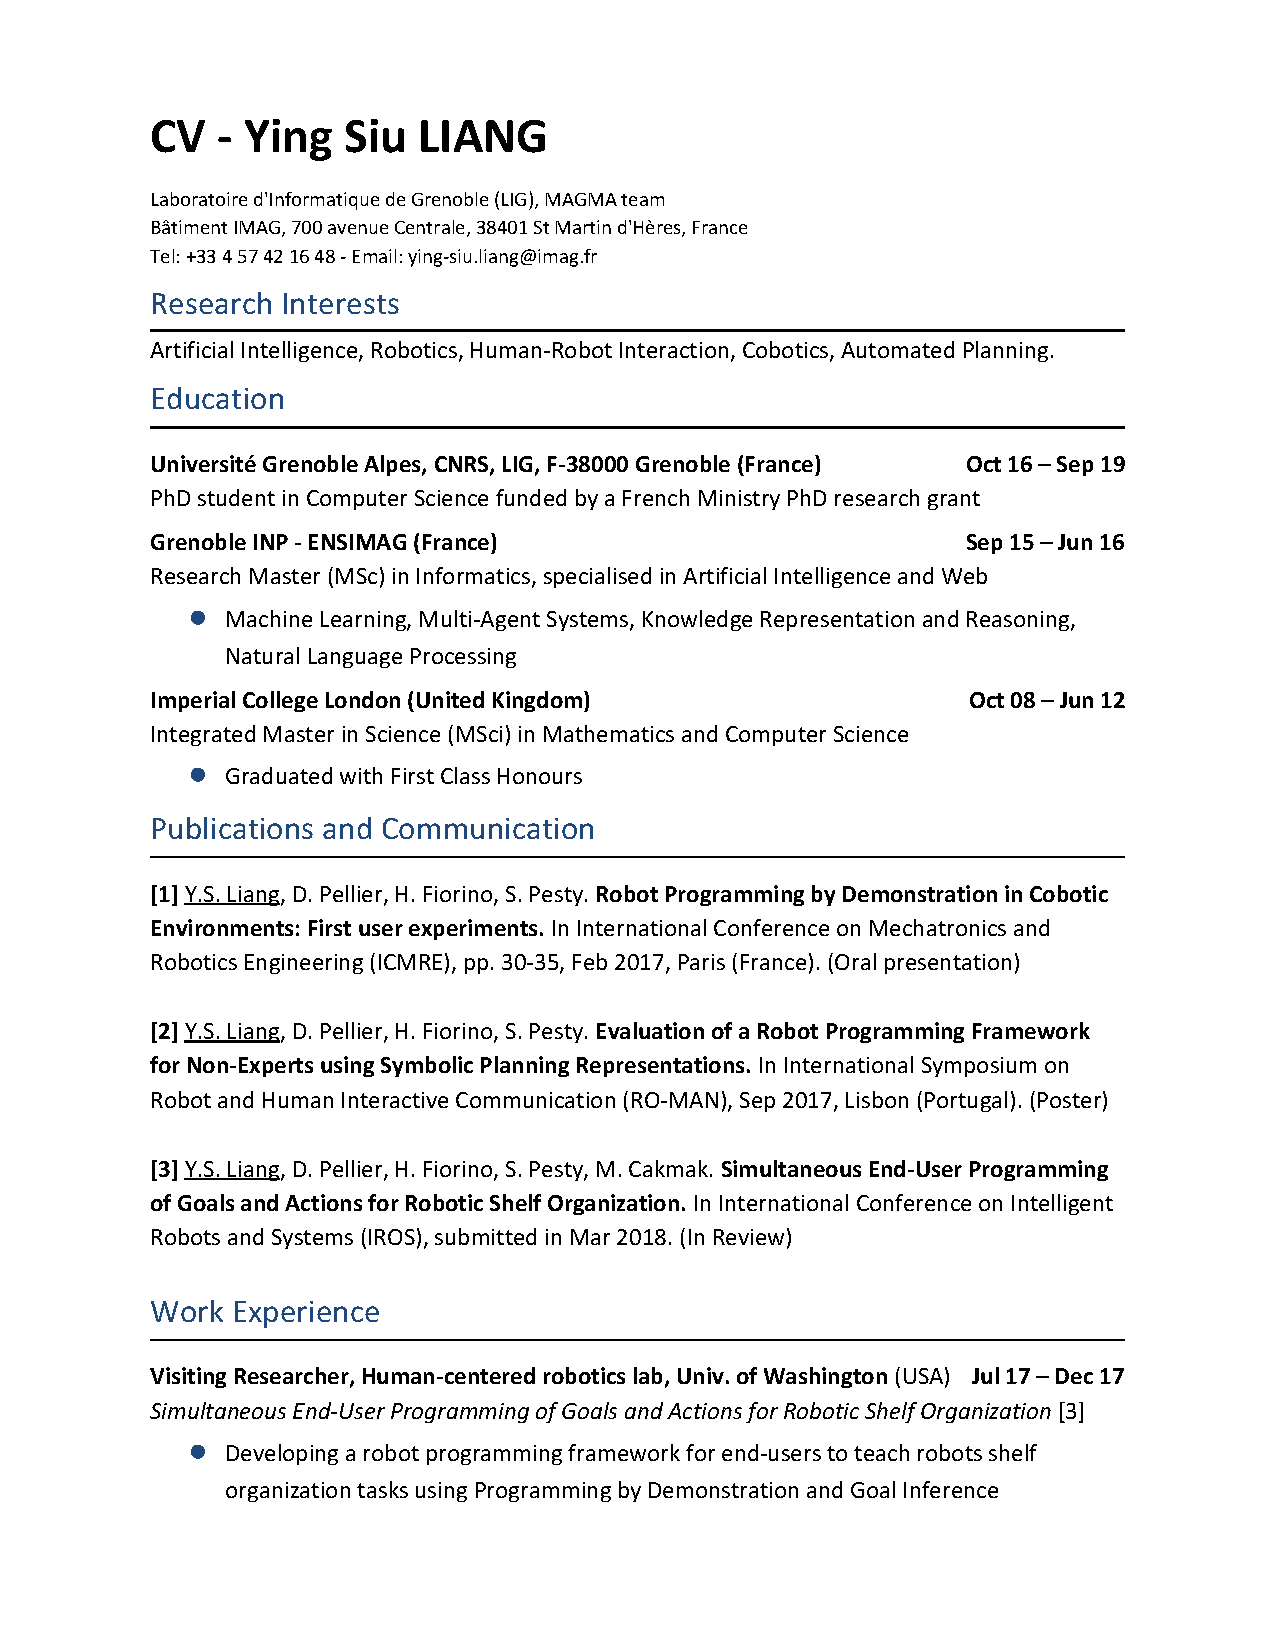
\includepdf[pages=1-2]{0-frontmatter/CV.pdf}
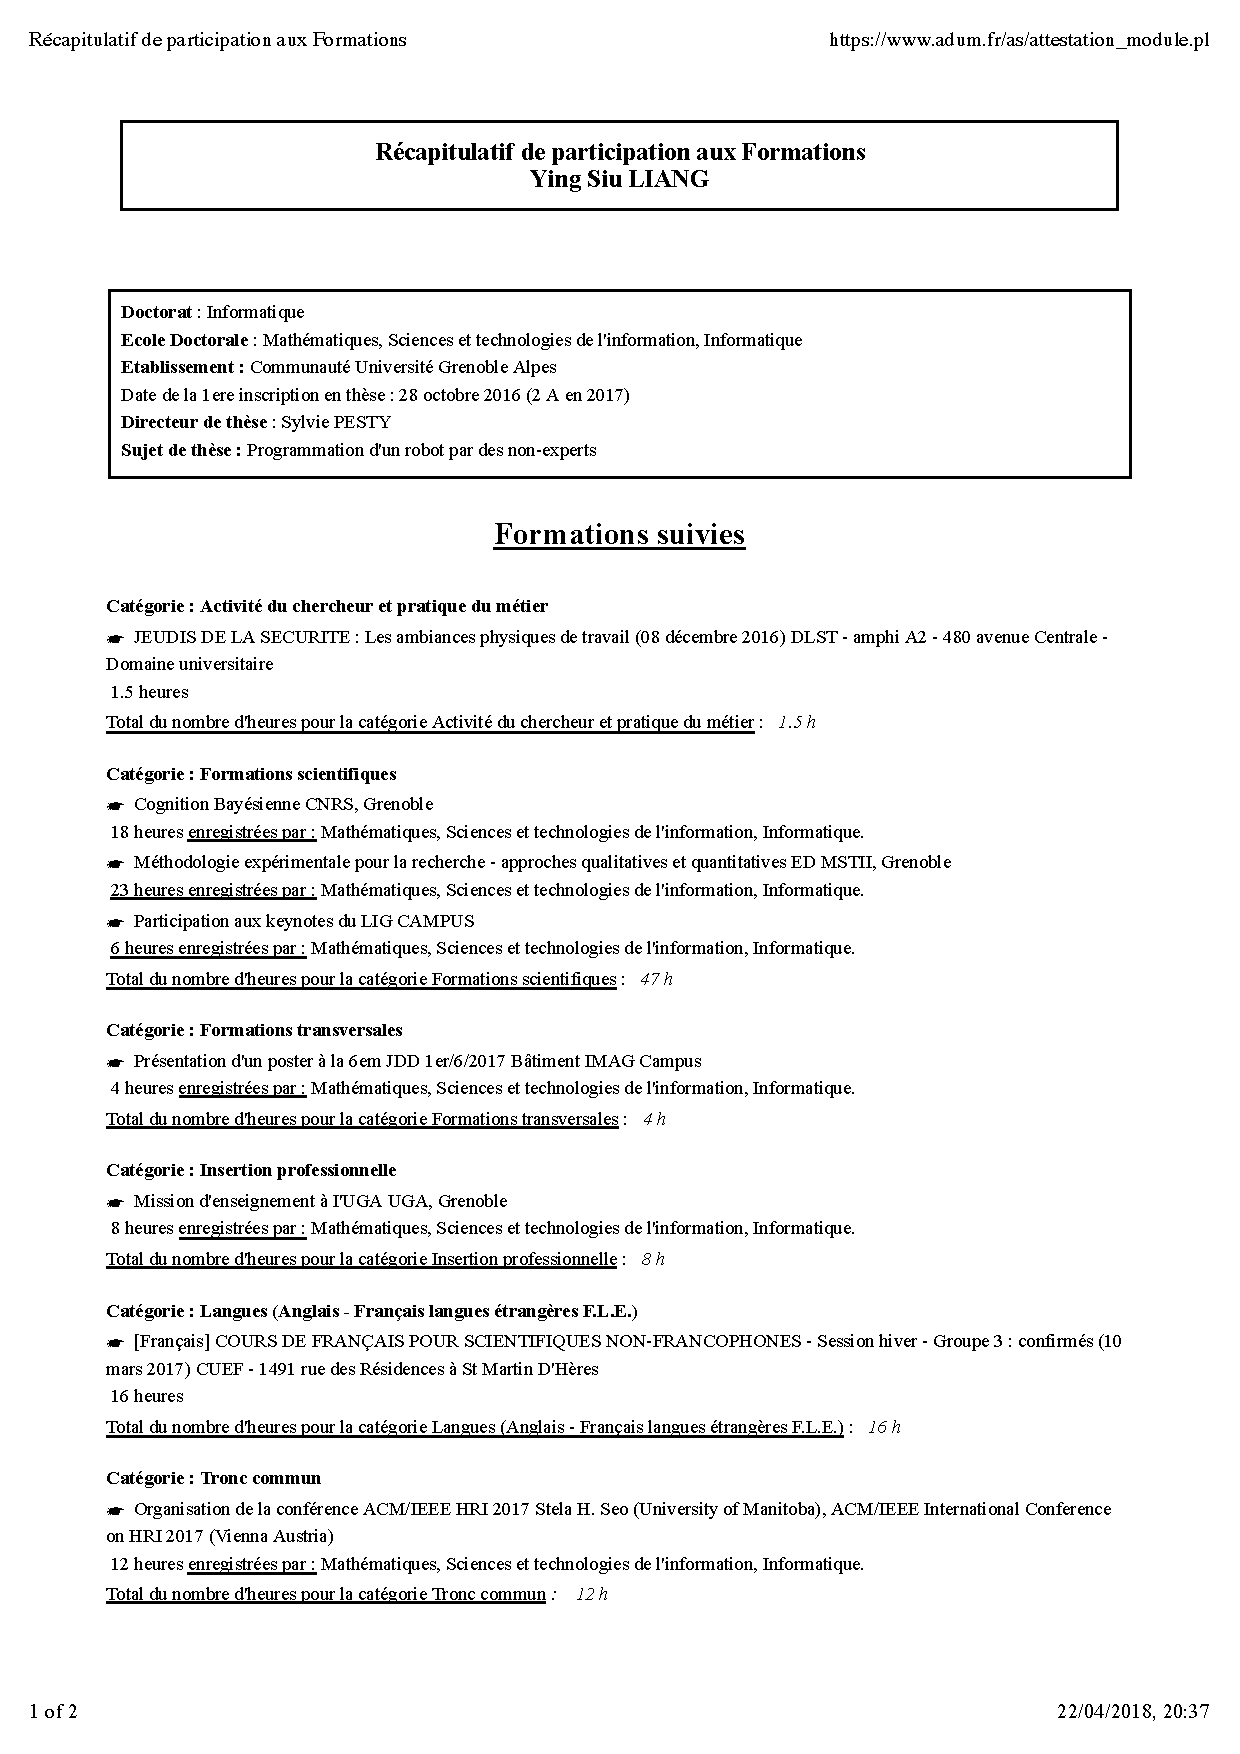
\includepdf[pages=1-2]{0-frontmatter/validated-credits.pdf}

\cleardoublepage
\chapter*{Abstract}
The increasing presence of robots in industries has not gone unnoticed. 
Cobots (collaborative robots) are revolutionising industries by allowing robots to work in close collaboration with humans.
Large industrial players have incorporated them into their production lines, but smaller companies hesitate due to high initial costs and the lack of programming expertise. 
In this thesis we introduce a framework that combines two disciplines, Programming by Demonstration and Automated Planning, to allow users without programming knowledge to program a robot. 
The user constructs the robot's knowledge base by teaching it new actions by demonstration, and associates their semantic meaning to enable the robot to reason about them. 
The robot adopts a goal-oriented behaviour by using automated planning techniques, where users teach action models expressed in a symbolic planning language (PDDL).

In this thesis we present preliminary work on user experiments using a Baxter Research Robot to evaluate our approach.
We conducted qualitative user experiments to evaluate the user's understanding of the symbolic planning language and the usability of the framework's programming process.
We showed that users with little to no programming experience can adopt the symbolic planning language, and use the framework.

We further present our work on a Programming by Demonstration system used for organisation tasks.
The system includes a goal inference model to accelerate the programming process by predicting the user's intended product configuration.

\paragraph{Keywords:} Robotics, Cobotics, End-User Programming, Programming by Demonstration, Automated Planning

\chapter*{R\'{e}sum\'{e}}
La présence croissante des robots dans les industries n'est pas passée inaperçue. 
Les cobots (robots collaboratifs) révolutionnent les industries en permettant aux robots de travailler en collaboration avec l'homme.
Les grands acteurs industriels les ont intégrés dans leurs chaînes de production, mais les petites entreprises hésitent en raison des coûts initiaux élevés et surtout du manque d'expertise en programmation. 
Les travaux récents se sont concentrés sur la possibilité pour les utilisateurs finaux de programmer des robots, mais apprendre des actions réutilisables est généralement laissé à des experts en robotique.
Dans cette thèse, nous proposons un système qui combine deux disciplines, la programmation par démonstration et la planification automatique, pour permettre à des utilisateurs ayant peu ou pas de connaissances techniques de programmer un robot. 
L'utilisateur construit la base de connaissances du robot en lui apprenant de nouvelles actions par démonstration, et associe leur signification sémantique via une interface graphique pour permettre au robot de raisonner à leur sujet. 
Le robot adopte un comportement orienté objectif en utilisant des techniques de planification automatisées pour réutiliser les actions apprises afin de générer des solutions pour des tâches inédites.
Nous présentons d'abord des travaux préliminaires en termes d'expériences d'utilisation à l'aide d'un robot de recherche Baxter pour évaluer la faisabilité de notre approche.
Nous avons mené des expériences qualitatives auprès des utilisateurs afin d'évaluer leur compréhension du langage de planification symbolique et de la convivialité du processus de programmation du système proposé.
Nous avons montré que les utilisateurs ayant peu ou pas d'expérience en programmation peuvent adopter le langage de planification symbolique et comprendre le processus de programmation proposé.
Nous présentons ensuite un système de programmation orienté objectif pour les tâches d'organisation robotique d'étagères qui utilise la programmation par démonstration pour enseigner simultanément les objectifs et les actions.
Sur la base des résultats obtenus et du système développé, nous présentons une implémentation d'iRoPro, un système fonctionnel de bout en bout qui permet d'enseigner des actions de bas et haut niveau par démonstration à réutiliser avec un planificateur de tâches.
Nous évaluons le pouvoir de généralisation du système et montrons comment les actions enseignées peuvent être réutilisées pour des tâches plus complexes.
Enfin, nous avons validé la convivialité du système par une étude d'utilisateurs et démontré que les utilisateurs de tous niveaux de programmation et de formation peuvent facilement apprendre et utiliser notre système de programmation de robot.

%\textbf{Mots-clés:} Robotique, Cobotique, Programmation utilisateur final, Programmation par démonstration, Planification automatisée

%Mots-clés : Robotique, Cobotique, Programmation utilisateur final, Programmation par démonstration, Planification automatisée 
\chapter*{Acknowledgements}
% parents
First of all, I would like to thank my parents P.Y. and H.K. Liang for the love, guidance and support they have shown me in every step of my life.
I would also like to thank my brother Chuen Tschi and other family members for being there for me when I needed.

Thanks to my thesis advisors Damien Pellier, Humbert Fiorino, and Prof. Sylvie Pesty for their supervision and guidance, as well as my former and current colleagues in the HAwAI (formerly MAGMA) team for their support throughout the thesis.
My sincere gratitude also goes to Nadine Mandran, who was always happy to help me with my user experiments and provided me with essential feedback on both the design and the write-up.
Similarly, I would like to thank other members of the lab and former interns that I worked with and that helped me with any aspects for my thesis.

% PhD advisor Pierre geneves 
I am also grateful to my advisor from école doctoral Dr. Pierre Genevès for providing an outside perspective and my external advisor Prof. Dominique Duhaut for believing in me.
I still remember the time when I just finished my Master thesis presentation in 2016, Dominique told me ``Someone like you should do a Ph.D." - and so I did.
Also thanks to the \textit{rapporteurs} Rachid Alami and Olivier Ly for their time and feedback to my thesis.

%Justin Huang
I would like to express my sincere gratitude to Maya Cakmak and the Human-Centered Robotics Lab, for inviting me to work with her for 5 months of my Ph.D.
%It was truly one of the most fun and inspiring experiences for me to continue work in robotics research after my thesis.
I would also like to thank my friends in Grenoble, Seattle, London, and anywhere else in the world who supported me throughout my thesis.
%Finally, I would like to thank my former boss John Hayes, who always asked me the unconventional question ``Is this really what you want to do?" and encouraged me to follow my interests which finally led to me doing this thesis.

%To the rest, \ie all people whose names start with a French alcoholic beverage, \eg vin, and end with a currency, \eg cent, I would like to NOT thank you for NOTHING because you simply suck.

\dominitoc% Initialization
\tableofcontents
%\authorlist
\listoffigures

%=====================

\chapter{Introduction} \label{chap:Intro}
\minitoc% Creating an actual minitoc
\section{Context}
% 1-2 pages max
Technologies have revolutionised the manufacturing industry ever since the Industrial revolution in the 19th century.
Robots are increasing productivity by replacing humans for arduous and repetitive manual tasks.
%are increasing productivity, efficiency, lower costs, and relieve humans from operationally dangerous tasks.
There is a noticeable increase in industrial robot order requests, as well as capital investments into the field.
Although robots can be superior in automating human tasks, there remain many that cannot be completely taken over and that still need human intervention, such as high-precision tasks.
To allow both human precision and robot automation, collaborative robots have been introduced.

\subsection{Cobotics}\label{subsec:Cobotics}
Collaborative robots, or \textit{cobots}, have been introduced by \cite{colgate1999cobots} and allow for a close collaboration between humans and robots.
They enable humans to perform tasks, which they cannot perform on their own, due to physical constraints such as the manipulation of heavy parts.
Furthermore, they reduce risks of work-related accidents, including health hazards such as exposure to dangerous environments (e.g. chemical acids, excessive temperatures or noise), as well as sleeping disorders caused by rotating work shifts.
Thus, cobots contribute to productivity gains as they are designed to take over manual and repetitive tasks and are able to respond to actions of the human operator.
While replacing jobs of low-skilled human workers, they open up a market for new high-skilled jobs.

Cobotic systems have been adopted in several industries from the food-processing industry (\cite{Food}), to aeronautics (\cite{Airbus}) to the health industry (\cite{Ebola}).
However, companies which resist the use of robots in their daily routines, consider the investment cost ineffective, due to their high initial costs and the lack of trained personnel.
%, who have the needed programming skills to fully operate and exploit the robots.
Traditional robot programming solutions require domain experts and robots are generally programmed to complete a specific task.
Recent approaches using large amounts of data (e.g. Neural Networks (\cite{billard2001robust})) or self-exploration (e.g. Reinforcement Learning (\cite{smart2002effective})) become infeasible for task-specific applications.
This is a bottleneck for industries as many robot programming solutions fail as the deployment in real world scenarios introduces further limitations. 
Thus, recent research has been focusing on robot programming for end-users.

\subsection{Robot Programming by Demonstration}
Robot Programming by Demonstration (PbD), also referred to as \textit{Learning from Demonstration}, is an end-user programming technique for teaching a robot new skills by demonstrating a task, without writing code (\cite{billard2008robot}).
Influenced by natural learning paradigms in humans and other animals, it is an intuitive robot programming method, with the goal to refine the robot's performance, by providing repetitive demonstrations.
PbD has become a central topic in research areas, with the aim to move from purely pre-programmed robots to flexible user-based interfaces for training robots.

Figure \ref{fig:Principle Overview} shows the life-cycle for teaching a robot by demonstration.
The teacher demonstrates the desired behaviour to the robot.
The robot uses its sensors for a multi-modal perception of the demonstration and extracts the relevant information to create a model of the skill.
The new skill is executed in a new context and evaluated by the teacher.
The teacher can refine the learned skill by providing additional demonstrations of the same skill.
The robot then generalises over the demonstrations by extracting relevant features that remained unchanged across the set of demonstrations.
This incremental learning process allows the robot to acquire a new skill from demonstrations provided by non-expert users.

\begin{figure}[h]
	\centering
	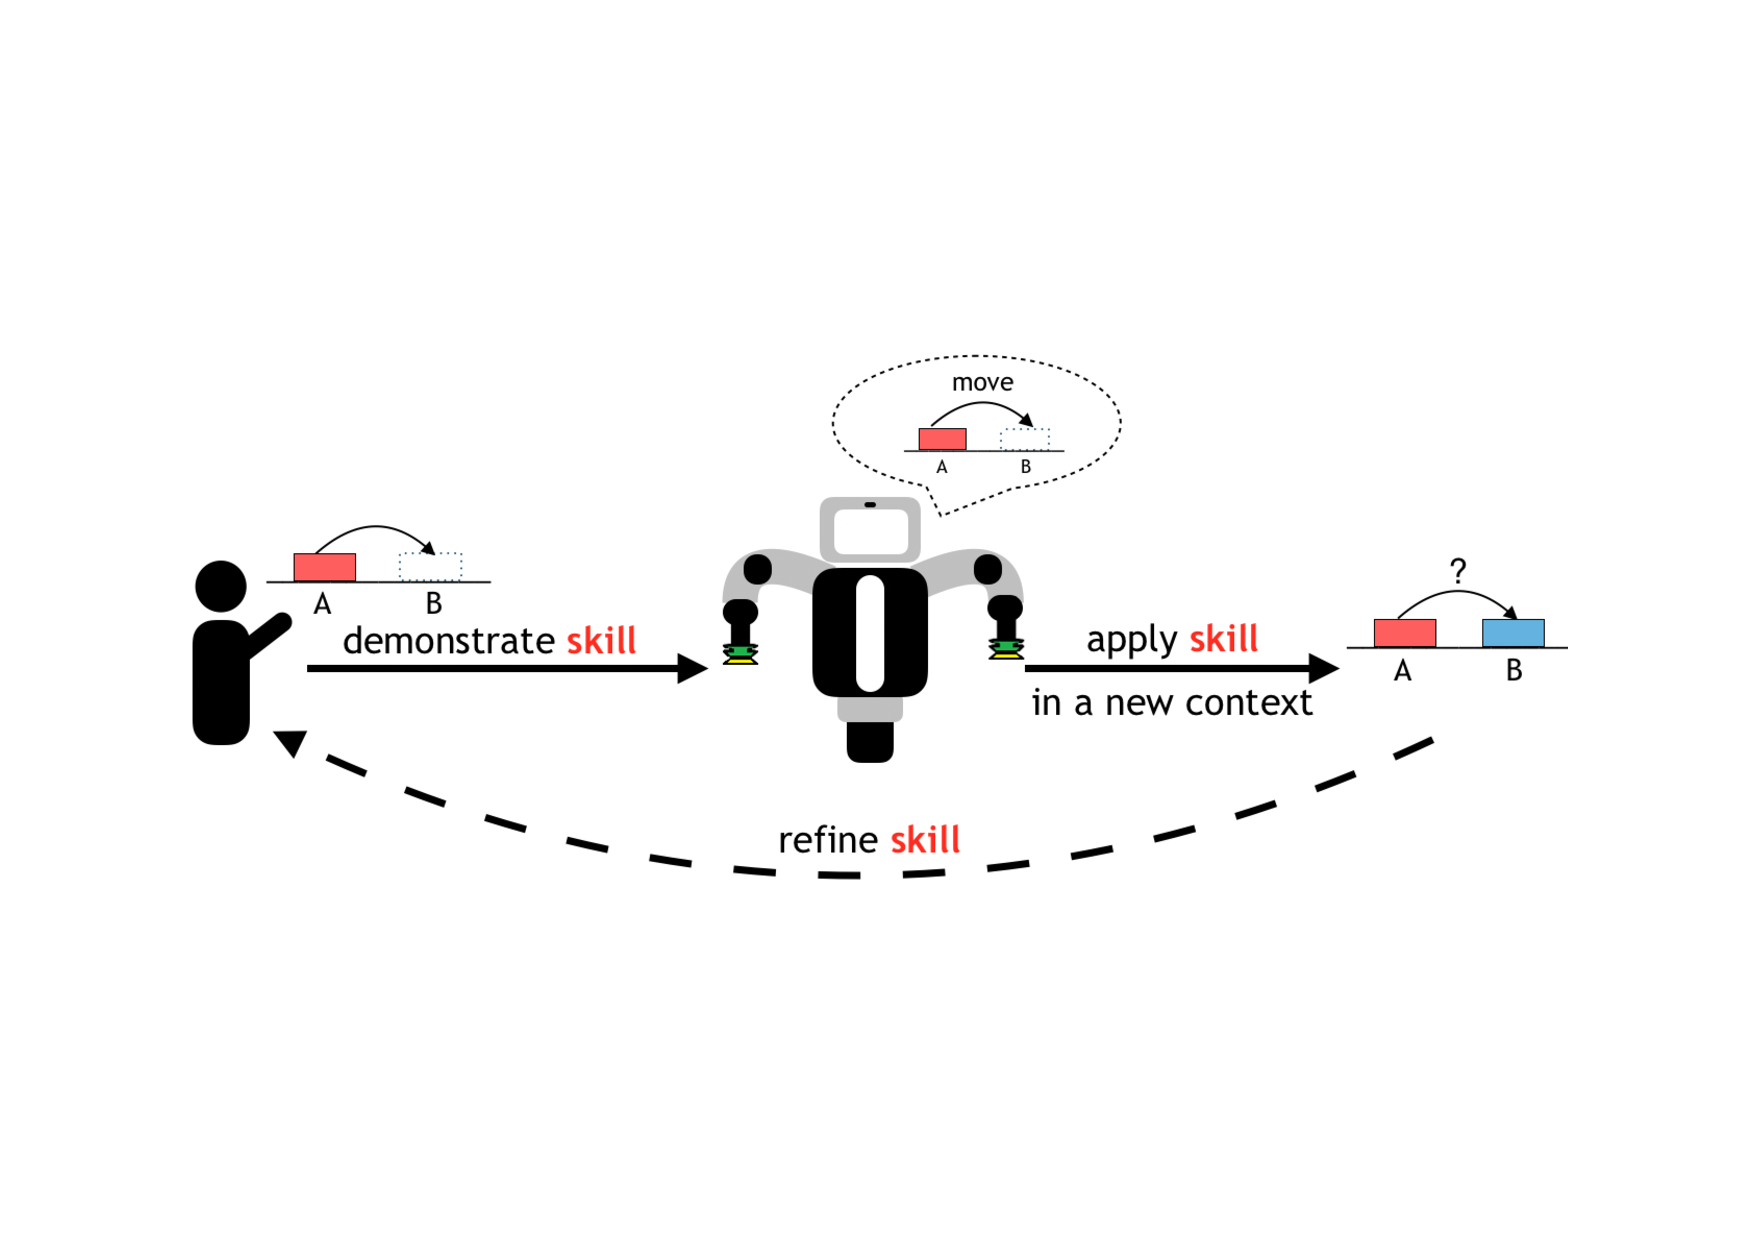
\includegraphics[width=0.5\linewidth]{figures/PbD-Overview}
	\caption{PbD Overview}
	\label{fig:Principle Overview}
\end{figure}

%Besides the advantage of being able to teach the robot tasks without the need to write code, PbD provides a powerful tool to improve learning abilities by reducing the search space of possible solutions.
However, learning object manipulation tasks is still considered a hard problem, as the robot has limited knowledge about the world and restricted sensor availability (\cite{ekvall2008robot}).
Many PbD algorithms have been proposed in the literature (\cite{argall2009survey,billing2010formalism}), but there still remain several challenges such as the suboptimality of demonstrations (\cite{chen2003programing,kaiser1995obtaining}) or the lack of comparative user studies (\cite{suay2012practical}).

% teaching full action sequences
Another major problem is that the robot is generally demonstrated an action sequence to complete a specific task (\cite{orendt2016robot,peppoloni2014ros}).
Take for example the Tower of Hanoi problem (\cite{douglas1985metamagical}) as shown in \fig{fig:Tower of Hanoi}a.
The objective is to move the entire stack to another rod, obeying the following simple rules:
\begin{itemize}
\item Only one disk can be moved at a time.
\item Each move consists of taking the upper disk from one of the stacks and placing it on top of another stack.
\item No disk may be placed on top of a smaller disk.
\end{itemize}

The robot can be taught an action sequence to solve the problem with three disks.
When the problem changes to four disks (\fig{fig:Tower of Hanoi}b), the robot has to be demonstrated a new sequence, even though both problems obey the same rules.
This is a complicated and time-consuming process and does not allow non-experts to reprogram robots for different tasks.
Ideally, we only teach the robot the objective and rules and let it generate the solution, or a \textit{plan}, on its own.

\begin{figure}[htp]
	\centering
	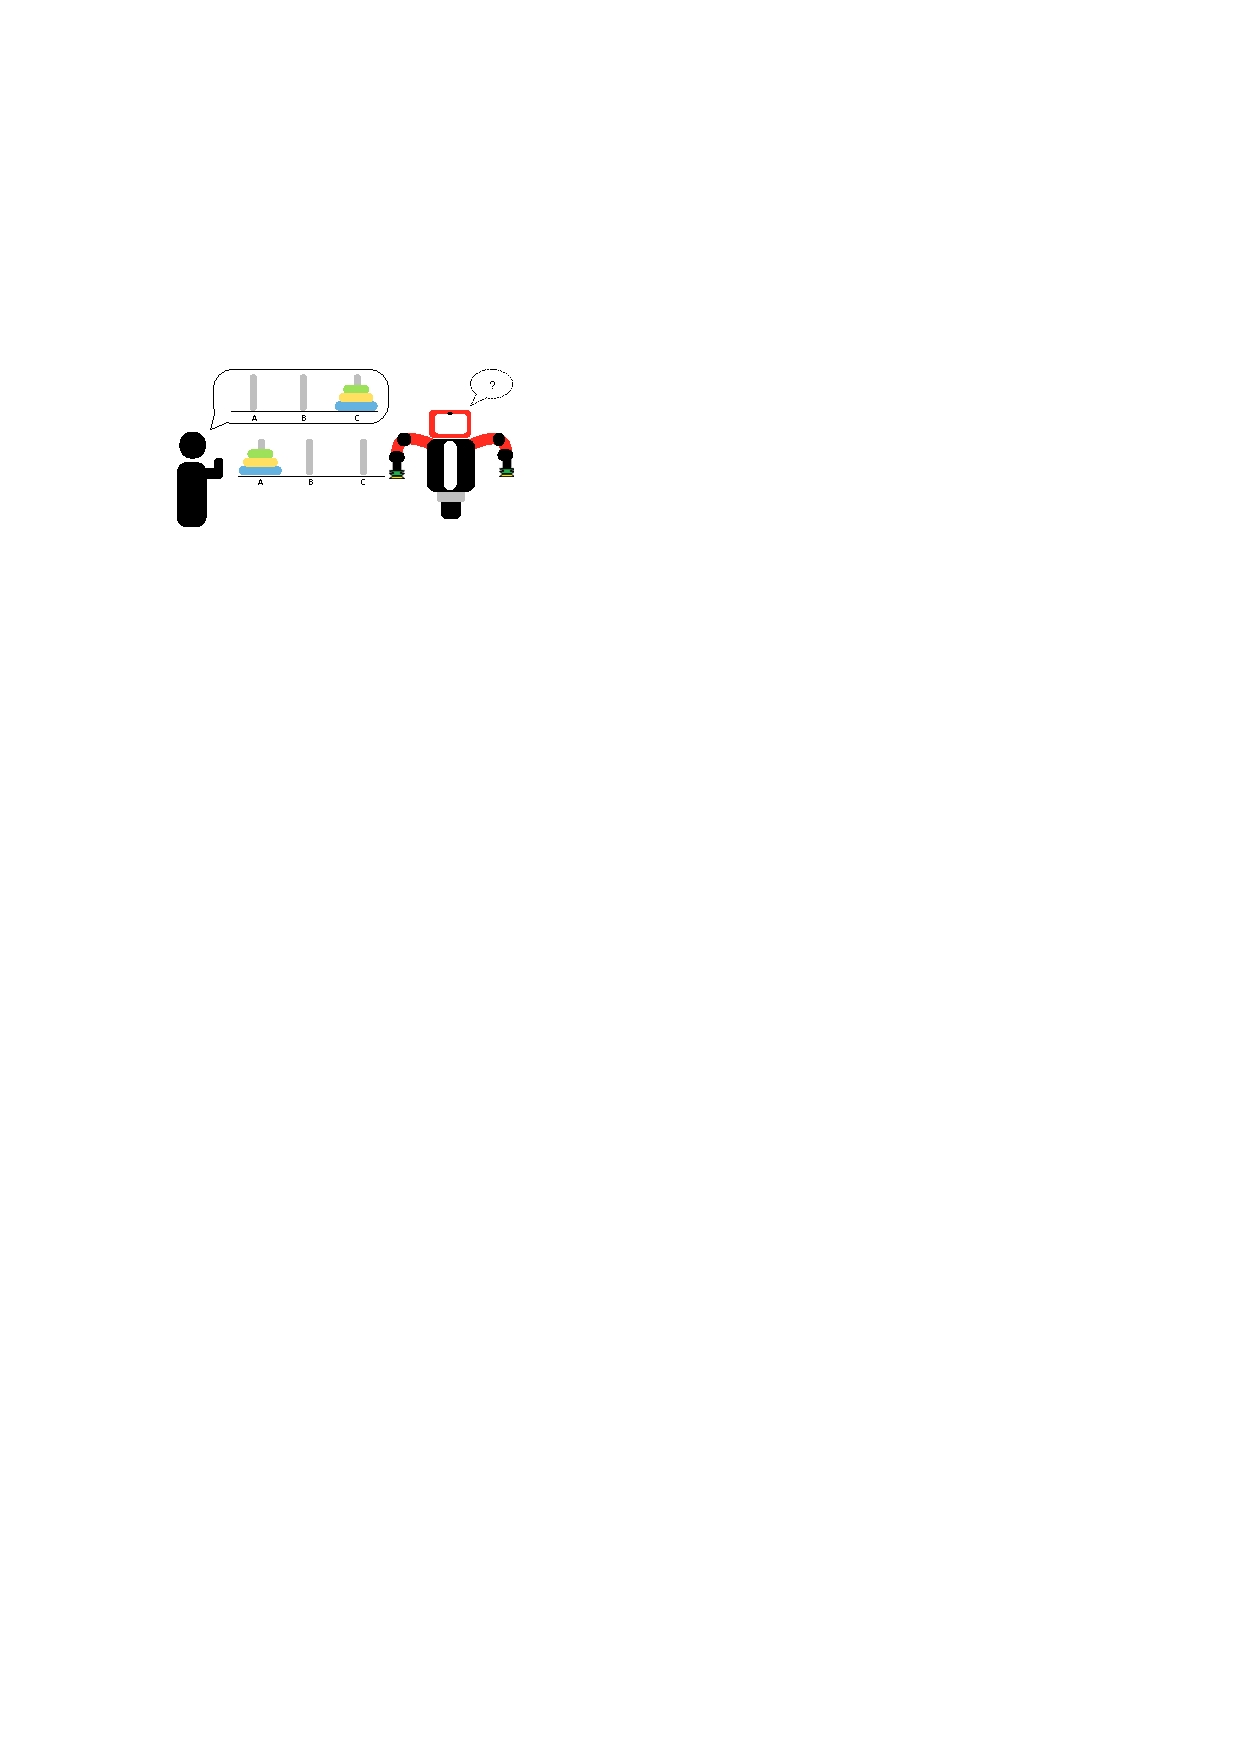
\includegraphics[width=.4\textwidth]{figures/hanoi-0}\hspace{2cm}%\hfill
	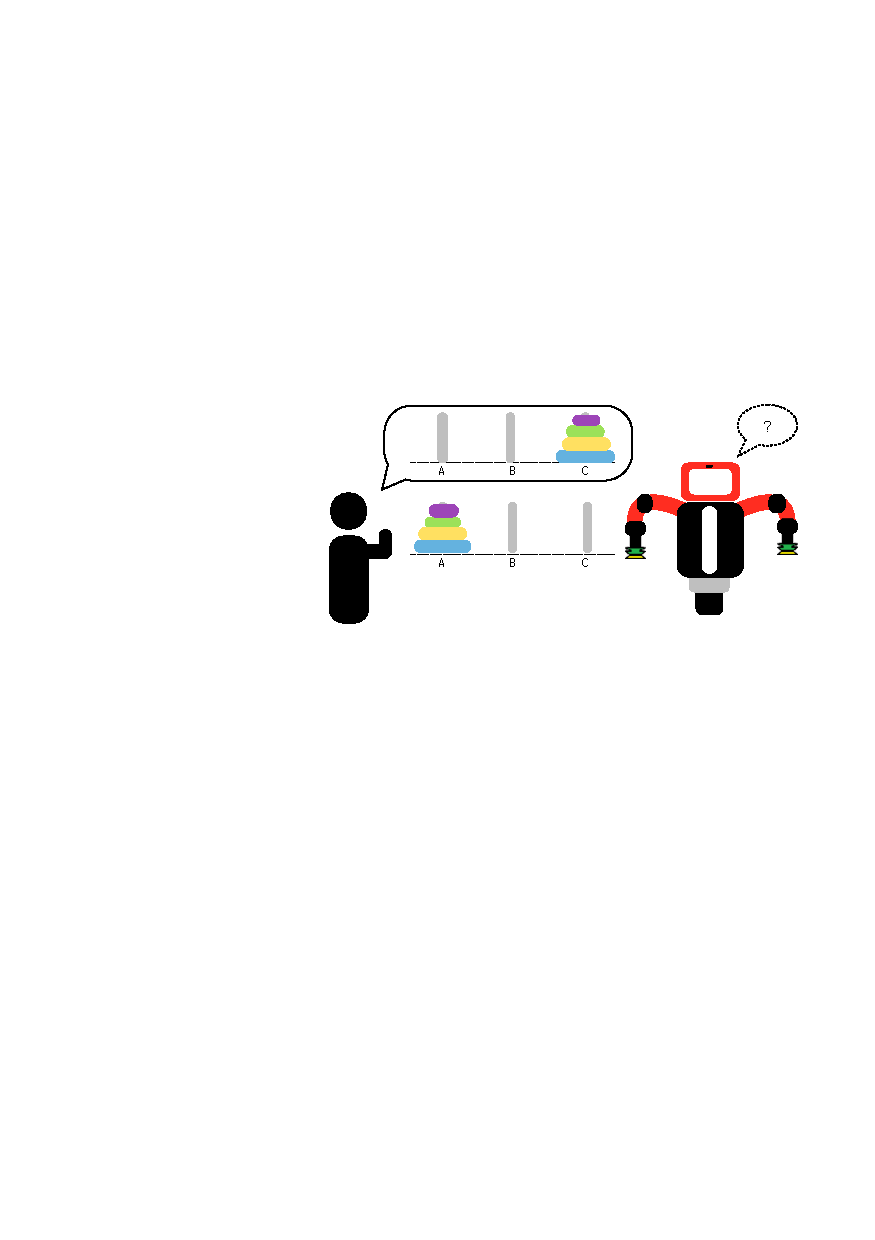
\includegraphics[width=.4\textwidth]{figures/hanoi-1}
	\caption{Tower of Hanoi problem a) with three disks b) with four disks}
	\label{fig:Tower of Hanoi}
\end{figure}

\subsection{Automated Planning}
Automated Planning, also known as \textit{AI Planning}, is a research field that focuses on the development of efficient search algorithms to generate solutions to problems.
Given a set of actions, a description of the state of the world, and some goal state, the planner generates a sequence of actions, which guarantees the transition from the initial state to the goal state (\fig{fig:Planning domain and action}).
To allow a correct transition between different states of the world, actions are defined in terms of preconditions and effects (\fig{fig:Planning domain and action}b). 
Planning algorithms use a symbolic planning language such as STRIPS (\cite{fikes1971strips}) or PDDL (\cite{ghallab2004automated}) as their standard encoding language.
The Tower of Hanoi problem could be defined as a planning problem and solved for any number of disks using an automated planner.
%In the initial state, the disks are stacked in ascending order (smallest at the top) on one of the pegs, in the goal state the disks are stacked in the same order on one of the other two remaining pegs. 
%The goal state must be achieved by obeying certain rules for moving the disks (e.g. only the top disk of a stack can be moved at a time and may not be placed on top of a smaller disk). 


\begin{figure}[htp]
	\centering
	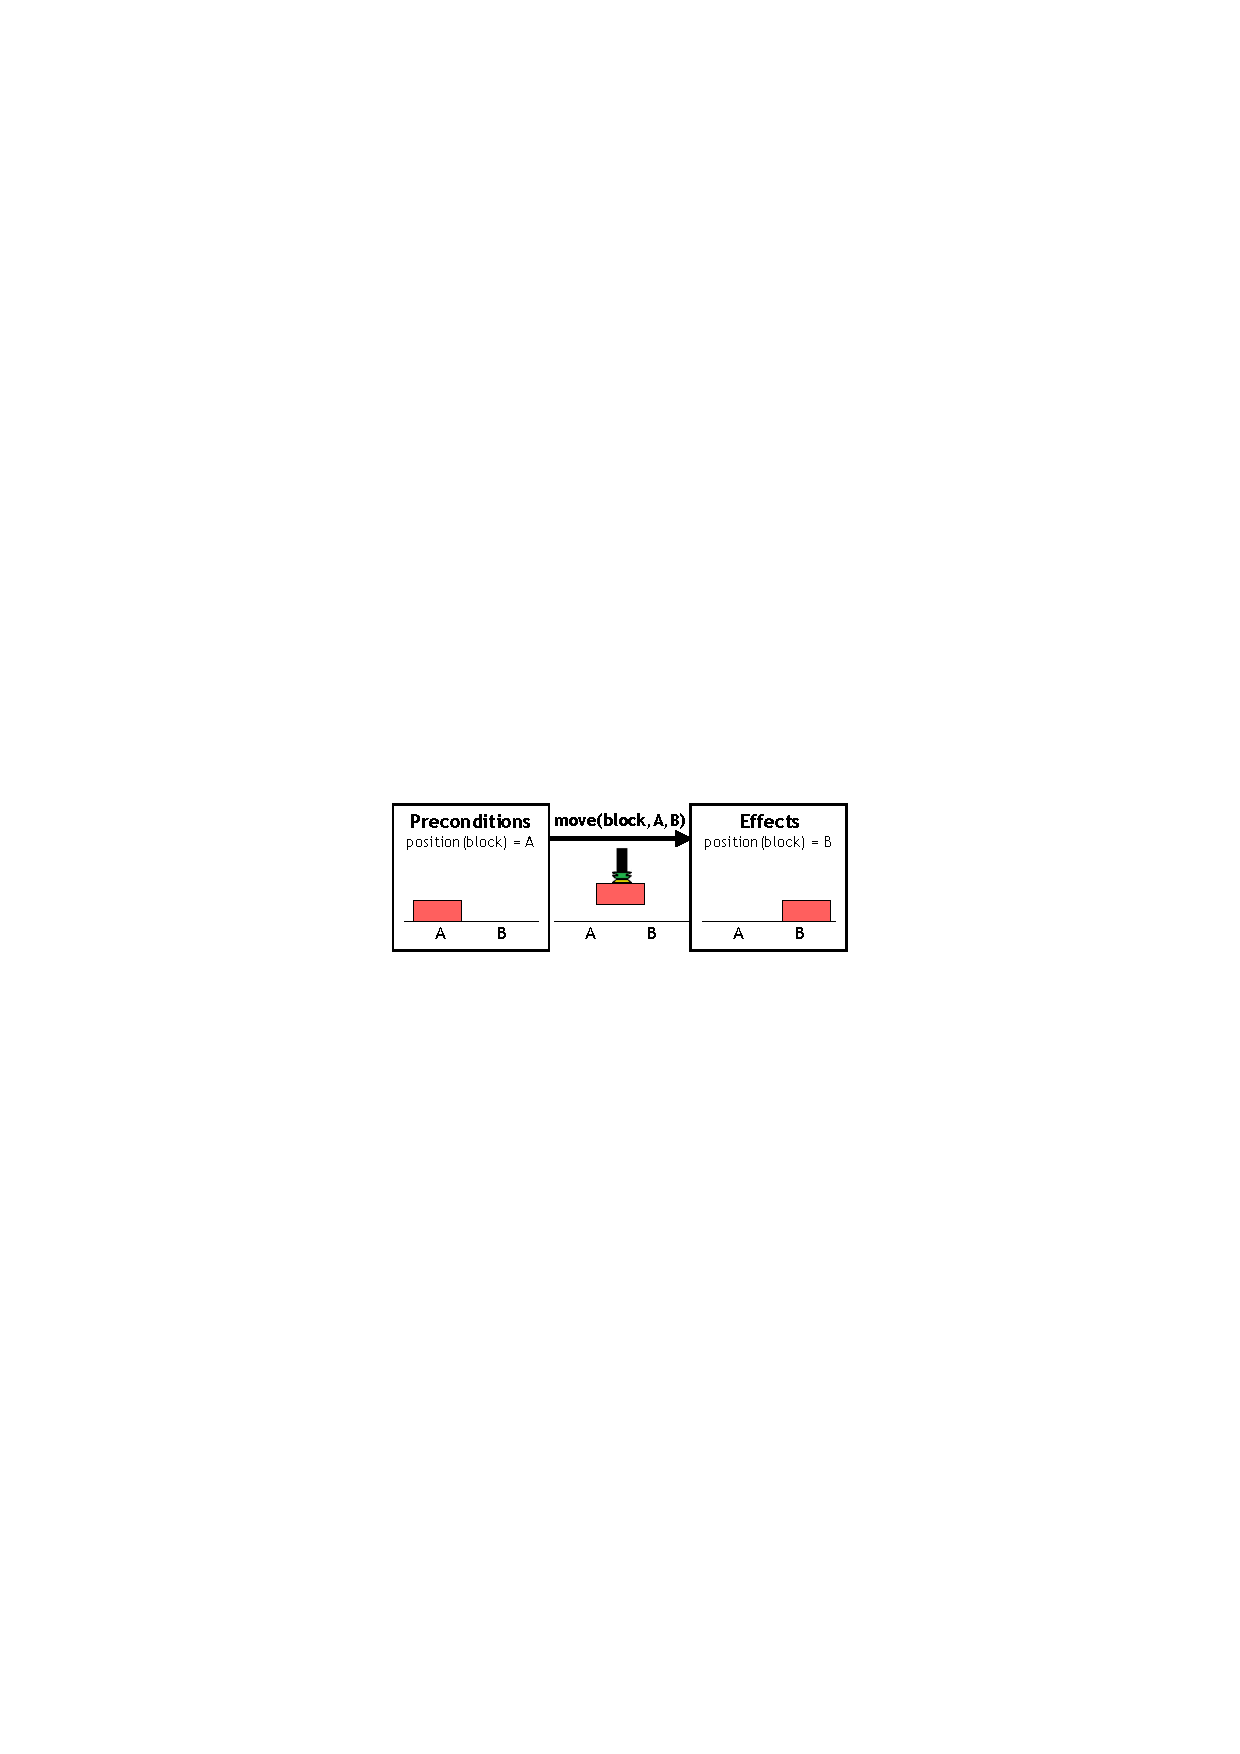
\includegraphics[width=.4\linewidth]{figures/schema-logic-1}
	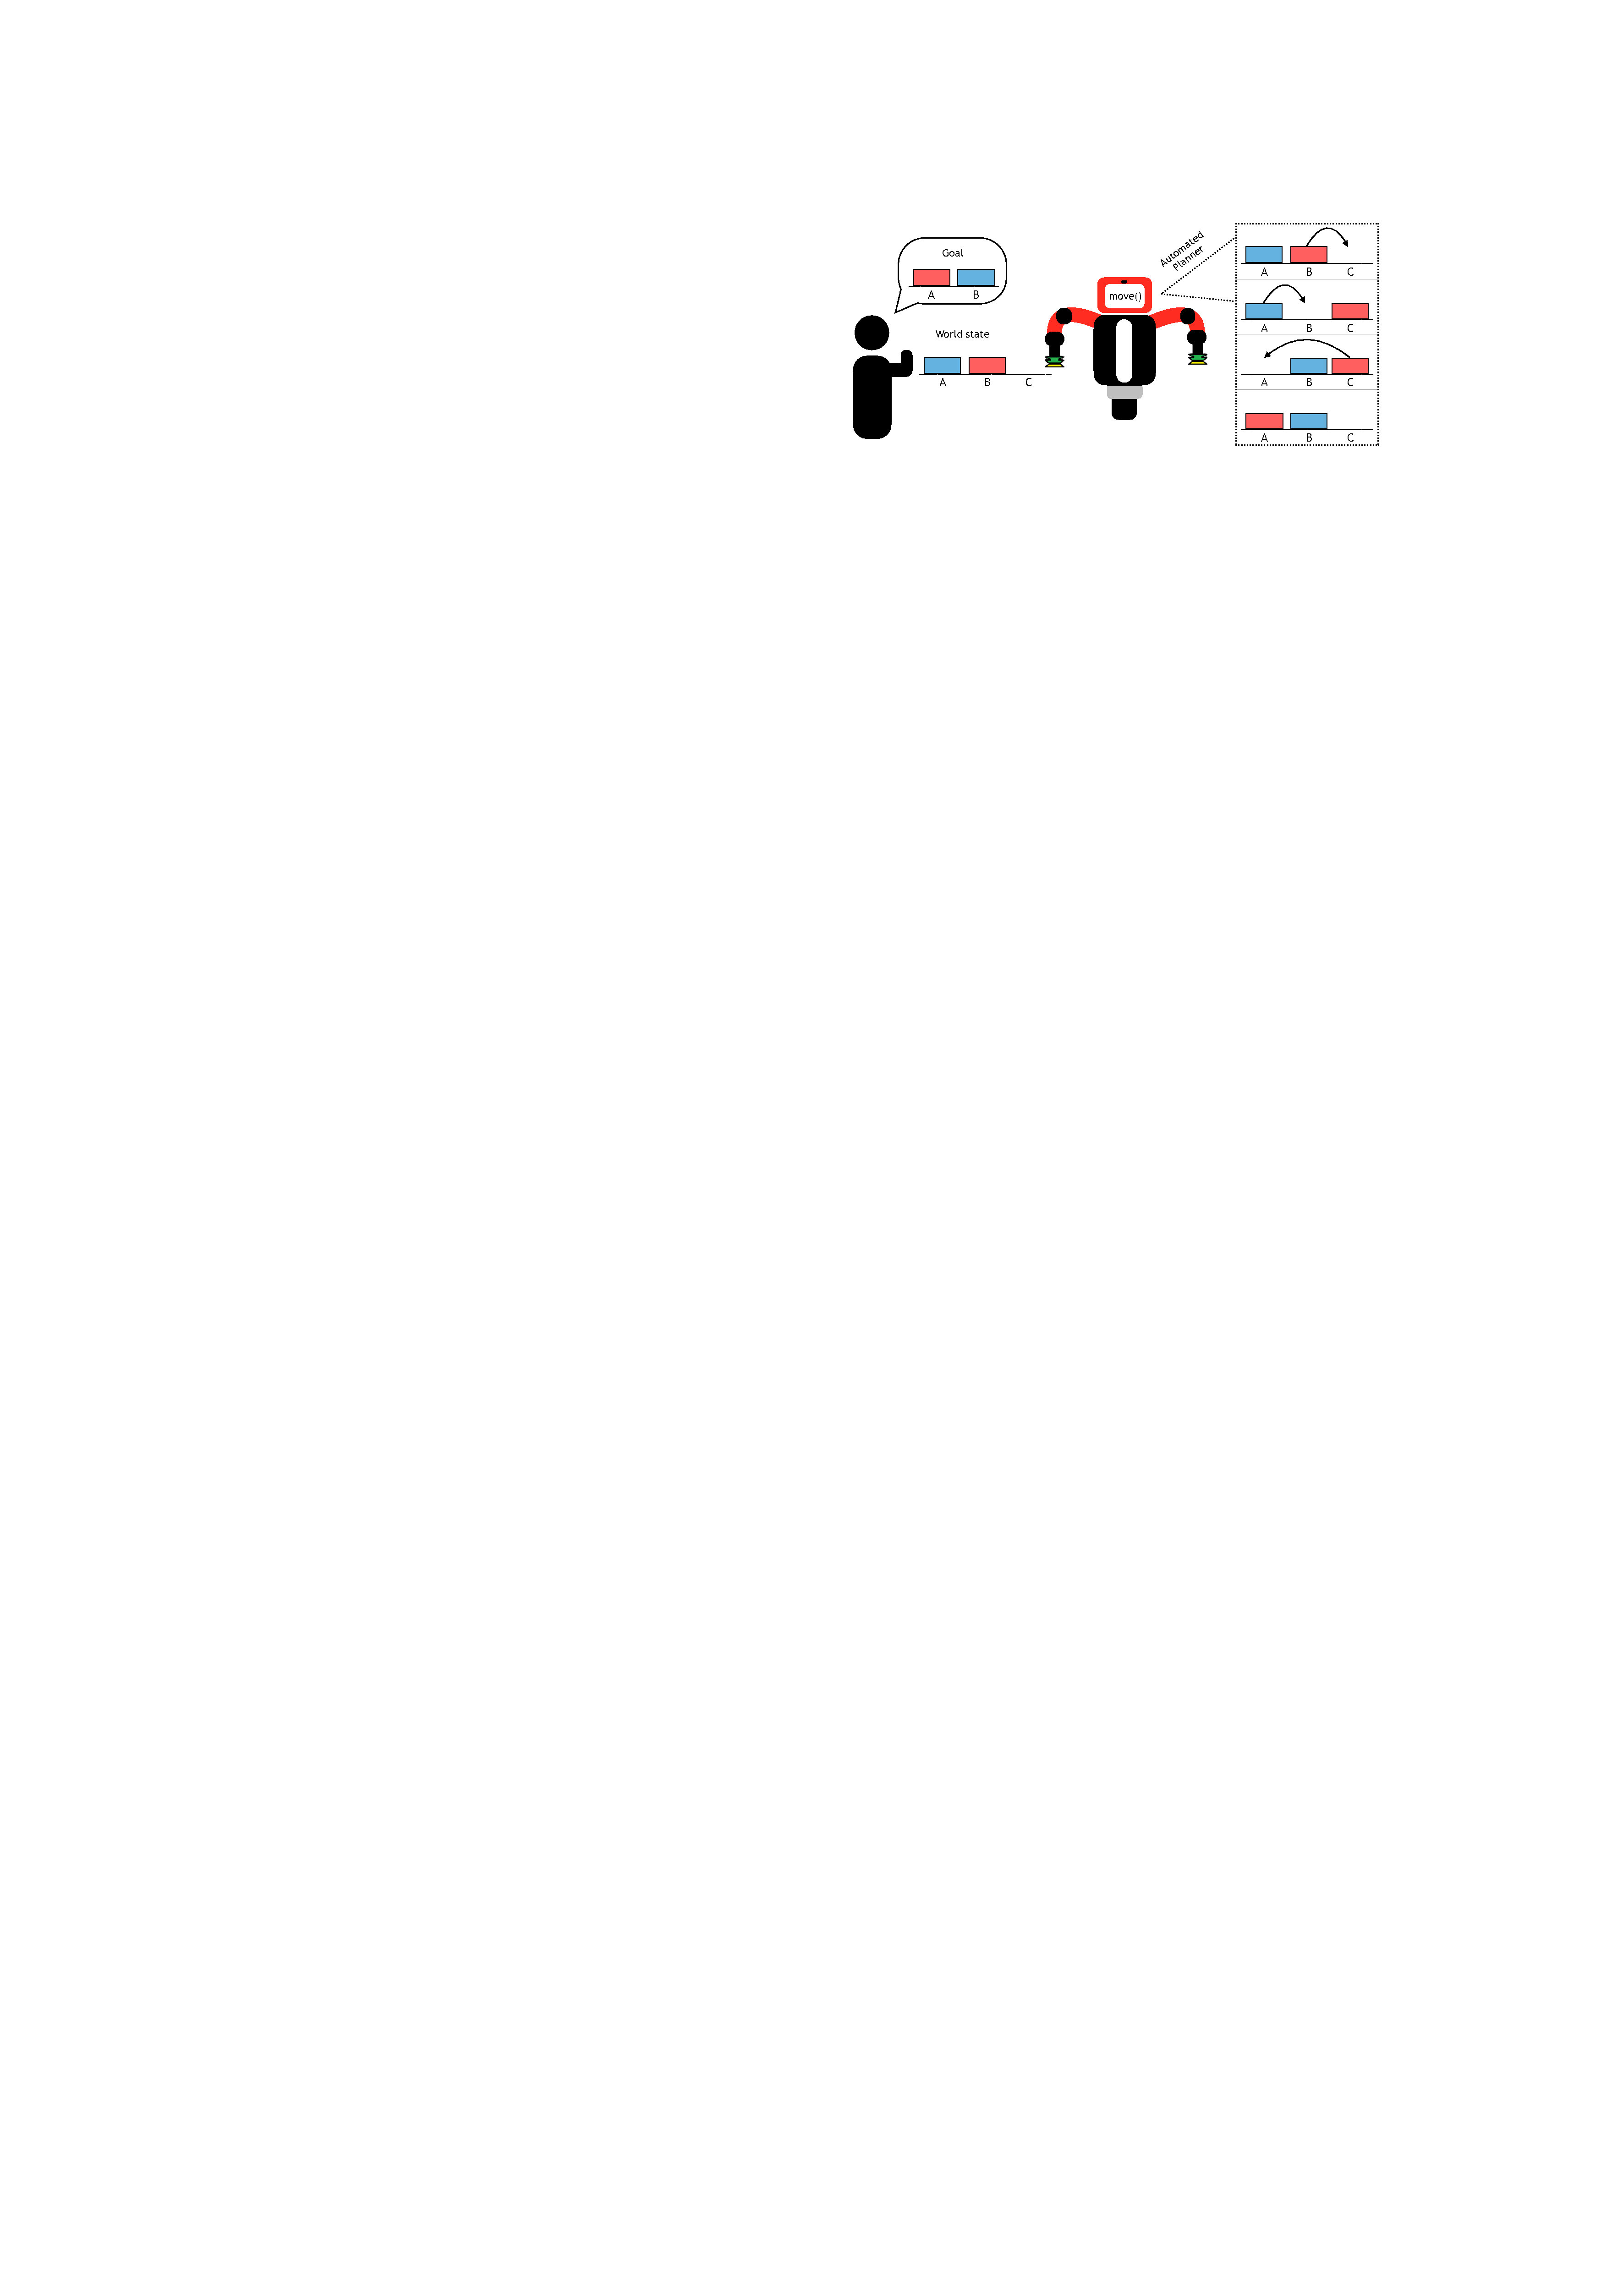
\includegraphics[width=.55\linewidth]{figures/PbD-AutomatedPlanner}
	\caption{Planning domain describing action model with preconditions and effects (left), an initial world state, goal state, and a generated action sequence (right).}
	\label{fig:Planning domain and action}
\end{figure}



\subsection{Problem Statement}
% limitations 
We need to consider the limitations: limited resources, lack of programming knowledge and time to train operators.
%, rather than atomic actions that can be reused independently 

We want the robot to generate solutions autonomously.
For this we need:
Automated planner - which as the robot's \textit{``brain"}
action models - actions with semantic meaning associated to it
PbD - end-user technique to teach robot an action

% semantics for application to new context
A robot that learns how to arrange items on a desk may have to plan the order of handling objects in another way than originally demonstrated by the teacher.
Thus, it does not suffice for the robot to replicate the demonstrated movement, but it needs to understand and interpret the teacher's intention so that it can apply the action to different scenarios.


In this thesis, we propose a framework that allows robots to solve problems in a goal-oriented way.
In other words, given a user-defined goal, the robot should generate and execute the right action sequence to obtain it.
The user must construct a knowledge base, consisting of a domain model (the environment that the robot interacts with) and all action models required for the robot to accomplish the defined task.

% example domain 
Consider again the Tower of Hanoi problem.
The domain model would consist of a table with a finite number of objects and limited positions, as well as actions consisting of pick, place and move. 
Possible goals could be to stack the objects by size (similar to the Tower of Hanoi problem) or to arrange the objects in a certain order. 
Our framework should enable the user to teach the robot by demonstration all action models needed, including their relevant preconditions and effects. 
Once the action models have been created, the inbuilt automated planner can generate an action sequence to achieve any goal within the domain. 

%Hence, we address two common situations, where reprogramming is required: 
%\begin{itemize}
%\item A new subtask needs to be included in the task execution, e.g. the robot knows how to place objects from any position on the table into a basket, but should additionally rotate them before placing them;
%\item All subtasks are available but the ultimate goal has changed, e.g. the order of placing the objects has been changed.
%\end{itemize}


\newpage
\section{Summary of contributions}
%\subsection{Thesis statement}
%Non-expert users can program a robot to complete a set of tasks by teaching it atomic actions by demonstration and correctly assigning them preconditions and effects that can be used with an automated planner to solve more complex problems.

In this thesis we propose a robot programming framework that allows human operators to:
\begin{itemize}
	\item teach the robot action models in a comprehensive automated planning representation, translated into PDDL, and
	\item enable it to use the learned action models to be controlled with a goal-oriented approach based on automated planning techniques.
\end{itemize}

With the focus on cobotic environments, we want to discover the difficulties encountered by the user, when faced with techniques in both Robot Programming by Demonstration and Automated Planning domains. 
The integration of a functioning real-world system would require solutions in perception (e.g. object identification), motion planning (e.g. manipulation, navigation, safety), human–robot interaction, and cognitive robotics (e.g. action learning, task planning). 
The integration of all aspects into a real-time system is a major challenge.
In this thesis we address this challenge and provide partial solutions for the other areas.
The contributions of this thesis can be summarised as follows:
\begin{itemize}
	\item {A robot programming framework that combines PbD and Automated Planning, where the robot learns action models by demonstration, and the problem of finding an action sequence is delegated to a planner.
	The robot programming process consists of steps:
	\begin{enumerate}
		\item the non-expert user demonstrates atomic actions to the robot, and teaches \textit{action models}, expressed in a symbolic planning language (STRIPS \cite{fikes1971strips}),
		\item the robot uses these action models with an automated planner to generate solutions to user-defined goals,
		\item the user can revisit the taught action model to refine them.
	\end{enumerate}}
    \item {Experimental findings on user acceptance of the proposed robot programming framework, when users are tasked to teach a robot by demonstration and correctly assign action conditions used for automated planning. \\
    Research question: \textit{Can users teach a robot action models for automated planning using the robot programming framework?}}
    \item {Experimental findings on issues encountered when non-experts are tasked to use AI planning and PDDL concepts to describe a domain model to a robot. 
    	We evaluated the user's ability to construct symbolic action models, in terms of preconditions and effects, used by automated planners.\\ 
    Research question: \textit{How do non-expert users adopt the automated planning language with its action model representation?}}
    \item {System for robotic shelf organisation tasks: simultaneous end-user programming of goals and actions using PbD and interactive visualisation. \todo{elaborate}}
\end{itemize}


\section{Document organization}
This thesis is organised as follows. 

\paragraph{\chapt{chap:Sota}} gives an overview of the state of the art in Robot Programming.

\paragraph{\chapt{chap:Sota-PbD} and \chapt{chap:Sota-AP}} cover definitions and state of the art of Programming by Demonstration and Automated Planning respectively.

\paragraph{\chapt{chap:Contribution}} presents our proposed solution as as Robot Programming Framework for End-Users.

%\paragraph{\chapt{chap:Implementation}} details our achieved implementation of the framework. 

\paragraph{\chapt{chap:Evaluation}} presents preliminary results in terms of qualitative experiments for evaluating our framework. We present experimental findings on user acceptance and issues encountered when introduced to the AI planning concepts.

\paragraph{\chapt{chap:OrganisingTasks}} presents the work on shelf organising tasks for simultaneous end-user programming of goals and actions.

\paragraph{\chapt{chap:Conclusion}} concludes our work and discusses possibilities for future implementations of the framework.

\part{Literature Review}\label{part1}
 \cleardoublepage
\chapter{Robot Programming}\label{chap:Sota}
\minitoc% Creating an actual minitoc

%In this section we give an overview of common robot programming techniques.
%We present different approaches for both manual and automatic programming systems and situate our thesis in relation to these approaches.

In this thesis, we consider the definition of robot programming to be the following: 

\theoremstyle{definition}
\begin{definition}{Robot Programming}
is the process of defining desired motions and associated skills so that the robot may perform them without human intervention.
\end{definition}

There are many ways to divide robot programming systems. \cite{lozano1983robot} divided them into three categories: guiding systems, robot-level programming systems, and task-level programming systems. However, the range of programming systems was very limited at that time and examined only industrial robot programming systems.
\cite{Biggs2003} took a different approach and divided them into two categories to distinguish systems for users and for programmers:

\begin{itemize}
  \item Manual programming, where the user can directly control the robot's execution code 
  \item Automatic programming, where the user does not need to write explicit code
\end{itemize}
% - also mention software architectures which are important for any robot programming systems.

 \begin{figure}[ht]
 \centering
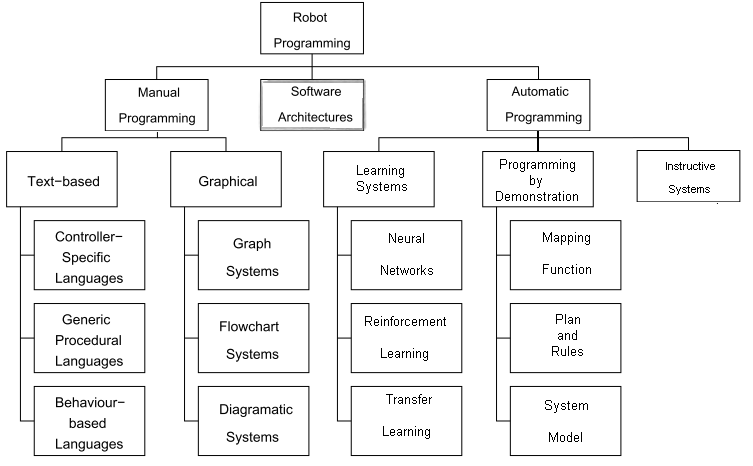
\includegraphics[width=\linewidth]{figures/Biggs2003-RobotProgramming}
 \caption{Robot programming categories to distinguish systems for users and programmers. \cite{Biggs2003}}
 \label{fig:RobotProgrammingSystems}
\end{figure} 

In the following sections we will give a brief overview of the different programming systems.

\begin{table}[ht]
\begin{center}
\begin{tabular}{r|c|c}
Programming Techniques & by Exploration \newline (unguided) & by Demonstration \newline (guided)\\ \hline
Classification & \checkmark & \checkmark \cite{saunders2006teaching,hovland1996skill,rybski1999interactive} \\
Regression & \checkmark & \checkmark \cite{atkeson1997locally,pomerleau1991efficient} \\
Reinforcement Learning & \checkmark & \checkmark (System models) \cite{atkeson1997robot,smart2002effective,abbeel2004apprenticeship}.\\
 Plans & \checkmark & \checkmark \cite{kuniyoshi1994learning,ekvall2008robot} \\
 \hline
Human-Robot Interaction & & \\ \hline
 touch & \checkmark (learning by poking) & \checkmark \\
 vision & \checkmark & \checkmark \\ 
 voice & n/a & \checkmark (instructive, create sequence by voice) \\
\end{tabular}
\end{center}
\label{tab:Programming Overview}
\end{table}



 \begin{figure}[ht]
 \centering
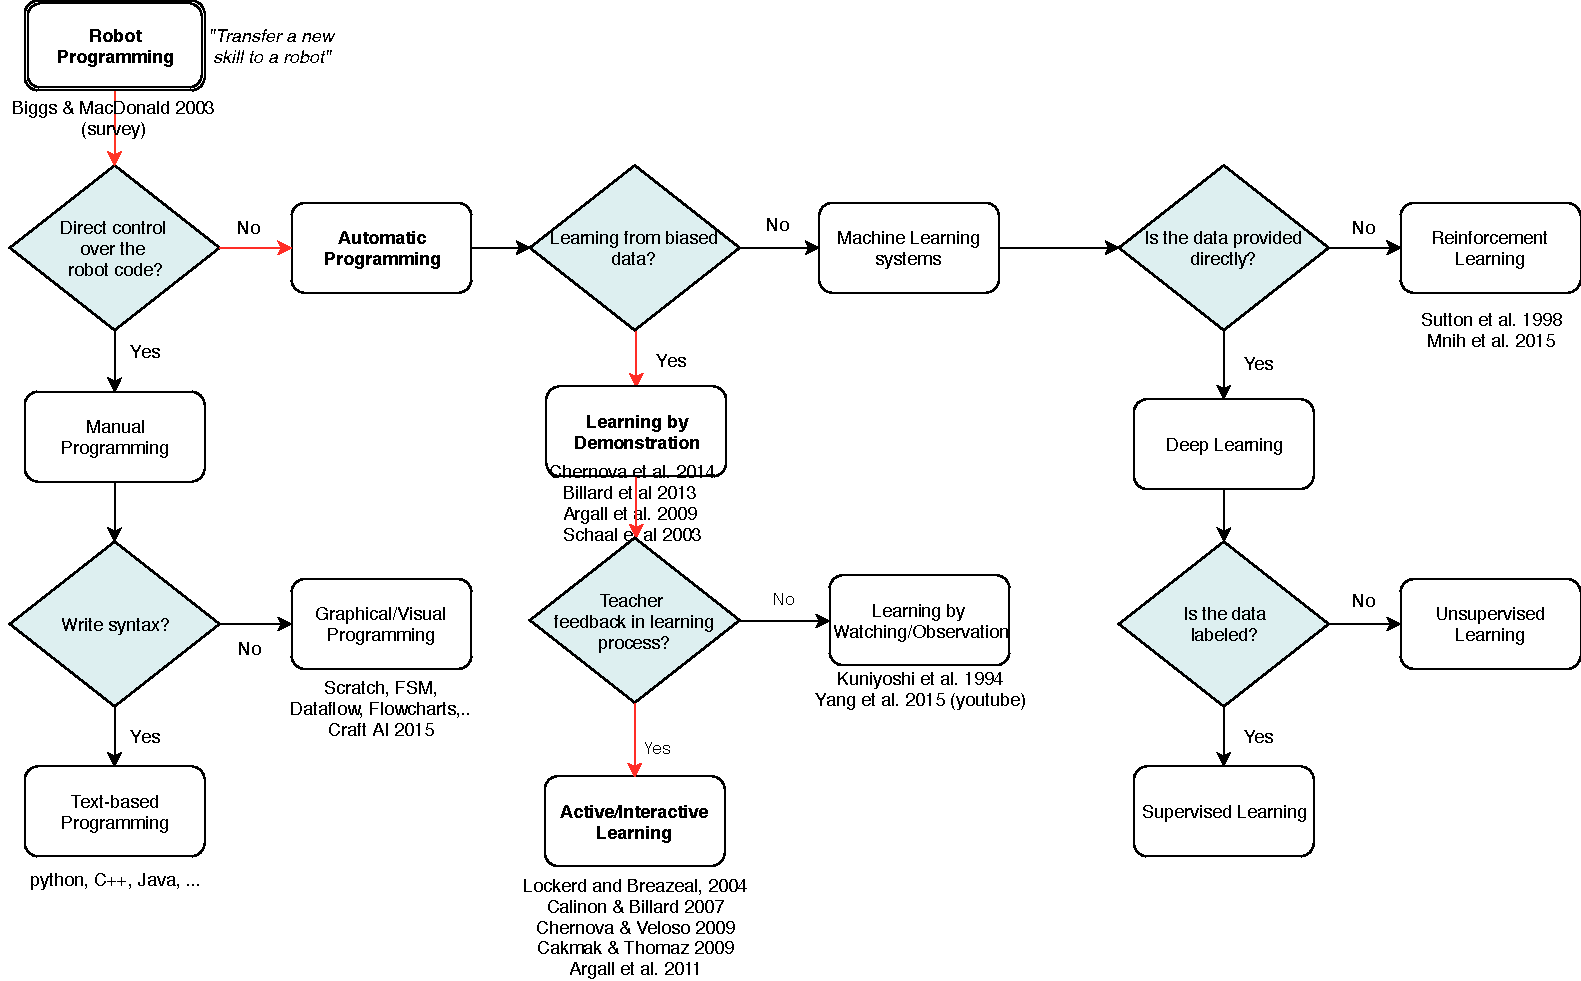
\includegraphics[width=\linewidth]{figures/RobotProgrammingOverview.pdf}
 \caption{Overview of Robot Programming methods.}
 \label{fig:RobotProgrammingOverview}
\end{figure} 

\subsection{Manual Programming Systems}\label{subsec:Manual Programming Systems}
In manual programming systems users must create the robot program by hand, either using a text-based or a graphical interface.
While the user has direct control over the robot code, it requires expert knowledge in a programming language, which is often a rare resource in industrial environments.
There exist a variety of tools to make programming, as well as testing and debugging easier, such as IDEs, spreadsheets, macros.
There are two types of manual programming: text-based programming, where the code is written manually in a chosen programming language (python, C++, java, etc.) and graphical programming, where the code structure is created with the help of a graphical interface (e.g. Scratch (Majed 2014, Lamb \& Johnson 2011, Schorow 2007), Flowcharts,..). 

\paragraph{Classical robot programming}\label{par:Classical RP}
Classical robot programming processes in the industry have task-specific definitions, which are generally robot-dependent, and require programming expertise.
\fig{fig:Classical robot programming process} shows the classical robot programming process.
After the initial task definition, an optimal sequence of the workcell operations is defined.
Once the process has been validated, the robot is programmed offline in its native language, before it is pushed into production for regular execution.
The programmed robot can only be used for this specific task, in this particular working environment.
If the task definition needs to be altered, the programming expert needs to repeat the entire programming process.
Therefore, classical robot programming processes are time consuming and cost intensive.

\subsubsection{Text-based Systems}\label{sssec:Text-based Systems}
Text-based systems are one of the most common methods and use a traditional programming language approach. 
Depending on the type of language used, the user performs programming in controller-specific, generic procedural or behaviour-based languages.
Despite the trend to move from simple, command-based languages towards more intelligent programming systems with high-level languages that provide more support to the user, text-based systems still require trained users with programming knowledge and are more likely to be used by robot developers than end-users.

\subsubsection{Graphical Systems}\label{sssec:Graphical systems}
Graphical (or icon-based) systems use a graph, flow-chart or diagram view where users manually specify actions and program flow. They are typically easy to use and generally used for robot applications rather than system programming. \cite{lego2003} and \cite{bischoff2002morpha} produced graphical systems using a flow-chart approach, where the robot's behaviour can be configured by arranging low-level actions in a sequence.
\todo{Add examples of graphical systems}

\begin{figure}[ht]
	\centering
	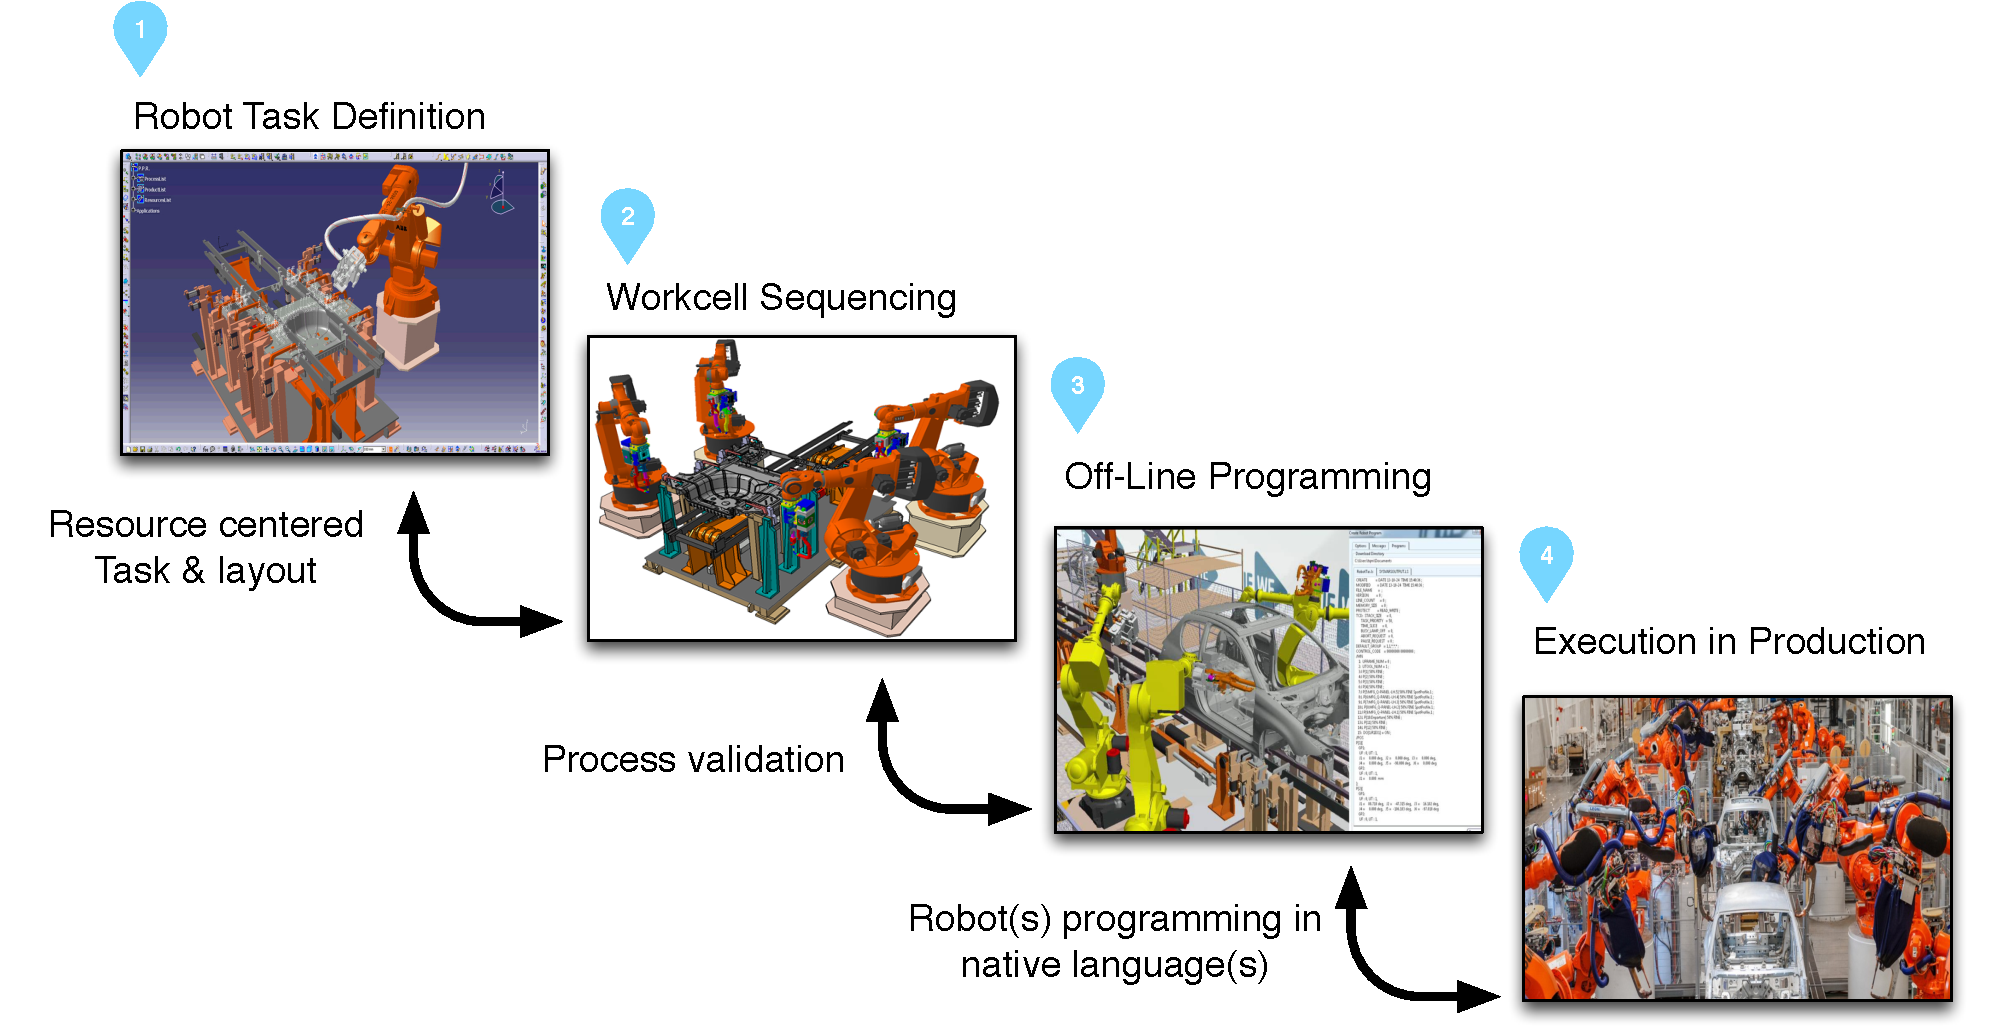
\includegraphics[width=\linewidth]{figures/manual-programming}
	\caption{Classical robot programming process}
	\label{fig:Classical robot programming process}
\end{figure}


\subsection{Automatic Programming Systems}\label{subsec:Automatic Programming Systems}
Automatic programming relates to robots that have the capability to learn from new data.
Unlike manual programming, the user does not need to write explicit robot code and does not have direct control over the code as its behaviour is generated from information entered into the system.
We distinguish between systems that are \textit{guided}, where the robot learns with human intervention (e.g. Programming by Demonstration), and \textit{unguided}, where the robot learns by exploration (e.g. Neural Networks, Reinforcement Learning).
Inspired by \cite{Biggs2003}, we further divide automatic systems into two categories: learning systems (unguided) and programming by demonstration (guided).

\subsubsection{Learning Systems}\label{sssec:Learning Systems}
Learning systems use inductive inference to create a program by taking examples provided by the user or from self-exploration of the robot. The goal of so-called machine learning (ML) systems is to construct programs that allow the robot to automatically improve its performance with increasing data. Even though machine learning algorithms have been around since the 1980s \cite{}, it has only become popular in the past few decades. The rise of the internet led to big data and developments in various research areas such as machine learning and computer vision, which have impacted the field of robotics.
The increasing amount of big data and advances in techniques to process and store data efficiently has lead to a wave of new machine learning techniques. 

\cite{Kreuziger1992} analysed the application of ML in robotics (\fig{fig:MLvsRobotics}) and identified a large gap between these two research areas.


 \begin{figure}[ht]
 \centering
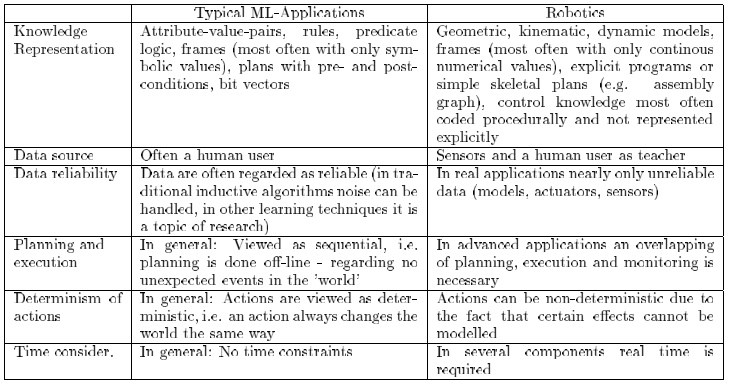
\includegraphics[width=\linewidth]{figures/Kreuziger1992-Comparison ML Robotics}
 \caption{Comparison on Machine Learning applications vs. Robotics. \cite{Kreuziger1992}}
 \label{fig:MLvsRobotics}
\end{figure} 

\cite{kaiser1995obtaining} 

Recently Machine learning techniques have found their application in robotics. Research areas include: \url{http://techemergence.com/machine-learning-in-robotics/}\\
computer vision (or ``robot vision'') for the identification and sorting of objects \cite{stager2013computer} or to learn action plans from watching unconstrained videos \cite{Yang2015}.

These systems can use neural networks (NN) \cite{billard2001robust} or reinforcement learning (RL) \cite{smart2002effective}. Both NN and RL require a large amount of data to learn the desired behaviour. 
RL further requires a reward function which needs to be specified by a domain expert.
There are two main classes of RL approaches, namely model-based \cite{polydoros2017survey} and model-free \cite{kober2013reinforcement} methods, differentiating between whether a model of the interactions between the robot and the environment is used, or whether it learns from samples.
While model-based methods converge faster to the optimal solution, an accurate model is not always available and can impact the learning process.
Model-free methods require the robot to learn from samples, resulting in a slow convergence to the optimal solution.
To accelerate the learning and reduce the amount of exploration required, work has been done to include teacher demonstrations with RL solutions \cite{martinez2017relational,hester2017learning}.
In real world scenarios robots require teacher input to learn behaviours efficiently. 
\todo{Similar to our work: \cite{martinez2017relational}}

The problem with RL solutions is that reward functions are difficult to specify.
Inverse reinforcement learning \cite{abbeel2011inverse} is a supervised RL mode where the learner tries to acquire the reward function from demonstrated behaviours.
This is can also be considered a learning from demonstration approach.

\subsubsection{Programming by Demonstration}
Programming by demonstration (PbD) \cite{billard2008robot}, also known as Learning from Demonstration, describes various techniques the robot learns new behaviours from teacher demonstrations. 
There are different ways for a teacher to provide demonstration data (\sect{subsec:Gathering demonstrations}), depending on the amount of data provided at a time (incremental vs. batch learning) and the different interaction modalities (touch, vision, gestures, voice) to transfer the data to the robot. 
The robot derives a policy in various ways (\sect{subsec:Deriving a policy}). 

PbD systems have been used in the industry for creating assembly programs. 
In recent years there has been significant work in PbD to move from pure imitation to intelligent systems that learn flexible task executions. 
PbD systems may learn task descriptions from interpreted data to adapt the learned task to changing environments.

\subsubsection{Instructive Systems}\todo{Delete or Move}
Instructive systems use gesture or voice recognition to command robots to carry out tasks.
These tasks typically consist of actions that they have already been trained or programmed to do. 
Gestures can be used to direct the attention of the robot for indicating objects in a scene to which the instructions apply. 
Natural language is the most intuitive way for humans to communicate instructions but may need some form of clarification and learning system in order to work efficiently. 
A multi-modal communication including information from vision, gesture and voice sources can be used to clarify instructions to the robot, for example mentioning ``that table" and gesturing the relevant object.
Instructive systems are useful for providing a high-level control but rely on underlying trained abilities which need to be implemented using other programming systems such as manual programming or PbD.

\subsection{Robot Programming in Industrial Environments}\label{subsec:RP in Industrial Enviroments}
\cite{pan2012recent} gives an overview of three main robot programming methods for industrial robots: online programming, offline programming (OLP), and robot programming using Augmented Reality (RPAR). 

\subsubsection{Online Programming}\label{sssec:Online Programming}
In online programming methods the robot program commands the robot to move through a recorded sequence of end-effector postures which form a complete task. 
The postures are recorded using the teach pendant to manually move the end-effector to the desired position and orientation of the task. 
Due to its simplicity, intuitiveness, and low programming skill requirement, this method is widely used. 
However, it is only suitable for programming applications with uncomplicated processes and work pieces with simple geometry. 
Once the program has been generated, it is difficult to make further amendments.

\subsubsection{Offline Programming}\label{sssec:Offline Programming}
Offline Programming (OLP) is based on 3D CAD data that models the complete robot work cell and lets the user fine-tune the properties of the robot's movements before generating a program that can be downloaded to the robot. 
It is more efficient when programming complex systems with large volumes and more reliable compared to online programming. 
As it requires a great amount of programming effort and a long delivery time, it requires high programming overhead and is not efficient for the development of smaller product volumes or customised software.

Robot designers and users have developed computational platforms for OLP systems in form of packages that allow secondary development for specific applications. 
These OLP packages simulate not only robot trajectories and assembly tasks, but can also model interactions of several manufacturing processes, resources and product maintenance issues. 
Almost every robot manufacturer has its own OLP software. 
There exist also generic OLP software that are more flexible for hardware from different manufacturers.

Current OLP systems do not provide functions for the complete OLP process but include steps that need to be created manually. 
Due to the high costs of OLP systems, their use is not cost-efficient for small to medium-sized enterprises.

\subsubsection{Augmented Reality}\label{sssec:Augmented Reality}
The use of augmented reality (AR) is a revolutionary concept where computer-generated 3D objects are blended onto a real world scene to enhance the user's interaction with the real world \cite{pettersen2003augmented}. 
Robot programming using AR allows offline programming to be performed without the need to model the workpiece in the virtual environment \cite{pan2012recent}. 
It can eliminate technical difficulties faced by OLP techniques such as the calibration between the virtual and the real world.

We aim to provide a solution for non-expert users to program robots in the industry without writing code. 
We want to learn a high-level abstraction of the behaviours that can be combined with the PDDL language.
%\section{End-user Development}
\subsection{What is EUD?}
- End-User Development can be defined as a set of methods, techniques, and tools that allow users of software systems, who are acting as non-professional software developers, at some point to create, modify or extend a software artefact. \\
- main goal of EUD: empowering end-users to develop and adapt systems themselves\\
- must be made considerably more flexible and they must support the demanding task of EUD: they must be easy to understand, to learn, to use, and to teach\\
- easy to test and assess their EUD activities\\
 (\cite{lieberman2006end})
 
\subsection{Types of EUD}
1. Parameterisation or Customisation 

2. Program Creation and Modification : Programming by Example, Incremental Programming, Model-based development, Extended annotation or parameterisation .\\
 
\subsection{EUD interaction styles} 

Programming is.....\\
- using visual attributes\\
- by demonstration\\
- by specification\\
- with text\\
 (Scaffidi2011enduser)\\
 
 \subsection{Design guidelines for EUD systems}
  (\cite{ko2004six}), (\cite{repenning2006makes})
 
\subsection{Definitions}
- Programming\\
- Interactive vs Batch\\
- Visual programming (VP): graphics are the program itself, e.g. flow charts and graphical programming languages, Scratch, \\
- Program visualization (PV): program is specified in textual manner and graphics illustrate some aspect of the program, \\
- Programming by Example\\
 (Myers1986visual) defines VP vs PbE vs batch/interactive
 
\subsection{Challenges of EUD}
- limited human patience and inconsistent user input
 
 
\subsection{Design choices to implement interactive machine learning methods}
(\cite{chernova2014robot})
Where to have teacher's input? Where to have robot influence/decide?\\
- Data collection: what training data to include? \\
- Selecting the feature space and its structure: include input features that are in fact discriminatory \\
- Defining a reward function that represents the task learned \\
- Subtasking the problem: determine the task structure \\



\section{Discussions and Relations to Present Work}
The problem with manual programming systems is the need for programming expertise and high programming time and effort required to debug and test.
The solutions are often task-specific and cannot be changed easily by end-users.

Automatic programming systems require significantly less effort when it comes to the programming process. 
However, machine learning systems using Neural Networks often need large amounts of training data and data that is relevant for the desired application scenario.
Reinforcement Learning solutions can be time-consuming as they require the robot to explore the environment and collect the necessary data to learn the optimal policy.
There is on-going research to reduce the amount of data and time required to learn the optimal policy.
When deploying robots in real world applications, both manual and machine learning systems become cost-expensive and inefficient to adapt to different tasks.
A feasible automatic programming system can involve a human operator teach the robot the desired tasks.


\subsection{Relation to Present Work}
In this thesis we choose Programming by Demonstration as the robot programming solution for end-users, as it is an intuitive technique for teaching the robot new tasks with minimal programming overhead.
There exist a wide range of robot grippers (claw, suction, magnetic, etc.) that are dependent on the robot.
With PbD the robot can be taught a user-specific task, independent of the robot's architecture.
Robots are currently being used for many industrial applications from welding (arc welding, spot welding, etc.) to material handling (pick and place, packaging, palletizing, etc.).
In this work we focus on teaching robots material handling tasks, in particular pick and place tasks.
The problem we address is two-fold:
\paragraph{Teaching atomic actions.}
Existing PbD implementations are rather task-specific and cannot be applied to arbitrary scenarios.
Many PbD implementations already have pick and place actions coded into the system (\cite{veeraraghavan2008teaching}) and the robot is taught an action sequence to achieve a predefined goal.
Even slight changes in the goal could require a different action sequence, so the robot needs to be taught the new action sequence.
This highlights a key issue in PbD, namely, to design a system that allows the robot to learn  generic tasks that are applicable to different scenarios.
In this work, we assume that the robot does not have any atomic actions preprogrammed.
The user should be able to teach the robot atomic actions by demonstration, which are can be used to generate the action sequence.

\paragraph{Automatic action sequence generation.}
After having learned all atomic actions, the robot needs to reuse these actions to achieve a goal.
Current solutions either teach the robot entire action sequences or include an intermediate manual step where the user has to construct an optimal sequences.
Finding an optimal sequence can be tedious and expensive.
%We want to equip the robot with all the skills needed to act autonomously in any state of the world, rather than teaching it how to react to a given state of the world.
%To achieve this, we have to design our framework using plans, which provides us with the required tools.
%As we focus on collaborative environments, where the teacher is actively involved in the learning process, plans allow a means to communicate the teacher's intentions together with the demonstrations.
Thus, we use Automated Planning techniques, to generate action sequences automatically.
%This will enable the robot to learn the action and its semantics, so that an action sequence can be generated automatically with the help of a planner. 

\paragraph{}
In the following sections we will discuss both Programming by demonstration and Automated planning in further detail.


\cleardoublepage
\chapter{Automated Planning}\label{chap:Sota-AP}
\minitoc% Creating an actual minitoc
In this section we give a brief overview on Automated Planning.
We present the theoretical definitions and representations (\sect{subsec:Classical planning problem}), the standard encoding language PDDL (\sect{subsec:PDDL}), and discuss knowledge engineering tools for creating planning domains (\sect{subsec:Knowledge Engineering}).
%, and situate our thesis in relation to these approaches.

%%%%%%%%%%% ******  AUTOMATED PLANNING ******* %%%%%%%%%%%%%
\section{Introduction}
\begin{center}
\textit{``Planning is an important component of rational behaviour." }\\ \cite{ghallab2004automated}
\end{center}

% \begin{center}
% \textit{``A goal without a plan is just a wish."}\\
% - Antoine de Saint-Exup\'{e}ry
% \end{center}

% Introduction/Definition
Automated planning, also known as AI planning, is an area in A.I. that studies the deliberation process of choosing and organising actions to achieve a goal. 
Humans automatically anticipate the outcome of their actions, even if they are not fully aware of it. 
Automated planning techniques are used to create information processing tools that efficiently reproduce human reasoning and behaviour. 
In particular, it can be used to model a robot's skills and strategies, when operating in diverse environments, without the need for expensive hand-coding.

The focus in automated planning lies within the development of {domain-independent} planning systems, called \textit{planners}.
These planners consist of search algorithms, which are not problem-specific, hence generate solutions to problems, no matter what the input. 
Given a set of actions, a description of the state of the world, and some goal state, the planner generates an ordered sequence of actions, which guarantees the transition from the initial state to the goal state. 
Similar to the policy derivation method mentioned in \sect{subsec:Deriving a policy}, actions are defined with \textit{preconditions}, i.e. conditions on the state of the world in order to execute the action, and \textit{effects}, i.e. changes in the state of the world after the action execution. 
%The planner produces an ordered sequence of actions, known as a \textit{plan}, which guarantees the transition from the initial state to the goal state.

% Example
An example of a planning problem is the Tower of Hanoi problem (\cite{douglas1985metamagical}), where the world objects are three pegs and disks of different sizes. 
In the initial state, the disks are stacked in ascending order (smallest at the top) on one of the pegs, in the goal state the disks are stacked in the same order on one of the other two remaining pegs. 
The goal state must be achieved by obeying certain rules for moving the disks (e.g. only the top disk of a stack can be moved at a time and may not be placed on top of a smaller disk). 

There exist different types of planning (\cite{ROSplanAAAI17tutorial}):
\begin{itemize}
    \item Classical planning
    \item Optimisation: minimise or maximise a given cost function
    \item Temporal planning: actions have a certain duration, to address concurrency, synchronisation, time dependent effects.
    \item Planning with preferences: prefer hard goals over soft goals.
    \item Conditional planning: actions can perform observations, plan contains branches
\end{itemize}

\subsection{Classical planning problem}\label{subsec:Classical planning problem}
In classical planning, world dynamics are modelled as state transition systems.

\paragraph{Definition.}
A \textit{state transition system} is a triple $\Sigma = (S, A, \gamma)$ such that:
\begin{itemize}
\item $S$ is a finite set of states,
\item $A$ is a set of actions,
%\item $c : A \rightarrow \mathbb{R}^{+}$ is a cost function,
\item $\gamma : S \times A \rightarrow S$ is a state transition function.
\end{itemize}

\noindent A state transition system can be represented as a directed graph whose nodes are states of $S$, and arcs are actions of $A$. 
Applying an action $a$ to a state $s$ produces a new state $s'= \gamma(s,a)$ 
%with a cost $c(a)$
. 
$\Sigma$ is deterministic if for all states $s$ and actions $a$, the transition function $\gamma(a, s)$ produces a unique state $s'$. 
%$\Sigma$ has a unit cost if, for all $a \in A$, $c(a) = 1$. 
A \textit{plan} is any sequence of $k$ actions $\pi = <a_1,\cdots, a_k>$. The state produced by applying $\pi$ to a state $s$ is the state obtained by applying each action of $\pi$ sequentially. 
We can denote this by extending the state transition function to plans as follows:
\[\gamma(s,\pi)=\left\{
\begin{array}{ll}
   s, &\mbox{if $k=0$} \\
   \gamma(\gamma(s,a_1),<a_2,\cdots, a_k>), &\mbox{if $k>0$ and $a_1$ is applicable to $s$} \\
   \mbox{undefined}, &\mbox{otherwise}
\end{array}
\right.
\]
A state $s_n$ is reachable from a state $s_0$, if there exists a plan $\pi$ such that $s_{n} = \gamma(s_0, \pi)$.\\

%\subsubsection{Classical Planning Representations}

%Classical planning problems can be represented in three different ways, each of them being equivalent in expressive power: \cite{ghallab2004automated}

%\begin{itemize}
%\item Set-theoretic representation: each state of the world is a set of propositions, each action is a syntactic expression specifying which propositions belong to the state in order for the action to be applicable (e.g. \texttt{ontable-red, ontable-blue, on-red-blue, holding-red, holding-blue, stack-red-blue})
%\item Classical representation: states and actions are like the ones in set-theoretic representations except that first-order literals and logical connectives are used instead of propositions (e.g. \texttt{ontable(x), on(x,y), holding(x), stack(x,y)} )
%\item State-variable representation: each state is represented by a tuple of values of n state variables \{\texttt{red, blue,\dots, table, 1, 0, nil}\} (e.g. \texttt{pos(x) = table, pos(x) = y, holding = x, stack(x: block, y: block)})
%\end{itemize}

%\noindent The set-theoretic representation can take up much more space than the classical representation. The state-variable representation is less natural for logicians but useful for non-classical planning problems to handle numbers, function and time. The classical representation is the most popular choice for restricted state-transition systems \cite{ghallab2004automated}.

\noindent Logical representations are one of the most commonly used representations for classical planning problems. Each state of the world $s$ is represented by a set of logical propositions $p_i$, denoting facts of the world that are \textit{true} in the state $s$. If $p$ is not in the state $s$, it is considered to be \textit{false}.
\textit{Planning operators} change the state of the world by modifying the truth values of the propositions. An operator is defined by a set of propositions, which have to be true in a state in order to apply the changes (\textit{preconditions}), and a set of propositions, which will be true or false after the application of the action (\textit{effects}).

\paragraph{Definition.}
\noindent A \textit{planning operator} $o$ is a tuple $o = (\text{name}(o), \text{precond}(o),$ $\text{effect}(o))$, whose elements are as follows:
\begin{itemize}
\item $\text{name}(o)$ is the {\em name} of the operator,
\item $\text{precond}(o)$ is a set of literals that must be true to apply the operator $o$,
\item $\text{effect}(o)^{-}$ is a set of literals that are false after the application of the operator $o$,
\item $\text{effect}(o)^{+}$ is a set of literals that are true after the application of the operator $o$.
\end{itemize}

\paragraph{Definition.}
\noindent An \textit{action} is any ground instance of an operator. If $a$ is an action and $s$ is a state such that $\text{precond}(a)$ are true in $s$, then $a$ is {\em applicable} to $s$ and the result of applying action $a$ to state $s$ is the state $s'$:  
\[s' = \gamma(s, a) = (s - \text{effects}^{-}(a)) \cup \text{effects}^{+}(a).\]

\paragraph{Definition.}
A \textit{planning problem} in the logical representation is a quadruplet $(P, A, I, G)$ where:
\begin{itemize}
\item $P$ is a finite set of propositions,
\item $A$ is a finite set of actions,
%\item $c : A \rightarrow \mathbb{R}^{+}$ is a cost function,
\item $I \subseteq P$ is the initial state,
\item $G \subseteq P$ is the goal state.
\end{itemize}
For each $a \in A$, $\text{precond}(a)$ and $\text{effect}(a)$ are subsets of $P$ and $\text{effect}^{-}(a) \cap \text{effect}^{+}(a) = \emptyset$. The {\em state space} of a planning problem $(P, A, I, G)$ in the logical representation is a state transition system $(S, A, \gamma)$, where $S\subseteq 2^{P}$ is a subset of states defined on $P$.\\

Once this specification is provided to the planner, the planning process is a mean-ends reasoning, deciding how to achieve goals given the means of available actions. The hardness of the mean-ends planning process is high (NP-hard), as it entails non-deterministic decisions on selecting objects, committing actions on objects, sorting out actions, as well as backtracking from dead-end decisions in combinatorial search spaces.

When actions are triggered, they change the state of the world according to their effects and are not necessarily reversible. In other words, actions are not combinable in any order and have precedence constraints. For example, with the Tower of Hanoi problem, the two last actions consist of stacking the second smallest disk and then the smallest disk on the peg. Reversing the order will result in a violation of the rule that larger disks cannot be stacked onto smaller ones. Thus, plans need to be performed in the correct order to achieve the a goal.

Furthermore, the progression towards the goal is not always monotone, as actions can also have negative side effects. Consider again the Tower of Hanoi problem, where the disks need to be stacked in ascending order (smallest at the top) on the right-most peg. Our goal state is to have \textit{``disk$_{n}$ is on top of disk$_{n+1}$"} and \textit{``disk$_{n+1}$ is on the table"} for a problem with $n>0$ disks. If in the initial state the disks are stacked in ascending order on the left peg, then moving the top-most disk$_1$ to any other peg will delete the fact \textit{``disk$_1$ is on top of disk$_2$"}, and will have to be added again later to fulfill the goal.


\subsection{STRIPS}\label{subsec:STRIPS}
In STRIPS a closed-world assumption is used, i.e. any conditions that are not mentioned in a state are assumed to be false.

%%%%%%%%%%%%%%% *************PDDL************* %%%%%%%%%%%%%%%%%
\subsection{PDDL - the Planning Domain Definition Language}\label{subsec:PDDL}
Originally developed by \cite{mcdermott1998pddl} and the 1998 Planning Competition Committee, the Planning Domain Definition Language (PDDL) has become the standard encoding language for classical planning tasks. It supports several syntactic features including conditional effects, specification of safety constraints and hierarchical actions composed of subactions and subgoals. PDDL expresses the ``physics'' of a domain, i.e. the available predicates, the possible actions and their effects (\cite{mcdermott1998pddl}).
The PDDL planning domain can be used to formalise the configuration of available resources together with the intended goal to eventually find a solution using PDDL planners  (\cite{huckaby2013planning}). 
%Table \ref{tab:Domain examples} shows a list of standard planning domains. 
%
%\begin{table}[h]
%\begin{center}
%\begin{tabular}{l|l|l}
%Domain & Types & Action models \\ \hline
%Blocks world & block & pick-up, put-down, stack, unstack \\
%Gripper & room, ball, gripper & pick, drop, move \\
%Tetris & L-block, S-block, I-block, T-block, O-block & pick-up, put-down, move, rotate\\
%\end{tabular}
%\end{center}
%\label{tab:Domain examples}
%\caption{Examples of possible domains with action models to be learned}
%\end{table}

\subsection{Planning domain description}\label{subsec:Planning domain description}
A PDDL planning domain consists of objects and their types, predicates describing the state of an object, and actions. Consider a planning domain that describes a standard manufacturing environment on an assembly line, with objects on the table and an arm with a gripper for manipulating them.
The head of a domain description is given as follows:
% Head of the domain description
\begin{verbatim}
(define (domain PRODUCTION)
   (:requirements :typing)
   (:types zone table - location
           metal wood - product)
   (:constants right - gripper)
   (:predicates (at-gripper ?g - gripper ?l - location)
                (at ?p - product ?l - location)
                (free ?g - gripper)
                (empty ?l - location)
                (carry ?p - product ?g - gripper))
\end{verbatim}
\noindent
A domain description always starts with the declaration of its name, preceded by the keyword \texttt{domain}. Then, the requirements of the domain are defined, identified by the keyword \texttt{:requirements}. The requirements allow to characterise the expressiveness of the domain description. For instance, in the domain description above, the requirements specify that action descriptions can use typed terms. In other cases, preconditions with equality terms, and effects, with conditional and universal quantifier terms, can also be specified. 

All domains define a few primitive types from which it is possible to derive all the types necessary for the domain description. In the \texttt{PRODUCTION} domain example, the type \texttt{metal} and \texttt{wood} are derived from the type \texttt{product}. The type descriptions are identified by the keyword \texttt{:types}. The keyword \texttt{:constants} defines the values that remain unchanged and that can be referenced directly.

The predicates, identified by the keyword \texttt{:predicates}, specify what facts (about objects in the world) can be used in the preconditions and effects of the operators. Predicates can have arguments of specified types. An argument term starts with a question mark ``\texttt{?}". For instance, \texttt{(at ?p - product ?l - location)} expresses that a variable \texttt{?p}, whose type is \texttt{product}, is located at location \texttt{?l}.

The above planning domain is comprised of the following predicates, which can be seen as logical symbols:

\begin{table}[h]
\begin{center}
\begin{tabular}{l|l}
Predicate & Description\\ \hline
\texttt{at-gripper ?g - gripper ?l - location} & The gripper \texttt{?g} is at position \texttt{?l}.\\
\texttt{at ?p - product ?l - location} & The product \texttt{?p} is at location \texttt{?l}.\\
\texttt{free ?g - gripper} & The gripper \texttt{?g} is free.\\
\texttt{carry ?p - product ?g - gripper} & The gripper \texttt{?g} is holding product \texttt{?p}.\\
\texttt{empty ?l - location} & The location \texttt{?l} is empty.\\
\end{tabular}
\end{center}
\label{tab:predicates}
\caption{Predicates for the \texttt{PRODUCTION} domain}
\end{table}%


In a domain description, operators, i.e. first-order actions, specify the different ways to perform changes to the world state. 
Consider a simple action model \texttt{pick} for a pick-up action, which consists of grasping an object with the gripper and results in lifting it off the table.
\begin{verbatim}
(:action pick
    :parameters (?p - product ?l - location ?g - gripper)
    :precondition  (and  (at ?p ?l) (at-gripper ?g ?l) 
                         (free ?g) not(empty ?l))
    :effect (and (carry ?p ?g)
                 (empty ?l)
                 (not (at ?p ?l)) 
                 (not (free ?g))))
\end{verbatim}

This action means that a product \texttt{?p} can be picked up, if both the gripper \texttt{?g} and the product are at the location \texttt{?l} and the gripper is free (preconditions). After the \texttt{pick} action execution, the effects express that the gripper \texttt{?g} is currently carrying the product \texttt{?p}, that it is not free anymore and that the product is no longer placed at location \texttt{?l}.

In general, an action model consists of the following:
\begin{itemize}
\item \texttt{:parameters} -- variables on which the action model operates,
\item \texttt{:precondition} -- conditions that must be satisfied before the action can be executed; if none are specified, the action is always executable,
\item \texttt{:effect} -- changes in the world state imposed by the action.
\end{itemize}
The \texttt{PRODUCTION} domain consists of the three actions: \texttt{pick, drop} and \texttt{move}. Similar to the \texttt{pick} action, \texttt{drop} can be specified as follows:
\begin{verbatim}
   (:action drop
       :parameters  (?p - product ?l - location ?g - gripper)
       :precondition  (and  (carry ?p ?g) (at-gripper ?g ?l) (empty ?l))
       :effect (and (at ?p ?l)
                    not(empty ?l)
                    (free ?g))))
\end{verbatim}
In this action, product \texttt{?p} is dropped at a location \texttt{?l}. The preconditions assert that product \texttt{?p} has to be carried by the gripper \texttt{?g} and that the gripper \texttt{?g} is at the location \texttt{?l}, which is empty.  The effects mean that after the action execution, the product \texttt{?p} occupies location \texttt{?l} and that the gripper \texttt{?g} is free. \\
Consider the last action in our domain:
\begin{verbatim}
   (:action move
       :parameters  (?g - gripper ?from ?to - location)
       :precondition (at-gripper ?g ?from)
       :effect (and  (at-gripper ?g ?to)
                     (not (at-gripper ?g ?from))))
\end{verbatim}
This specifies that the gripper \texttt{?g} moves from a starting position \texttt{?from} to a target position \texttt{?to}, if the gripper is initially at starting position \texttt{?from}. The predicates \texttt{(at-gripper ?g ?to)} and \texttt{(not (at-gripper ?g ?from))} in the effect description ensure that the gripper is not at two positions at the same time.
%\begin{itemize}
%\item Example state of the art: (example action sequence)
 % \item{   Manufacturing tasks require extra overhead to {reprogram the robot} when the process of the task changes.  }
  %\item{   A key issue in PbD is to {design a generic system} to teach skills that can be used in different situations.  }
  %\item{   Current implementations include an {intermediate manual step to construct action sequences} to arrive to a goal state.  }
%  \end{itemize}

\subsection{Planning Problem Description}\label{subsec:PPDescription}
In manufacturing domains, there exist installation procedures for various devices that need to be strictly followed. It can happen that assembly parts need to be moved around in the work place. Consider a planning problem for the \texttt{PRODUCTION} domain defined as:
\begin{verbatim}
(define (problem PERMUTATION)
   (:domain PRODUCTION)
   (:requirements :typing)
   (:objects zoneA zoneB - zone
             table - table
             engine - metal
             hood - metal)
   (:init (at-gripper zoneA)
          (free right)
          (at engine zoneB)
          (at hood zoneA))
   (:goal (at engine zoneA)
          (at hood zoneB)))
\end{verbatim}

The \texttt{PERMUTATION} planning problem starts by listing all objects of the world and their initial state. This world is composed of three locations, \texttt{zoneA}, \texttt{zoneB} and the \texttt{table}, and two installation devices, \texttt{engine} and \texttt{hood}, which are both of type \texttt{metal}. The engine needs to be installed before the hood, therefore the engine needs to be placed in \texttt{zoneA} and the hood needs to be in \texttt{zoneB}. As devices on assembly lines arrive arbitrarily, depending on the completion time of the previous task, it is possible that they arrive in the reversed order. Given only one gripper, the goal is to find a plan to move \texttt{engine} from \texttt{zoneB} to \texttt{zoneA} and \texttt{hood} from \texttt{zoneA} to \texttt{zoneB}. 

Another planning problem in this domain could include multiple parts on the assembly line, which need to be manipulated in a given order. 
As we can define an infinite number of objects in our planning domain, there exist an infinite number of planning problems that can be defined and solved. PDDL provides a means to model any real-world environment in the form of a planning domain. 

In general, the majority of tasks can be completed using the simple actions pick, move and drop. For our framework, we considered planning problems, such as the Tower of Hanoi problem (\cite{douglas1985metamagical}) or a real-life game of Tetris (\cite{tetris}), which use these actions. Since we focus on applications in cobotic environments, we wanted to choose a planning problem that occurs in real-world applications. Therefore, we chose to evaluate the usability of our framework using the \texttt{PRODUCTION} planning domain, addressing the \texttt{PERMUTATION} planning problem. It is then easy for the user to extrapolate from this simple example to any complex task.


%Our proposed framework targets these domains and aims at solving related planning problems. It will allow the user to create action models and link the planning problem with the actual physical action executed by the robot.

% To Do: Discuss related work in terms of subjects that are addressed by Robot Programming by Demonstration in Cobotic Environments


\subsection{PDDL evolution and extensions}\label{subsec:PDDL evolution}

Ever since the first version of \textsc{Pddl} 1.2 (\cite{mcdermott1998pddl})was introduced as the official language of the 1st \textsc{Ipc} (International Planning Competition), there have been several new versions and extensions. 
Succeeding versions that allow the representation of real-world problems had a particular influence on the adaptation of planners with robots in cobotic environments. In 2002, \textsc{Pddl} 2.1 introduced functions to express numerical objects, durative actions and plan-metrics for assessing plan quality. 
An extension called \textsc{Mapl} (Multi-Agent Planning Language), introduced finite domain state-variables, actions with duration determined in runtime, and explicit plan synchronisation obtained through speech acts and communications among agents. 
The newly introduced functionalities are particularly useful for cobotic environments to incorporate actions of varying durations into the planning system, or to allow multi-agent planning for several robots to collaborate in the same environment.
In the following years \textsc{Ppddl} (Probabilistic \textsc{Pddl})(\cite{younes:04a}) was proposed, extending \textsc{Pddl} 2.1 with probabilistic effects and introducing partial observability. This extension opened up the possibility to integrate statistical models into the planning system and improved the robot's learning capabilities and performance in uncertain situations. Cobots can benefit from this as they are often faced with uncertain situations, when working with different human operators, who have varying behaviours.

\subsection{Planners}\label{subsec:Planners}
Automated planners have found its increasing application in various areas from aeronautics and space to agricultural and industrial domains (\cite{aarup1992optimum}). We conclude this section by introducing the most significant planners for classical planning, that have been implemented to date. The simplest planners are state-space planners, which rely on search algorithms in which the search space is a subset of the state space. Each node corresponds to a state of the world, each arc represents a state transition, i.e. an action, and a plan is a path from the initial state to a goal state in the search space (\cite{ghallab2004automated}). An extended version of the planner is the Heuristics Search Planner (\cite{bonet:01}), which includes several basic search algorithms like best-first search, breadth-first-search, A* and iterative deepening search. The Fast-Forward planning system (\cite{hoffmann:11}) is based on the HSP, but managed to outperform it, due to modifications aimed to avoid getting trapped in local minima (\cite{hoffmann2000heuristic}): It includes a variation of the hill-climbing search, called the \textit{enforced hill climbing}, and a heuristic called \textit{helpful actions}. Finally, Fast Downward (\cite{helmert:06a}) is a state-space planner based on a finite domain representation, with a greedy best-first search as its main search procedure. 

Another category are planning-graph planners, which carry out the search by encoding the search space in a structure called the \textit{planning graph}. It considers the union of sets of propositions of several states rather than individual states. The first planner being the Graphplan (\cite{blum:97}), which uses a backward search and replaces the goal with preconditions. Other planners include SATPlan (\cite{kautz:06,kautz:99}) and the GP-CSP (\cite{do:01}).
%\subsection{Knowledge Engineering Tools}\label{subsec:Knowledge Engineering}
Defining domain models from scratch can be expensive and error-prone, even for domain experts.
Existing knowledge engineering (KE) tools for AI planning can automatically encode a domain model from observed plans.
\cite{jilani2014automated} evaluates the quality and efficiency of nine state-of-the-art tools by comparing input requirements, provided output, user experience, availability, and other criteria.
GIPO (\cite{simpson2007planning}), a knowledge engineering tool which simplifies the creation of planning domain models using a graphical interface, has been identified as the only beginner-friendly system.
GIPO uses Opmaker2 (\cite{mccluskey2009automated}), a knowledge acquisition and formulation tool which generates a set of PDDL action schema from a given partial domain model and training sequence.
LOCM (Learning Object Centred Models) (\cite{cresswell2013acquiring}) is a system which can learn action schema from planning traces only.
itSimple (\cite{vaquero2013itsimple}) was first developed in 2004 and is a KE tool which takes a input in the form of UML (Unified Modeling Language) (\cite{omg2005unified}) and generates representations in Petri Nets (\cite{murata1989petri}) and PDDL. The authors have been consistently working on improvements to allow new features, with the latest version published in 2013.
%\subsection{Relation to present work}
Automatic Planning with PbD


% PbD + PDDL representation
In \cite{veeraraghavan2008teaching} the robot is taught a task-specific plan from sequential demonstrations and  learned actions are represented in PDDL with preconditions and effects.\

\cleardoublepage
\part{Contributions}\label{part2}
\cleardoublepage
\chapter{An End-User Robot Programming Framework for Cobotic Environments}\label{chap:Contribution}
\cite{ingrand2017deliberation} identifies six deliberation functions that are necessary to interface with robotic system to act autonomously: planning, acting, monitoring, observing, learning, and goal reasoning (\fig{fig:deliberationfunctions}).

\begin{figure}[h]
	\centering
	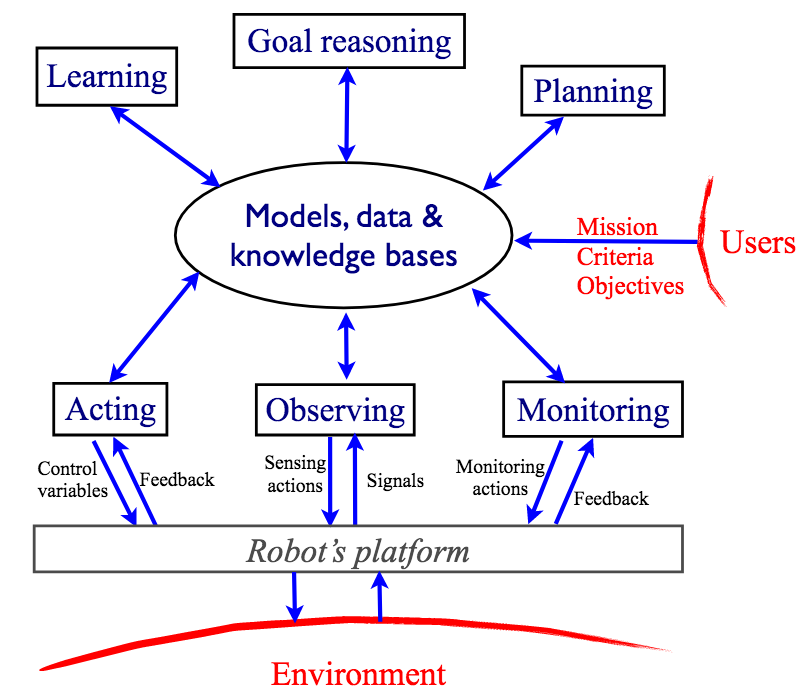
\includegraphics[scale=0.50]{figures/deliberationfunctions}
	\caption{Schematic view of deliberation functions \cite{ingrand2017deliberation}}
	\label{fig:deliberationfunctions}
\end{figure}

The framework that we propose with this project allows users without any programming knowledge to teach a robot a goal-oriented behaviour. 
Unlike current PbD implementations, which teach the robot an action sequence to achieve a goal, we want to equip the robot with all actions required to generate the action sequence autonomously using automated planning techniques. The user needs to construct a planning domain, consisting of all actions that the user taught the robot by demonstration.
 Using this knowledge base, the user can define a planning problem, for which the robot will generate a plan.
 PbD implementations using Hidden Markov Models recognise examples from training sets and use probabilities to assign an action.
 This requires training sets that are large enough to cover a wide range of possible world states.
 With our goal-oriented approach, the robot can solve an infinite number of goals, by using a limited set of actions.
 Figure \ref{fig:framework} shows the layout of our proposed framework (user activities are shown in blue and robot activities are shown in red).
 

  \begin{figure}[!h]
    \centering
    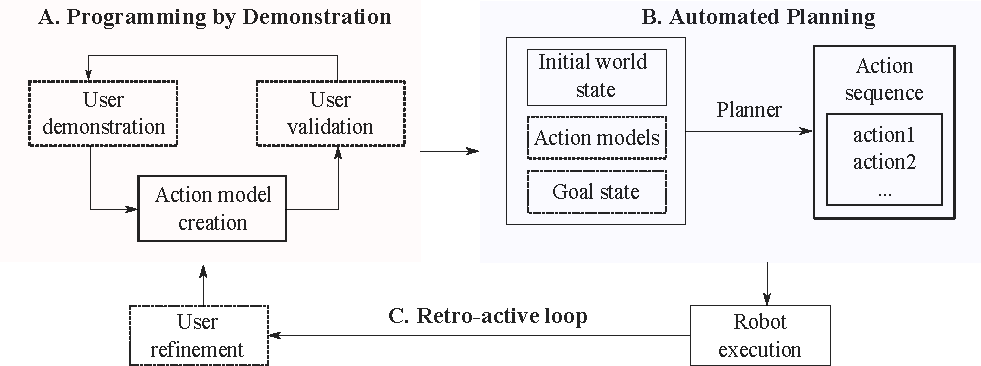
\includegraphics[width=\linewidth]{figures/framework}
    \caption{Framework for Robot Programming by Demonstration}
    \label{fig:framework}
  \end{figure}

\section{Creation of the Knowledge Base}
The user (in blue) interacts with the robot (in red) using a graphical interface.
The user has to create the planning domain, as specified in \sect{subsec:Planning domain description}, by defining the requirements, object types and predicates, i.e. conditions that can be included in the action definition.
The graphical interface should present the PDDL definitions in English sentences for the user.
Note that the object type definition at this stage is only at a syntactical level.
The instantiation of the locations and objects only occurs in the problem definition.
This leaves the user with the creation of the action models.

The actions will be created sequentially by iteratively providing demonstrations of the each individual action.
The robot extracts the relevant information from the demonstration using its sensors and builds a model of the learned skill.
By observing the changes in the state of the world, the robot suggests preconditions and effects, selected from the domain description, to be associated with the taught action.
After each demonstration, the user is presented with options to reproduce the learned skill or to modify the observed conditions.
The user either validates the learned action or provides another demonstration to refine it.
 

The action can be learned by generalising over a set of trajectories and by using statistical learning techniques, to deal with uncertainty contained in multiple motion demonstrations (\cite{ude1993trajectory}).
Once the user is confident about the created action model and its associated conditions, they can save it to the knowledge base.
 This process is repeated for all action models that are required to build the knowledge base for the complex task.
 The action models are automatically translated into PDDL, allowing the creation of a PDDL domain, without the requirement for any programming knowledge.

\section{Task Execution}
The created knowledge base is internally connected with a planner.
 The user needs to create a planning problem, as specified in \sect{subsec:PPDescription}, by listing all objects of the planning problem.
 To associate the PDDL objects with the physical objects in the real world, the user needs to assign features to each object in the planning problem, to allow their easy recognition.
 For instance, the robot can learn to recognise objects by their colour or shape, and locations can be saved using their end effector coordinates.

Instead of defining the initial state, the robot should recognise it using its sensors, allowing the user to verify the robot's learned object recognition.
 Once the planning problem has been defined, the robot can generate a plan.
 The action sequence will then be executed by the robot in order to achieve the goal state.
 If the user changes the goal, a new plan will be generated accordingly.
This removes the intermediate step of having to define an action sequence manually every time the goal changes.
 
If the proposed solution is not optimal, the user can modify them or refine the action models.
 Missing predicates in the action definition can lead to suboptimal solutions.
 The generation of an action sequence provides the user with the opportunity to test the soundness of their created action models.\\

\noindent In summary, our proposed framework links techniques from the two disciplines Programming by Demonstration and Automated Planning to create a means for the non-expert user to teach a robot a goal-oriented behaviour.
 The user's steps can be summarised as follows:

\begin{enumerate}
\item Define the requirements, types and predicates for the domain description.
\item For all actions:
\begin{enumerate}
\item Record an action demonstration for the robot learner.
\item Verify the derived policy and validate the proposed preconditions and effects.
\item Optionally provide additional demonstrations to refine action.
\end{enumerate}
\item Define a planning problem using the created domain, including a goal state.
\item \textit{The robot recognises the initial state and generates a plan.}
\item Verify that the action sequence of the plan is correct.
\item Optionally refine the created action models.
\end{enumerate}

\cleardoublepage
\chapter{Pre-Experiments}\label{chap:Pre-Experiments}
\minitoc

%%%%%%%%%%%%%%%%%%%%%%%%%%%%%%%%%%%%%%%%%%%%%%%%%%%%%%%%%%%%%%
%\section{Basic Research Questions and Their Evaluations}
\label{sec:hypotheses}

In the previous chapter (\chapt{chap:Contribution}) we proposed an end-user robot programming framework that allows users to teach robots new actions by demonstration, that can be reused with automated planners to complete previously unseen tasks.
We believe that non-robotics expert users without experience in automated planning can easily learn to use this framework.
Thus, %to evaluate the framework's usability for non-expert users, 
%we formulated the following hypotheses
%\begin{enumerate}
%\item[\textbf{H1}] \textit{The user understands the symbolic planning concepts.} This allows us to verify, if the symbolic planning language (PDDL), to describe the world state in terms of object types, properties, generalised properties, and action models, in terms of preconditions and effects, can be adopted easily by non-expert users.
%\item[\textbf{H2}] \textit{The user is able to teach the robot an action model using the proposed framework.} This allows us to evaluate how users operate the framework.
%\end{enumerate} 
we conducted two qualitative user experiments to respond to the following questions:
\begin{enumerate}
  \item[\textbf{Q1}] How do non-expert users adopt the automated planning language with its action model representation? (Section \ref{sec:Exp1})
  \item[\textbf{Q2}] Can users teach a robot action models for automated planning using the robot programming framework? (Section \ref{sec:Exp2})
\end{enumerate}

The experimental context was designed around a Baxter robot (\fig{fig:Baxter}).
In both experiments we included elements to assess the user's understanding of action models used by automated planners.
Understanding this symbolic representation is a key requirement to use the proposed framework.
In the following sections we briefly outline the experimental setup, measurements and results for each experiment.
 
% \begin{table}[t]
% \caption{Description of the world state in PDDL}
% \label{pddl_deschription}
% \begin{center}
% \begin{tabular}{l|l|l|l} \hline
%  \textbf{object name} & \textbf{type} & \textbf{property} & \textbf{generalised property} \\ \hline 
% redCube & cube & (at cube A) & (at ?cube ?posA)\\ \hline 
% A & position & (empty A) & (empty ?posA)\\ \hline 
% \end{tabular}\label{tab:pddl_deschription}
% \end{center}
% \end{table}

% Taken from Paper2 Basic research questions + experiments 1

\section{Experiment 1: Acceptance of Automated Planning and PDDL Concepts}\label{sec:Exp1}

% \section{How do non-expert users adopt the automated planning language with its action model representation?}
%%%%%%%% 1.25 pages %%%%%%%
In this experiment, we are addressing the following question:

\begin{enumerate}
	\item[\textbf{Q1}] How do non-expert users adopt the automated planning language with its action model representation?
\end{enumerate}

Users were introduced to a symbolic planning language (a simplified version of PDDL), involving the STRIPS formalism (\cite{fikes1971strips}) with type structures used in automated planning (\chapt{chap:Sota-AP}).
Users were instructed to describe world state configurations to the robot.
The goal was to assess the user's adoption of the planning concepts (object types, properties, generalised properties, action models) and to verify that the symbolic planning language is appropriate for non-expert users.

\begin{figure}[htp]
	\centering
	\begin{subfigure}[t]{0.24\textwidth}%
		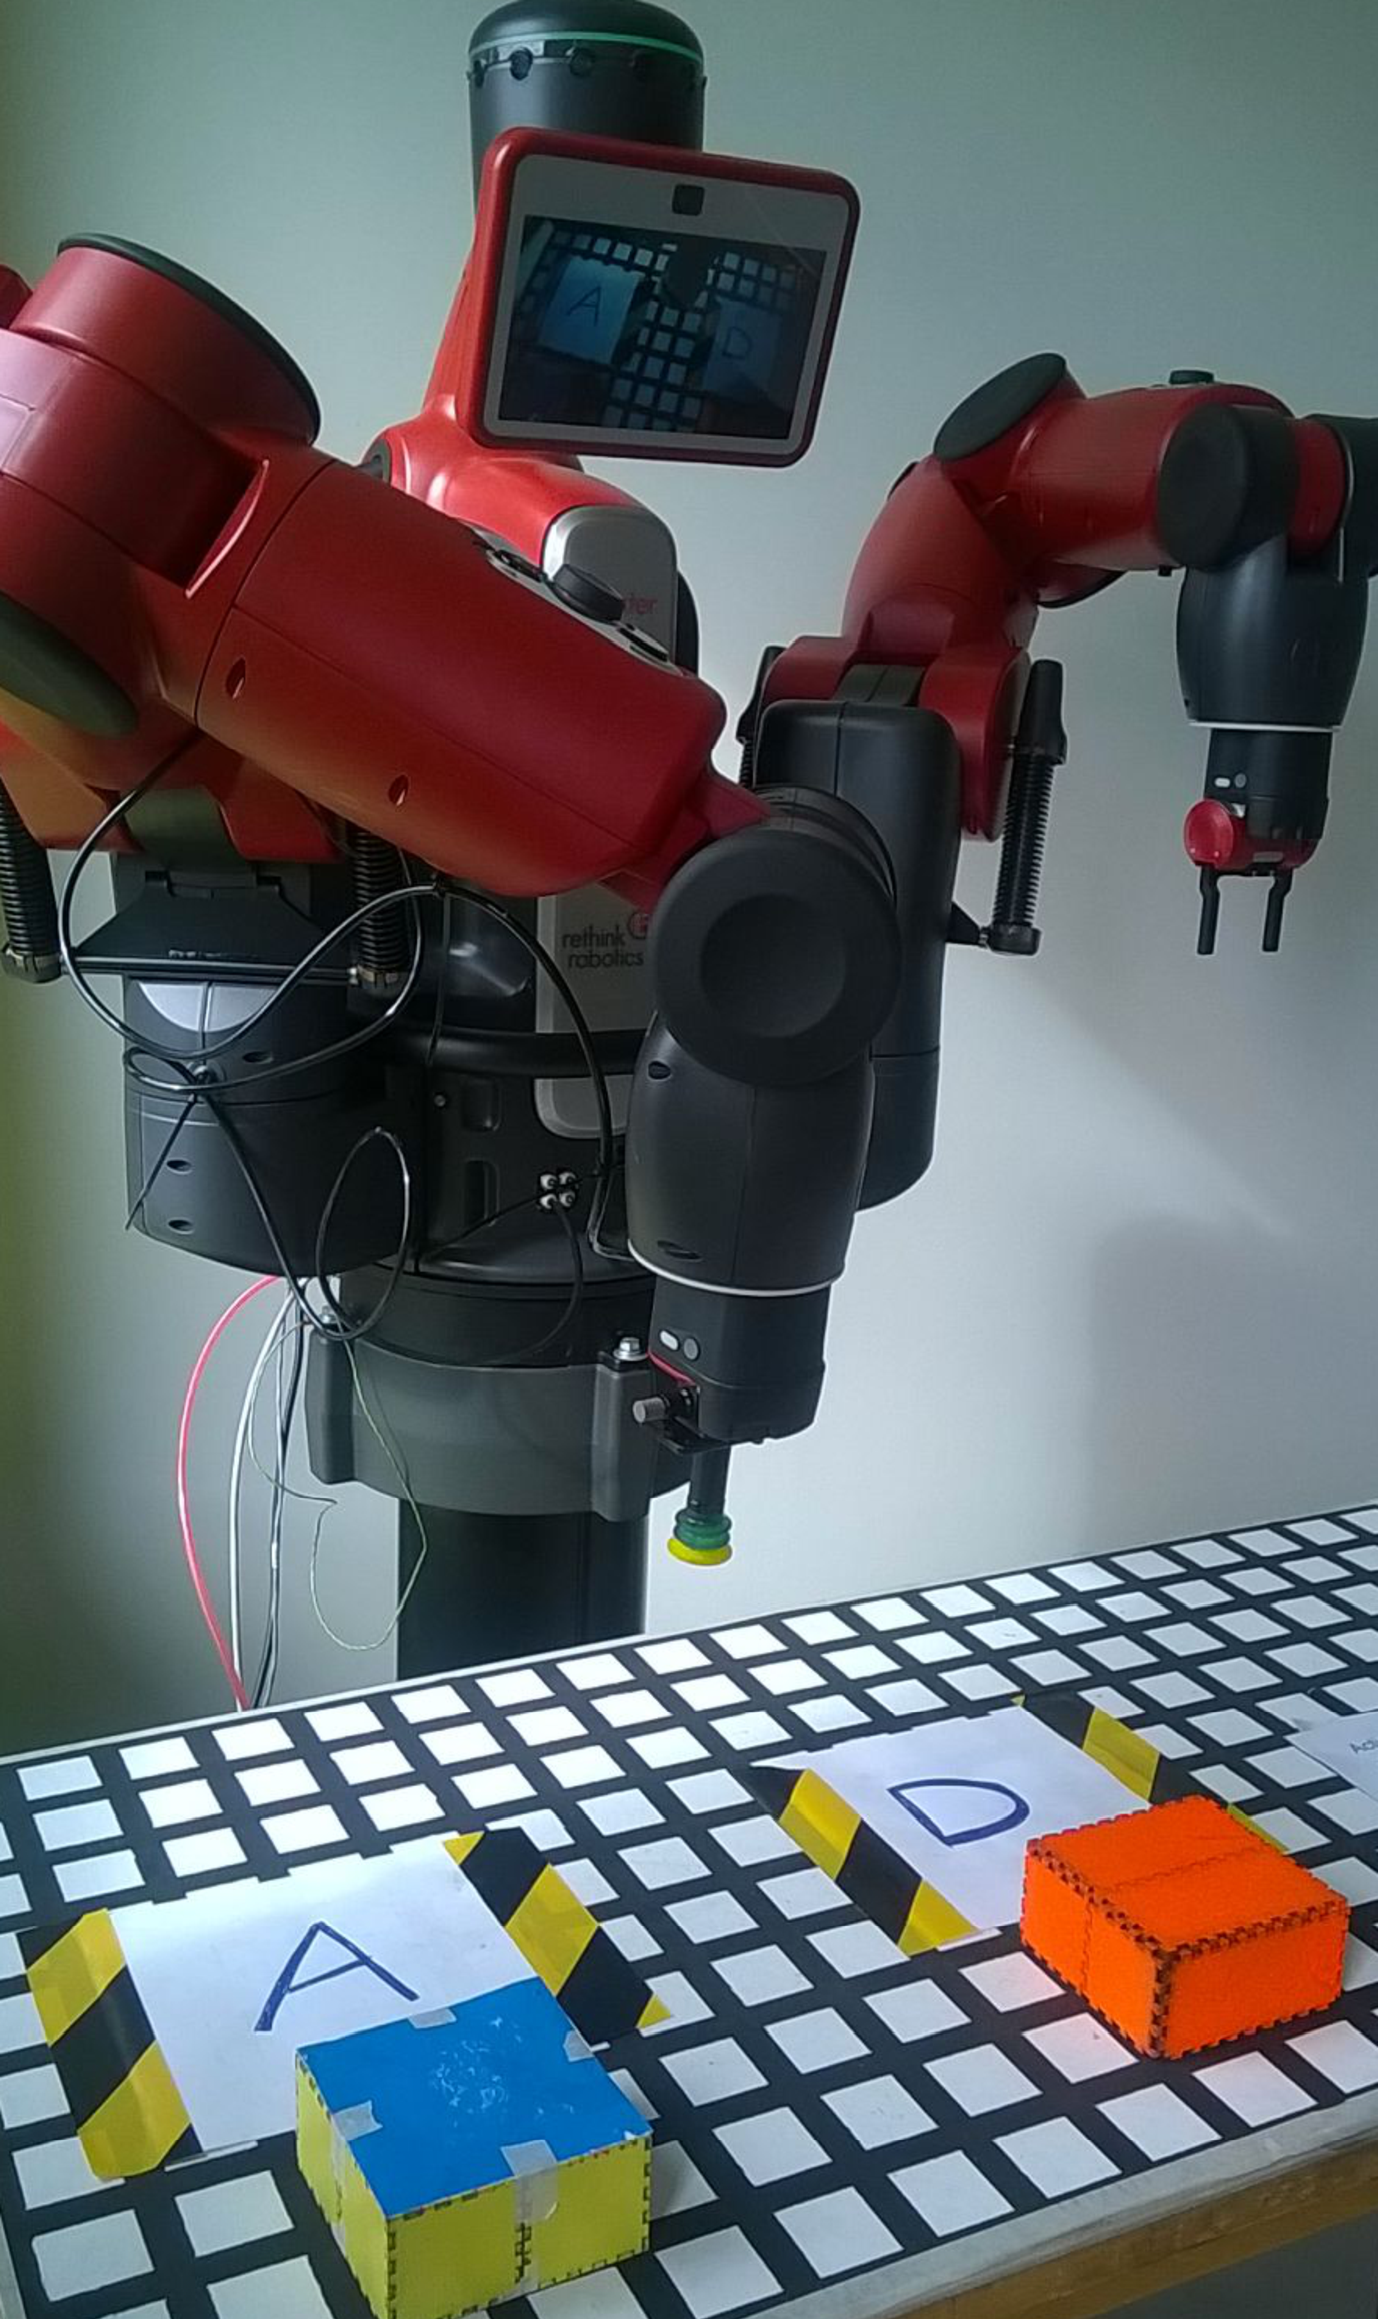
\includegraphics[width=\textwidth]{figures/experiment1}%
		\caption{Baxter robot}\label{fig:Baxter}%
	\end{subfigure}~~%
	\begin{subfigure}[t]{0.24\textwidth}%
		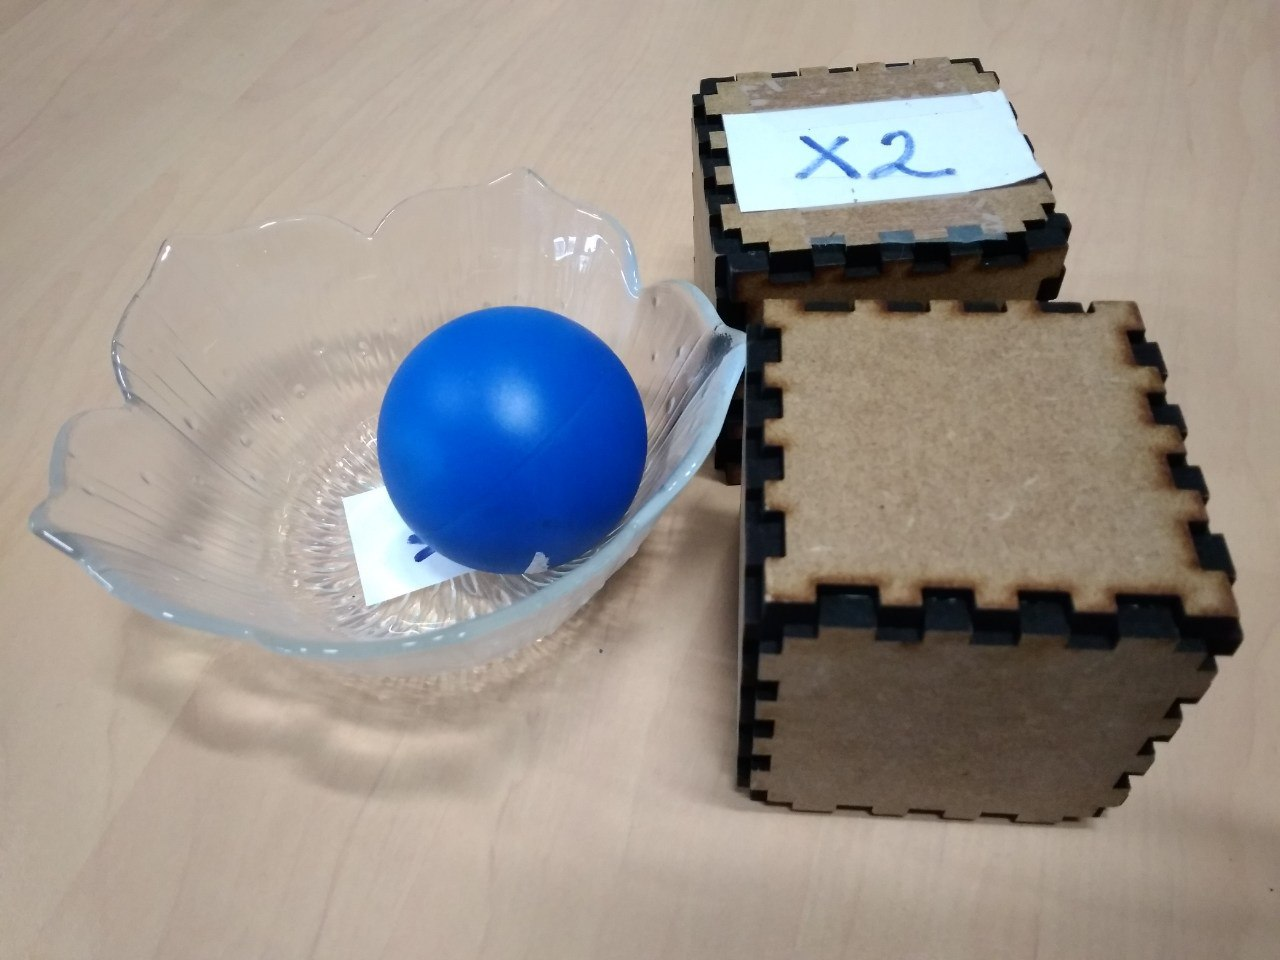
\includegraphics[width=\textwidth]{figures/exp1-setup}%
		\caption{Experiment 1 setup}\label{fig:exp1-setup}%  
	\end{subfigure} 	  
	\caption{Experimental setup for user studies.}
	\label{fig:pre-experiment}%
	% 	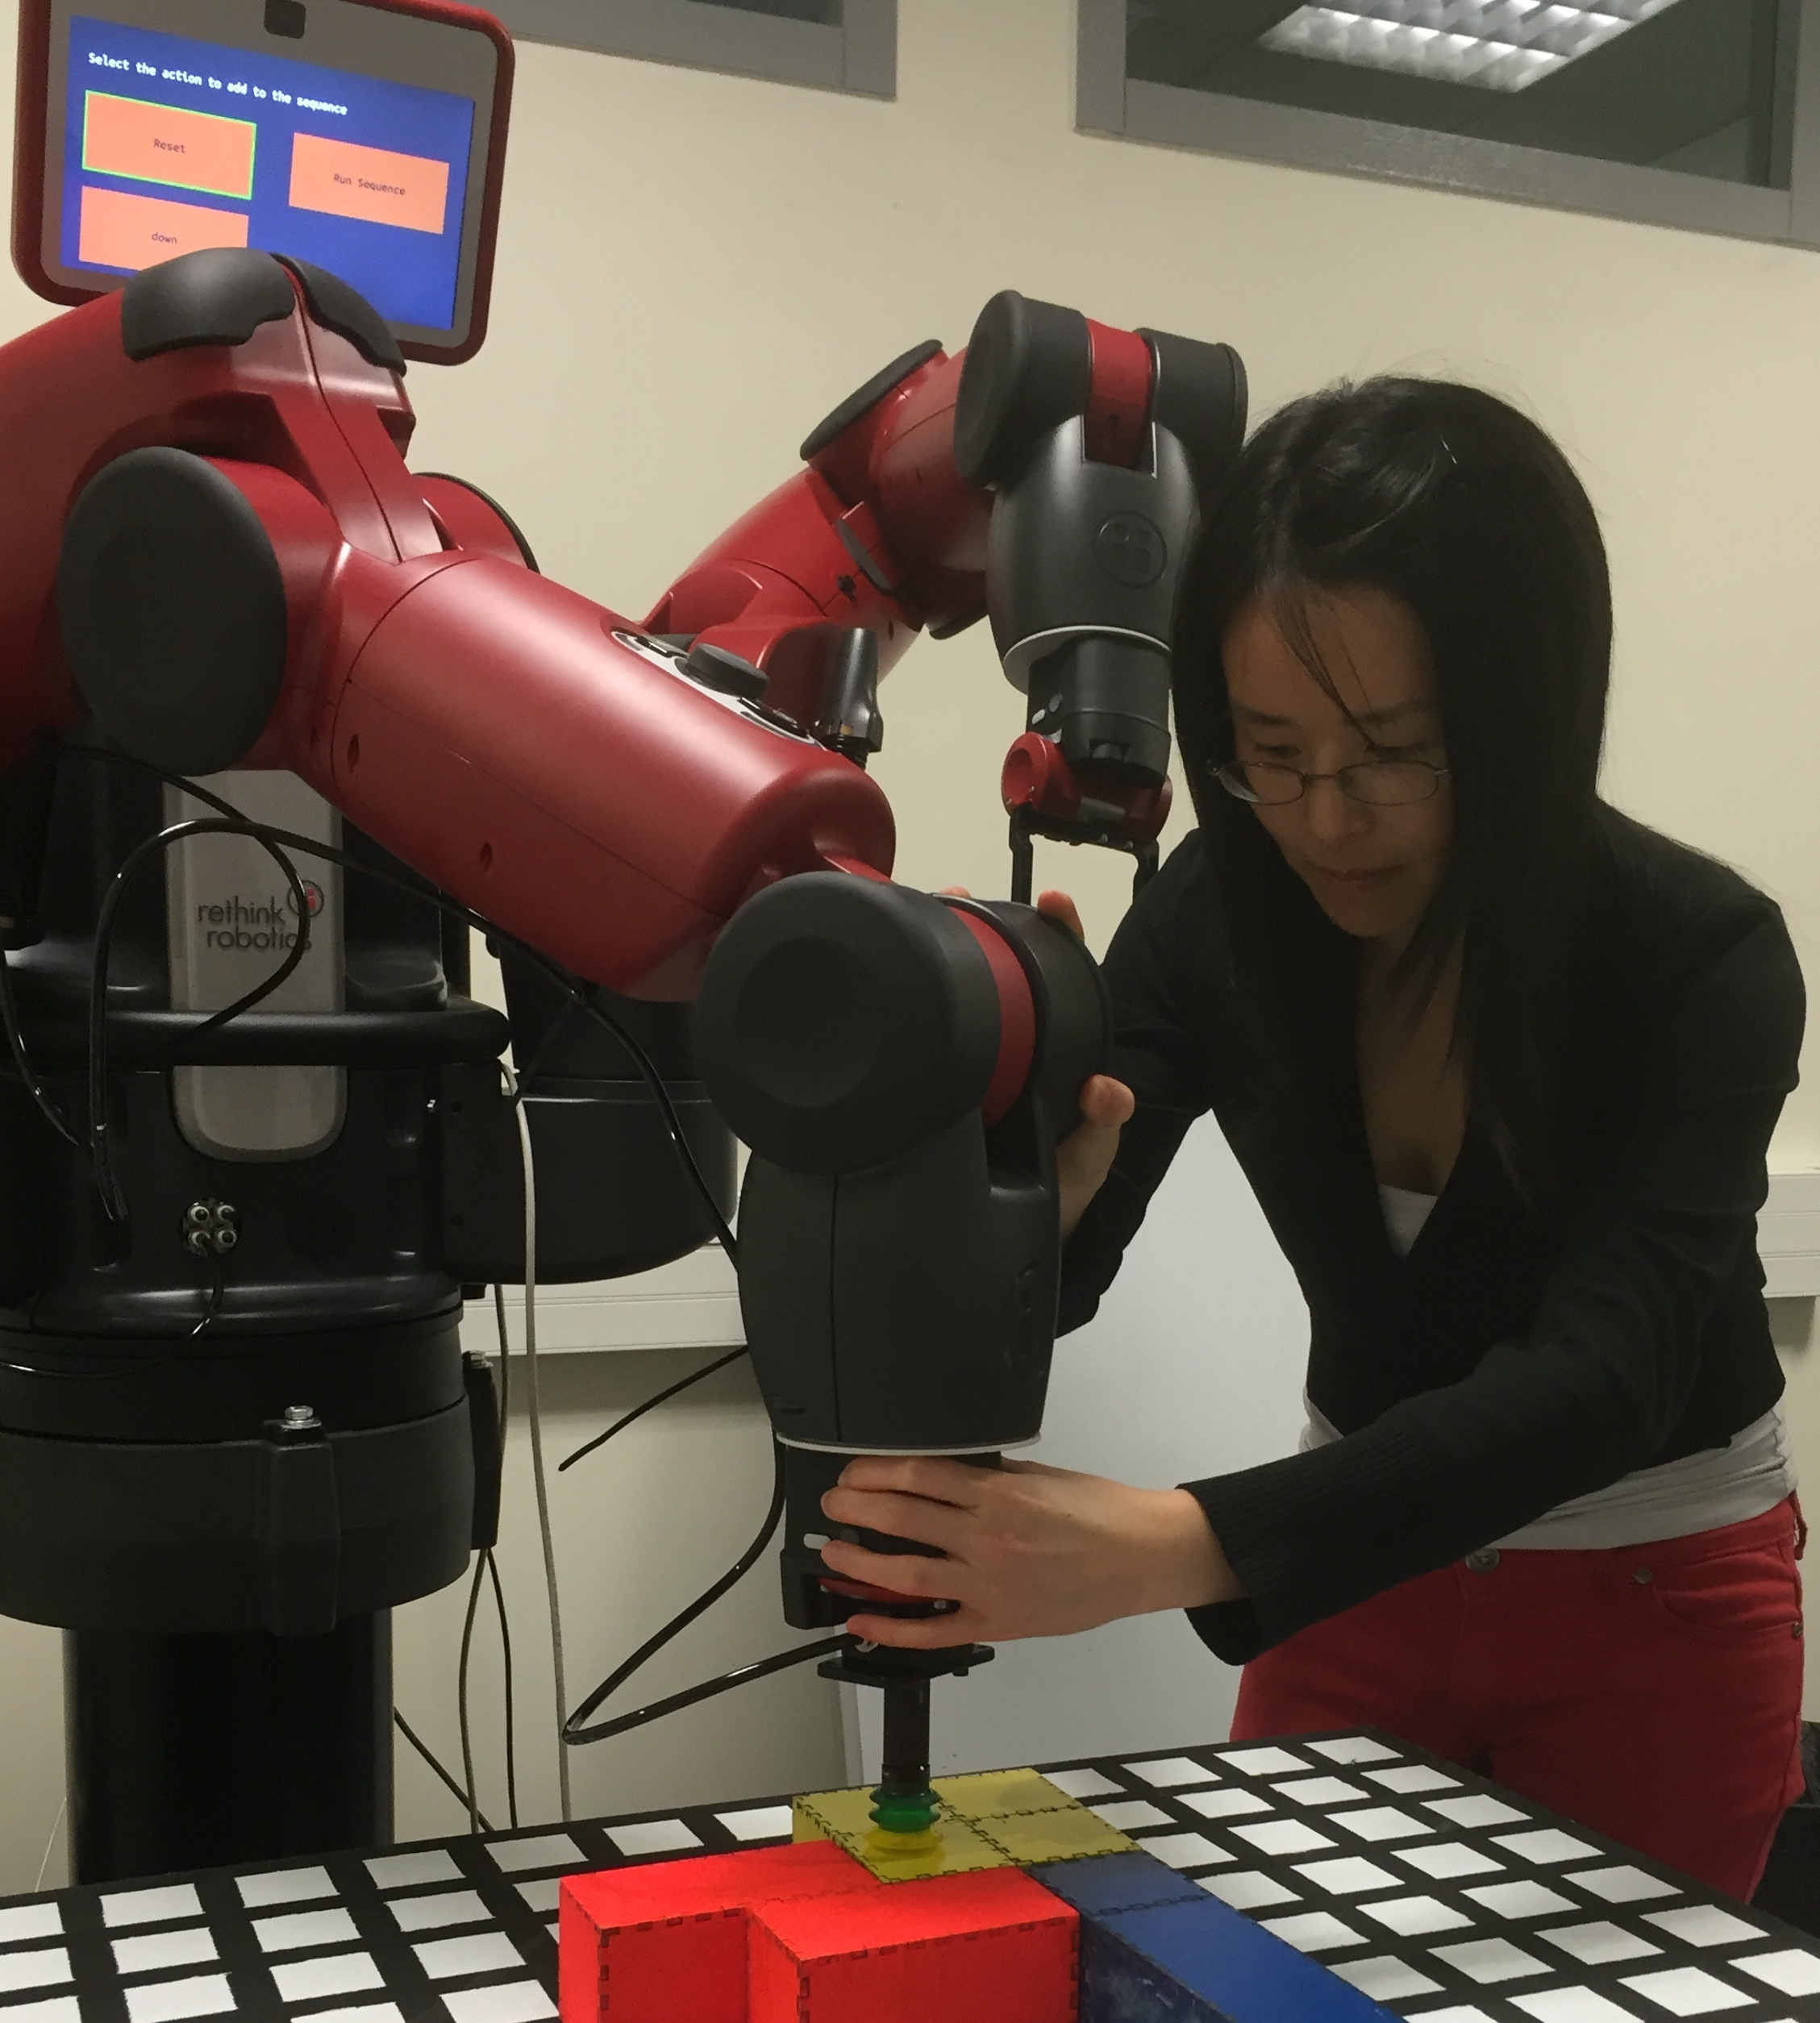
\includegraphics[width=.3\textwidth]{figures/experiment-setup2}
\end{figure}
\subsection{Experimental Setup \& Participants}
We recruited 10 participants (1 male, 9 female), who were sociology students at the Universit\'{e} Grenoble Alpes.
3 participants reported no programming experience, 6  had experience with office productivity software (`beginner'), and 1 had previously taken a programming course before (`advanced').

The experimental setup consisted of a 2x2 board (with positions A1, A2, B1, B2), 2 cubes, 1 ball, and 1 ball recipient in the form of a bowl (\fig{fig:exp1-setup}).
%The experimenter showed the participants a video of the Baxter robot \cite{Baxter}
The participants were given sheets with empty tables to complete for each task.
Each participant was allocated 1 hour, but the average duration of the experiment was 49 minutes.
At the end, participants were given a questionnaire related to their experience and their understanding of the learned planning language and concepts.
The participants' behaviour was observed by the experimenter and the experiment was recorded on camera.
The experimental protocol, questionnaire and additional material used can be found in Appendix \ref{app:exp1}.


%\begin{figure}[h]
%	\centering
%	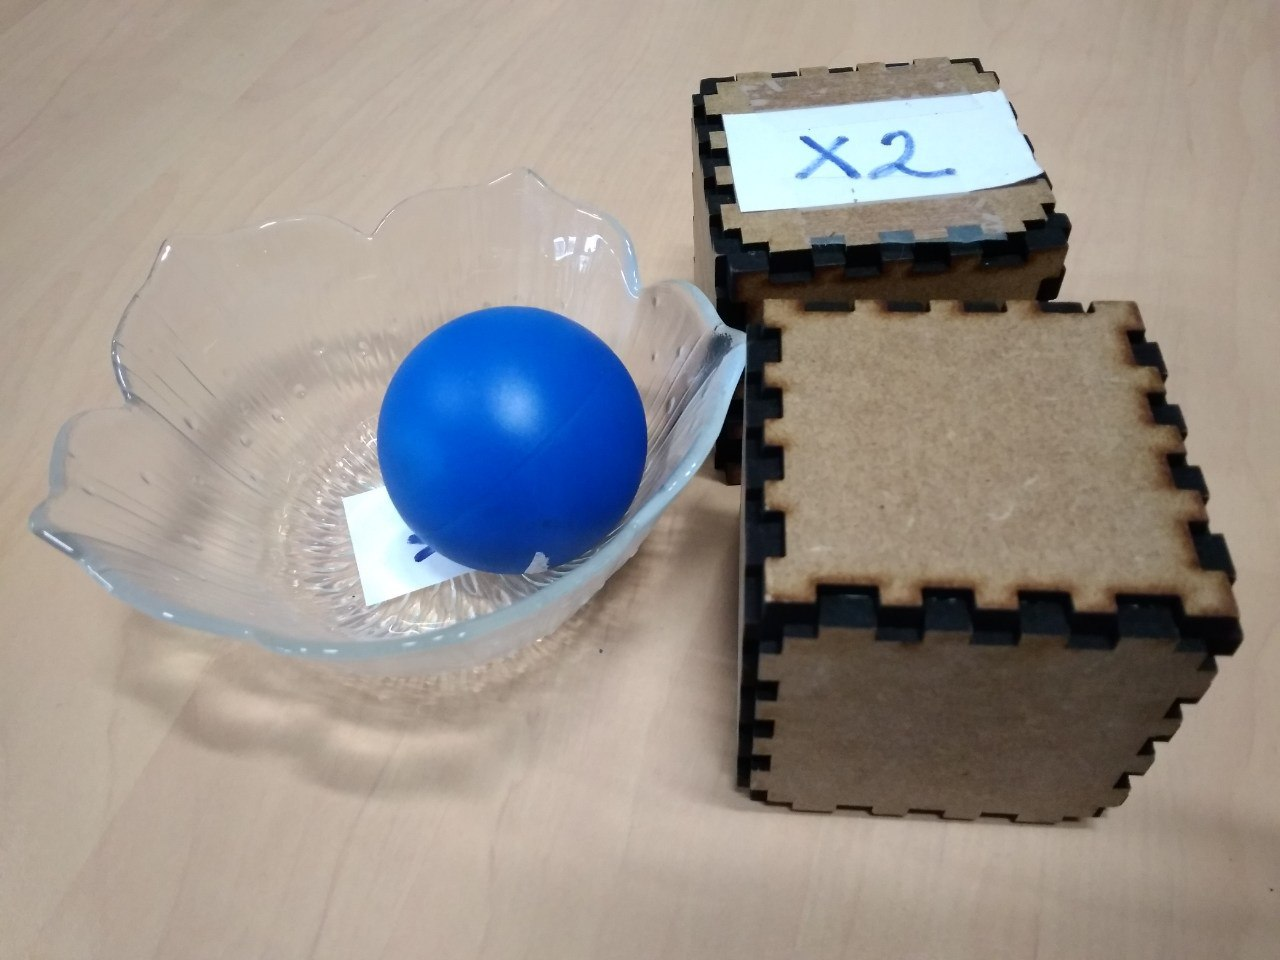
\includegraphics[width=0.65\linewidth]{figures/exp1-setup}
%	\caption{Experiment 1 setup consisted of a 2x2 board, 2 cubes, 1 ball, and 1 ball recipient}
%	\label{fig:exp1-setup}
%\end{figure}
 

\subsection{Experimental Design \& Measurements}
%After a short introduction to the Baxter robot, 
Users were told that they needed to use a symbolic planning language to describe the state of the world and the semantic meaning of actions to the robot. 
Throughout the experiment, users were faced with three different scenarios. 
\fig{fig:scenarios-exp1} shows an example of the experimental design, where the robot's action was to move the ball to an occupied position (B2). 
We evaluated their capability to apply the planning language to different situations.

\begin{figure}[h]
	\centering
	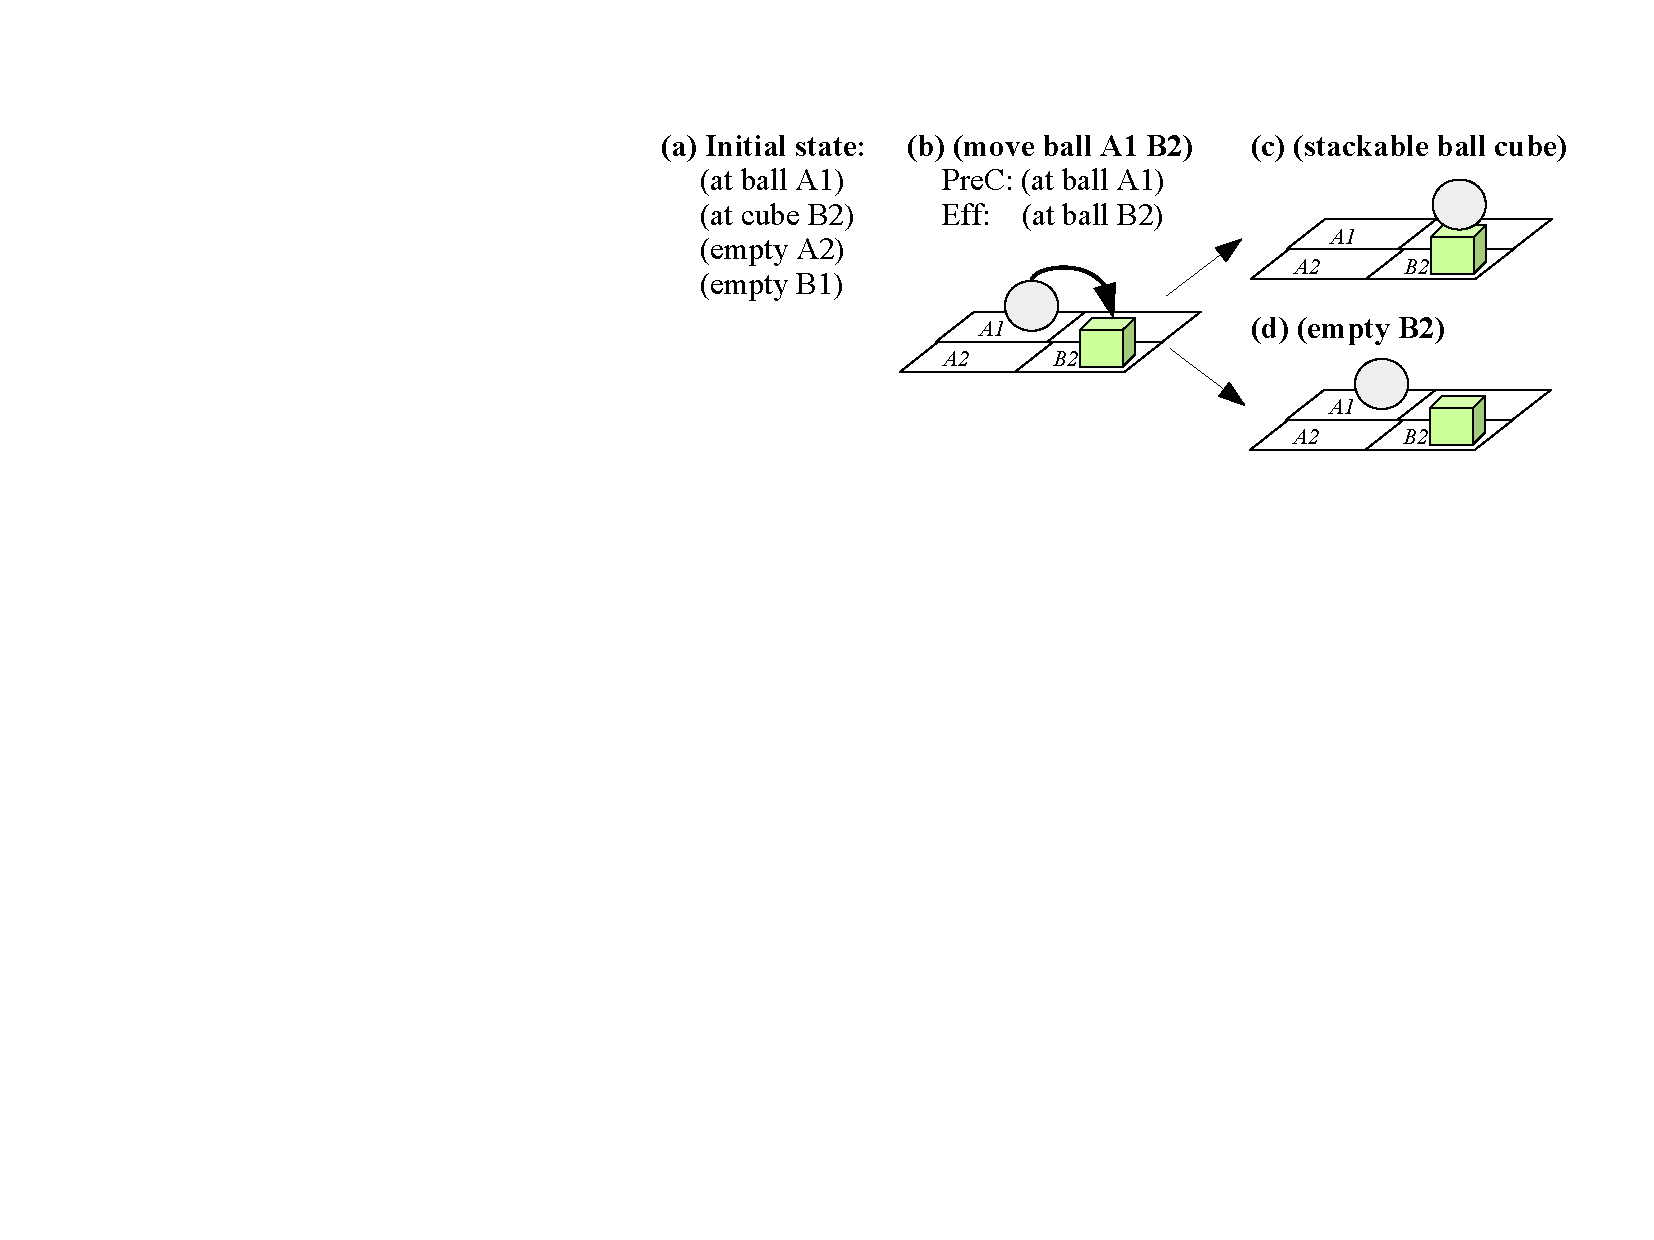
\includegraphics[width=0.75\linewidth]{figures/scenarios-exp1}
	\caption{Users were instructed to provide a description of (a) the initial state of the world and (b) an initial move action model.
		Then they derived additional preconditions for moving the ball from position A1 to B2: (c) \textit{(stackable ball cube)}: the ball can be stacked onto the cube, and (d) \textit{(empty B2)}: if the ball cannot be stacked, the target position should be empty.}
	\label{fig:scenarios-exp1}
\end{figure}

The experiment consisted of the following phases:
\begin{itemize}
%  \item{Introduction: After a short introduction to the Baxter robot \cite{Baxter}, users were told that they needed to use a planning language (STRIPS) to explain Baxter the state of the world and the semantic meaning of the actions.}
  \item{\begin{sloppypar} \textbf{Training:} Users were presented the symbolic planning language to describe object \textit{types} (\ie position, ball, cube, bowl) and predicates, which we called \textit{properties} (\ie \texttt{empty}, \texttt{at}, \texttt{stackable}, \texttt{is\_red}, \texttt{is\_blue}) to describe world states.
They were shown how to model a simple move action in terms of preconditions and effects (\fig{fig:action model}).
For all properties and actions, they had to use syntax of the form \texttt{name(arg1,arg2,\dots)} which users without a  Computer Science background might be unfamiliar with.
Additionally, they were introduced to the concepts of \textit{instantiated} and \textit{generalised} actions, which were equivalent to actions (\eg \texttt{move(X1)}) and planning operators (\eg \texttt{move(cube)}) respectively (\sect{subsec:Classical planning problem}).
In this phase, they were given a simple example of a cube at position A1 and moved to position B2.\end{sloppypar}
}
  \item{\textbf{Experimental test:} Users were presented a new world state that involved a cube, a bowl and a ball object. 
  	First they were instructed to provide a description of the initial state to the robot by using the symbolic planning language (\fig{fig:scenarios-exp1}a).
Then they were asked to define a move action model in terms of preconditions and effects (\fig{fig:scenarios-exp1}b).
In the following they were faced with 3 different scenarios to refine the preconditions of the move action.
Users derived a \texttt{(stackable ball cube)} property (\fig{fig:scenarios-exp1}c), which allowed a ball to be stacked on top of a cube.
When this property did not hold, users proposed the \texttt{empty} property (\fig{fig:scenarios-exp1}d), which the robot needed to verify before the action execution.
At each step, users had to give the generalised representation of the properties and action models.}
  \item{\textbf{Planning:} Users were presented a description of a new initial state of the world and a goal state.
They were asked to define an action sequence, that allows the transition from the initial to the goal state (similar to \fig{fig:planning-permutation}c), and explain their reasoning using the symbolic action model representation.
This optional test allowed us to further verify their understanding of the planning concepts, in particular action preconditions and effects.}
  \item{\textbf{Questionnaire:} At the end of the experiment users were given a questionnaire including 5 questions related to their experience, as well as 15 questions to evaluate their understanding of the learned planning language and concepts (\fig{fig:eEvaluation2}).
  For the latter, questions related to their understanding of the concepts presented at the start of the experiment (\eg `Explain the difference between the precondition and effect of an action'), syntax (\eg `Using the presented language, how do you describe the property \textit{cube X4 is on position B3}?'),
  %If move(CUBE) describes a move action, tick all statements that are true.
  logical reasoning 
  	(\eg `Is it possible to have \texttt{(empty A)} and \texttt{(at cube A)} in the same state?'), and other concepts (\eg `What is the generalised form of the given object property?').
  The complete questionnaire can be found in Appendix \ref{app:exp1}.}
   \item {\textbf{Debriefing:} Throughout the experiment, users were asked open-ended questions (\eg `What properties do you observe in the current world state?'), so that they were guided as little as possible and their responses were unbiased.
When the participant struggled to find an answer, the experimenter guided the participant in a possible direction (\eg `Why can the ball not be placed on the cube?').} 
\end{itemize}

\begin{figure}[ht]
	\centering
	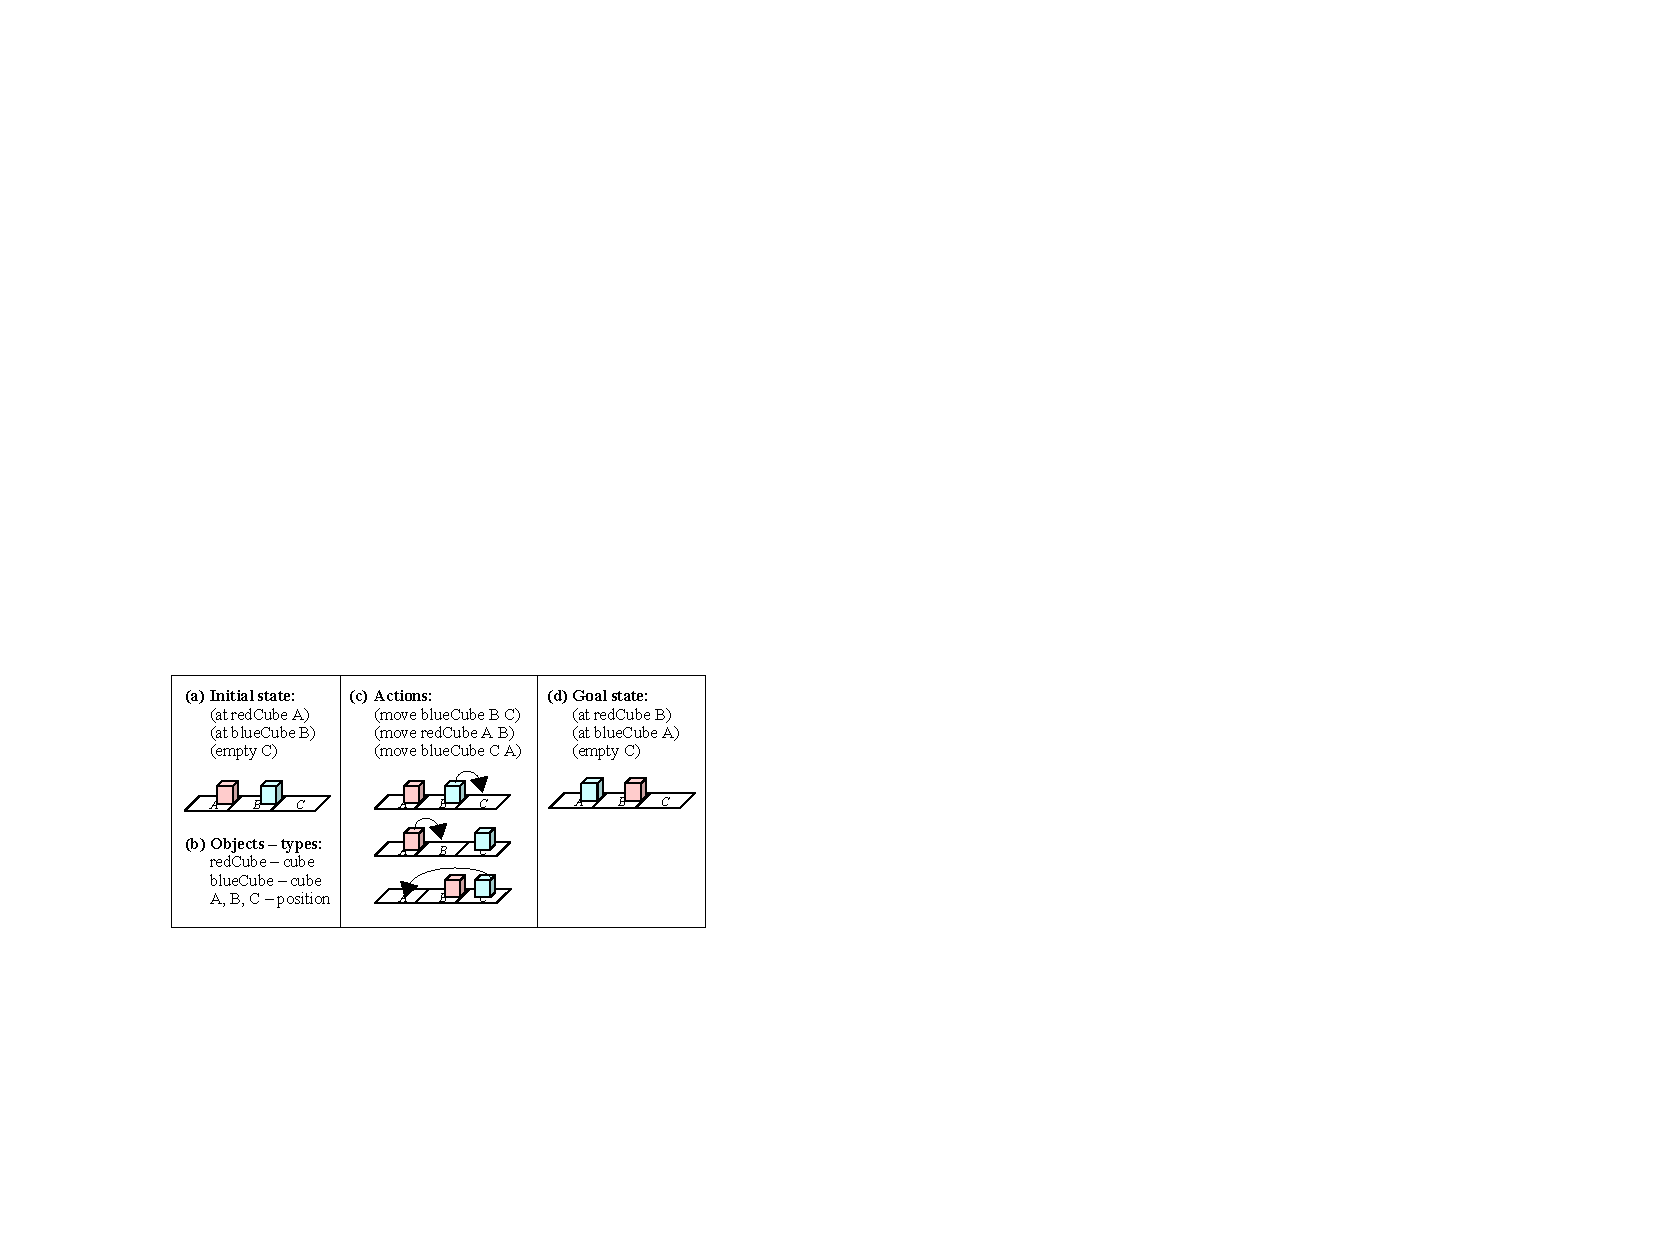
\includegraphics[width=0.7\linewidth]{figures/planning-permutation}
	\caption{Definition of a planning problem (a) properties describing the initial world state (b) object names and their types (c) instantiated actions (d) properties describing the goal state.}
	\label{fig:planning-permutation}
\end{figure}


\subsection{Results}
We did not observe any significant differences in the performance of users with or without programming experience.
9 (out of 10) participants found the symbolic representation of properties and actions easy to understand.
During the experimental test, the majority (9 or 90\%) of the participants managed to describe the complete world state using the correct syntax.
When faced with different scenarios to refine the move action model, 5 (or 50\%) of the participants struggled to formalise the \textit{stackable} condition in the symbolic language.
They provided alternative formulations related to the cube's properties (\eg `if the cube can hold the ball').
However, once the condition was defined, the majority (8 or 80\%) of the participants had little to no difficulties generalising properties, \eg defining planning operators (\fig{fig:action model}).
Due to time constraints, only 5 (or 50\%) participants were presented the planning phase.
All 5 encountered no problems when defining the action sequence to achieve the given goal.

In the questionnaire (\fig{fig:eEvaluation2}), the majority (9 or 90\%) of the participants understood the notion of states and object properties.
8 (or 80\%) correctly pointed out two properties that could not exist in the same state (\eg \texttt{(empty A)} and \texttt{(at cube A)}).
All participants gave correct explanations for preconditions and effects of action models, and provided correct examples.
9 (or 90\%) participants encountered difficulties during the experiment, 6 (or 60\%) stated problems with formalising the language, especially at the beginning of the experiment.
Half of the participants believed that they could apply this language on their own.
No participants believed that an `expert' programmer was required to learn the symbolic planning language, but 7 (or 70\%) participants believed that the minimum requirement was a `beginner' programming level, while 3 (or 30\%) believed that no programming experience was required at all.


\begin{figure}[ht]
	\centering
	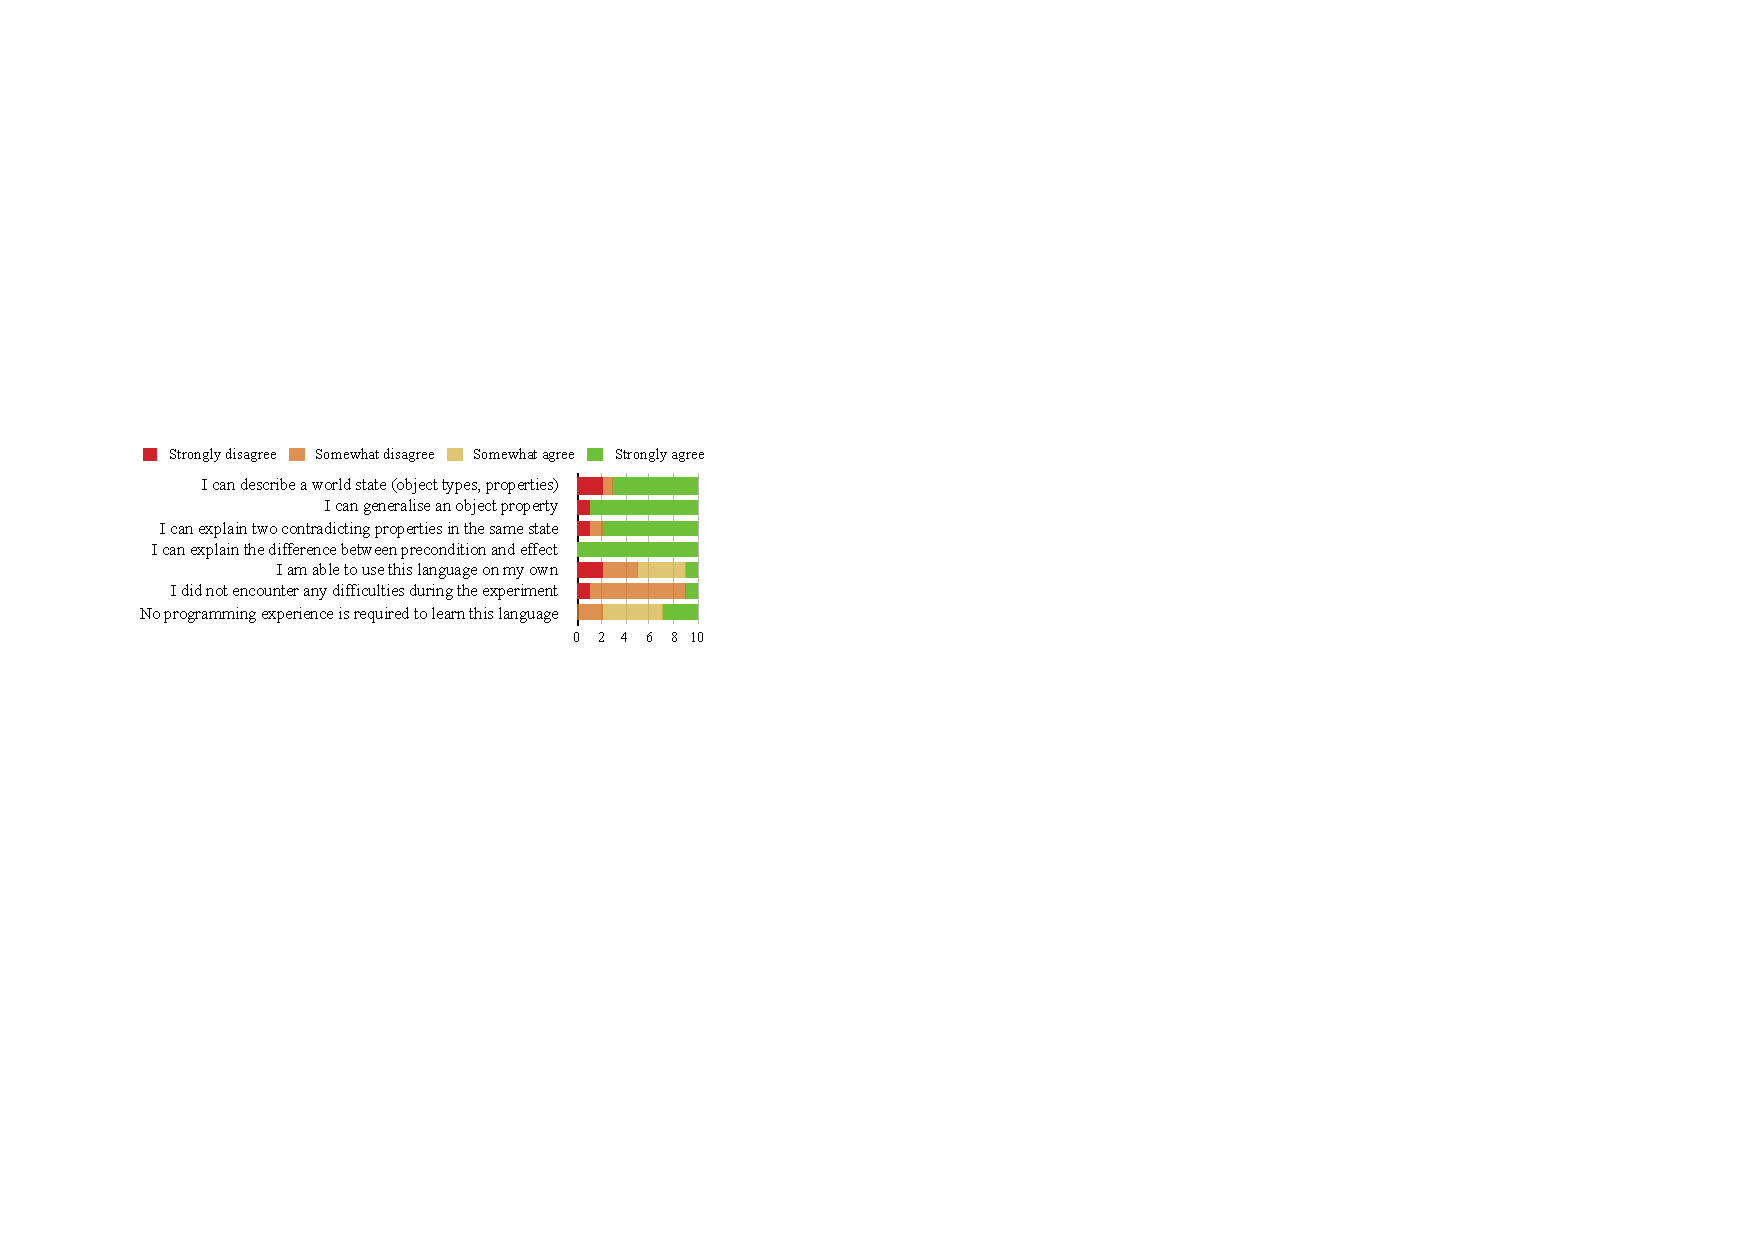
\includegraphics[width=0.85\linewidth]{figures/eEvaluation2}
	\caption{Summary of questionnaire responses: Extract of the 26 questions on the user's experience and understanding of the introduced planning language.}
	\label{fig:eEvaluation2}
\end{figure} 

\section{Experiment 2: Acceptance of the Robot Programming Framework}
\label{sec:Exp2}

In this experiment, we are addressing the following question:

\begin{enumerate}
  \item[\textbf{Q2}] Can users teach a robot action models for automated planning using the robot programming framework?
\end{enumerate}
\begin{sloppypar}
Users were presented a simulated implementation of the robot programming framework (\chapt{chap:Contribution}), and had to teach action models by kinesthetic manipulating a Baxter robot (\fig{fig:Baxter}). 
Users were instructed to demonstrate an atomic action and to assign preconditions and effects.
The goal was to assess the framework's usability and user's difficulties encountered when teaching action models.
At the end, participants were given a questionnaire related to their experience, their perceived understanding of the presented planning concepts and the usability of the framework.
The experimental protocol, questionnaire and additional material used can be found in Appendix \ref{app:exp2}.
In the following sections we briefly outline the experimental setup, measurements and results of the experiment.
%We then provide details on the partial implementation of the system used with the Wizard-of-Oz technique (\sect{ssec:WoZ}).
\end{sloppypar}

\subsection{Experimental Setup \& Participants}
We recruited 11 participants (7 male, 4 female), who were students and staff members at the Universit\'{e} Grenoble Alpes. 
6 participants reported programming experience with office productivity software (`beginner'), 2 had previously taken a programming course before (`advanced'), and 3 were pursuing studies in Computer Science (`expert').
%4 participants had previously heard of Automated Planning, but only 3 attended a related course.
The experiments were conducted using a Baxter robot (\fig{fig:Baxter}), mounted with a partial implementation of the framework.
The implemented functionalities included:
\begin{itemize}
	\item `learn new action': record the action demonstration
	\item `find a coloured object': apply the recorded action to an object of the specified colour
	\item `execute an action sequence': execute multiple actions
\end{itemize}

We used the Wizard-of-Oz technique to simulate the remaining functionalities (\eg `learn action preconditions and effects', `generate solution using a planner').
%Further details to the partial implementation are discussed in Section \ref{ssec:WoZ}.
Participants operated on a table with 2 positions D (for departure) and A (for arrival), 2 cubes (blue and red), that represented parts on an assembly line (\fig{fig:Baxter}). 
Each participant was allocated 1 hour, but the average duration was 29.5 minutes. 
The experiments were recorded, while the participant interacted with the robot. 


%The complete experimental protocol is shown in \fig{fig:Experimental protocol}. 
\subsection{Experimental Design \& Measurements}
The experiment scenario was set in a simulated assembly line, where objects of the same shape, but different colour arrived consecutively at the departure position D.
Users were told that objects were too heavy for human operators to move, hence needed to be handled by robots.
Also, due to the type of object, they should not be stacked.
Users had to teach Baxter the action for moving an object from D to arrival position A, for another maintenance task to be performed.
Throughout the experiment, users were faced with two different scenarios, where Baxter had to apply the learned move action. 
We evaluated the user's capability to refine action models and their associated conditions, when faced with different situations, and wanted to assess the framework's overall usability.

\begin{figure}[h]
	\centering
	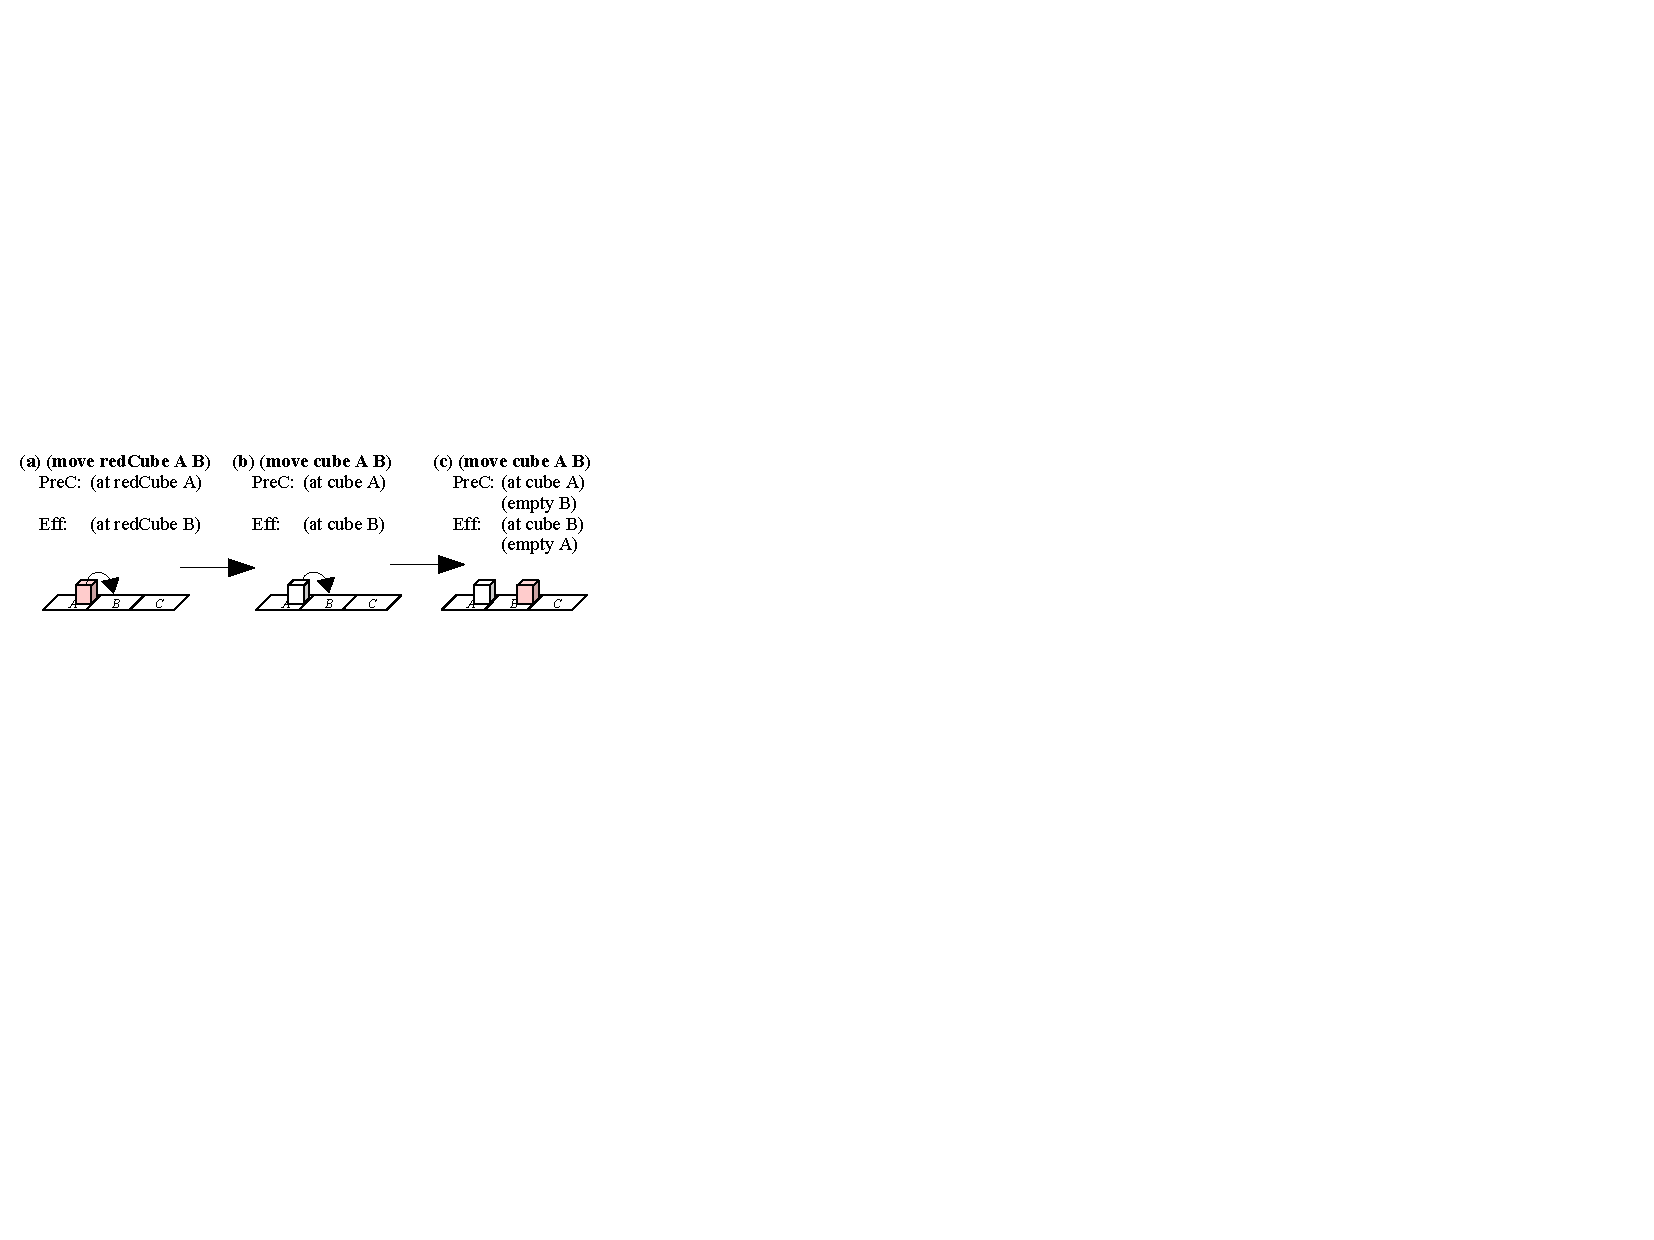
\includegraphics[width=0.8\linewidth]{figures/scenarios-exp2}
	\caption{Continuous refinement of the move action model: (a) initial action model learned by demonstration, (b) action model for all cubes of any colour, (c) action model with an additional condition, if the target position is occupied and cubes can not be stacked.}
	\label{fig:scenarios-exp2}
\end{figure} 

The experiment consisted of the following phases:
\begin{itemize}
  %\item{Introduction: After a short introduction to the Baxter robot \cite{Baxter}, users were told that they needed to use a planning language (STRIPS) to explain Baxter the state of the world and the semantic meaning of the actions.}
  \item{\textbf{Training:} Users were shown how to manipulate Baxter's arm, and given time to familiarise themselves with the kinesthetic manipulation. 
  	For this experiment we only used the robot's suction gripper to manipulate objects.}
  \item{\textbf{Experimental test:} Users were instructed to teach Baxter a move action of a red cube. 
  	Then, they were presented the action model, with preconditions and effects, that Baxter learned from the demonstration (\fig{fig:scenarios-exp2}a). 
  	In the following, users were faced with two different scenarios to refine the conditions of the action model. 
  	Starting with the initial action model for a red cube, users modified the conditions, so that it was applicable to all cubes of any colour (\fig{fig:scenarios-exp2}b), and when the target position was occupied (\fig{fig:scenarios-exp2}c). 
  	At each step, users observed how Baxter executed the learned action in the new scenario. 
  	When Baxter failed to execute the action, users had to refine the conditions of the action model.}
  \item{\textbf{Planning:} Users were presented a new scenario, where Baxter was instructed to achieve a goal using the learned action model. 
  	The new goal was to switch the positions of two cubes on the table (\fig{fig:planning-permutation}). 
  	Users first asked if they believed Baxter was able to solve this task and then shown how the taught action was reused with an automated planner.
  	Finally, Baxter executed the action sequence to complete the task.}
  \item{\textbf{Questionnaire:} Users were given a questionnaire containing 18 questions related to their experience (\eg `I did not encounter any difficulties during the experiment') and their perceived understanding of the presented concepts (\eg `I can explain how Baxter represented the preconditions of a new action'), and the usability of the framework (\eg `No programming experience is required to teach Baxter a new task').
  Participants had to give a rating on a scale ranging from `Strongly agree', `Somewhat agree', `Somewhat disagree', and `Strongly disagree'.
  The complete questionnaire can be found in Appendix \ref{app:exp2}.}
   \item{ \textbf{Debriefing:} Throughout the experiment, users were asked about their expectations on Baxter's behaviour before applying the learned action model to a new scenario. 
   	Users were asked open-ended questions (\eg ``What will Baxter do when applying the learned action model?"), so that their responses were unbiased. 
   	When they encountered failure scenarios (\eg when Baxter stacked two cubes), they were asked to reason about Baxter's behaviour and proposed modifications to the taught action model.} 
\end{itemize}

\subsection{Results}
During the experiments we observed how users learned and used the presented programming process and planning concepts.
When asked for improvements of the initial action model (\fig{fig:scenarios-exp2}a) no users pointed out missing conditions before being faced with the new scenario (\fig{fig:scenarios-exp2}c).
Even users who were `experts' and who have heard of automated planning before, did not propose a complete action model from the start. 
However, when faced with the relevant failure scenarios all users detected the missing conditions easily.
In the final phase, 8 (or 73\%) users with no experience in automated planning did not expect Baxter to solve the permutation problem, and agreed unanimously that it acted in an intelligent manner, when it did. 

Figure \ref{fig:eEvaluation} shows the user responses to the questionnaire.
All (11) users were satisfied with the PbD process and Baxter's abilities to learn and reproduce the demonstrated move action and no users encountered difficulties during the experiment. 
%All users understood the learned action model and managed to adopt the notions of preconditions and effects easily. 
At the end of the experiment, all users believed that they had taught Baxter a new task. 
The majority of users were confident that they could explain how Baxter learned and represented the new action model.
9 (or 82\%) understood the notion of preconditions and agreed that no programming experience was required to teach Baxter using the proposed framework.


\begin{figure}[h]
	\centering
	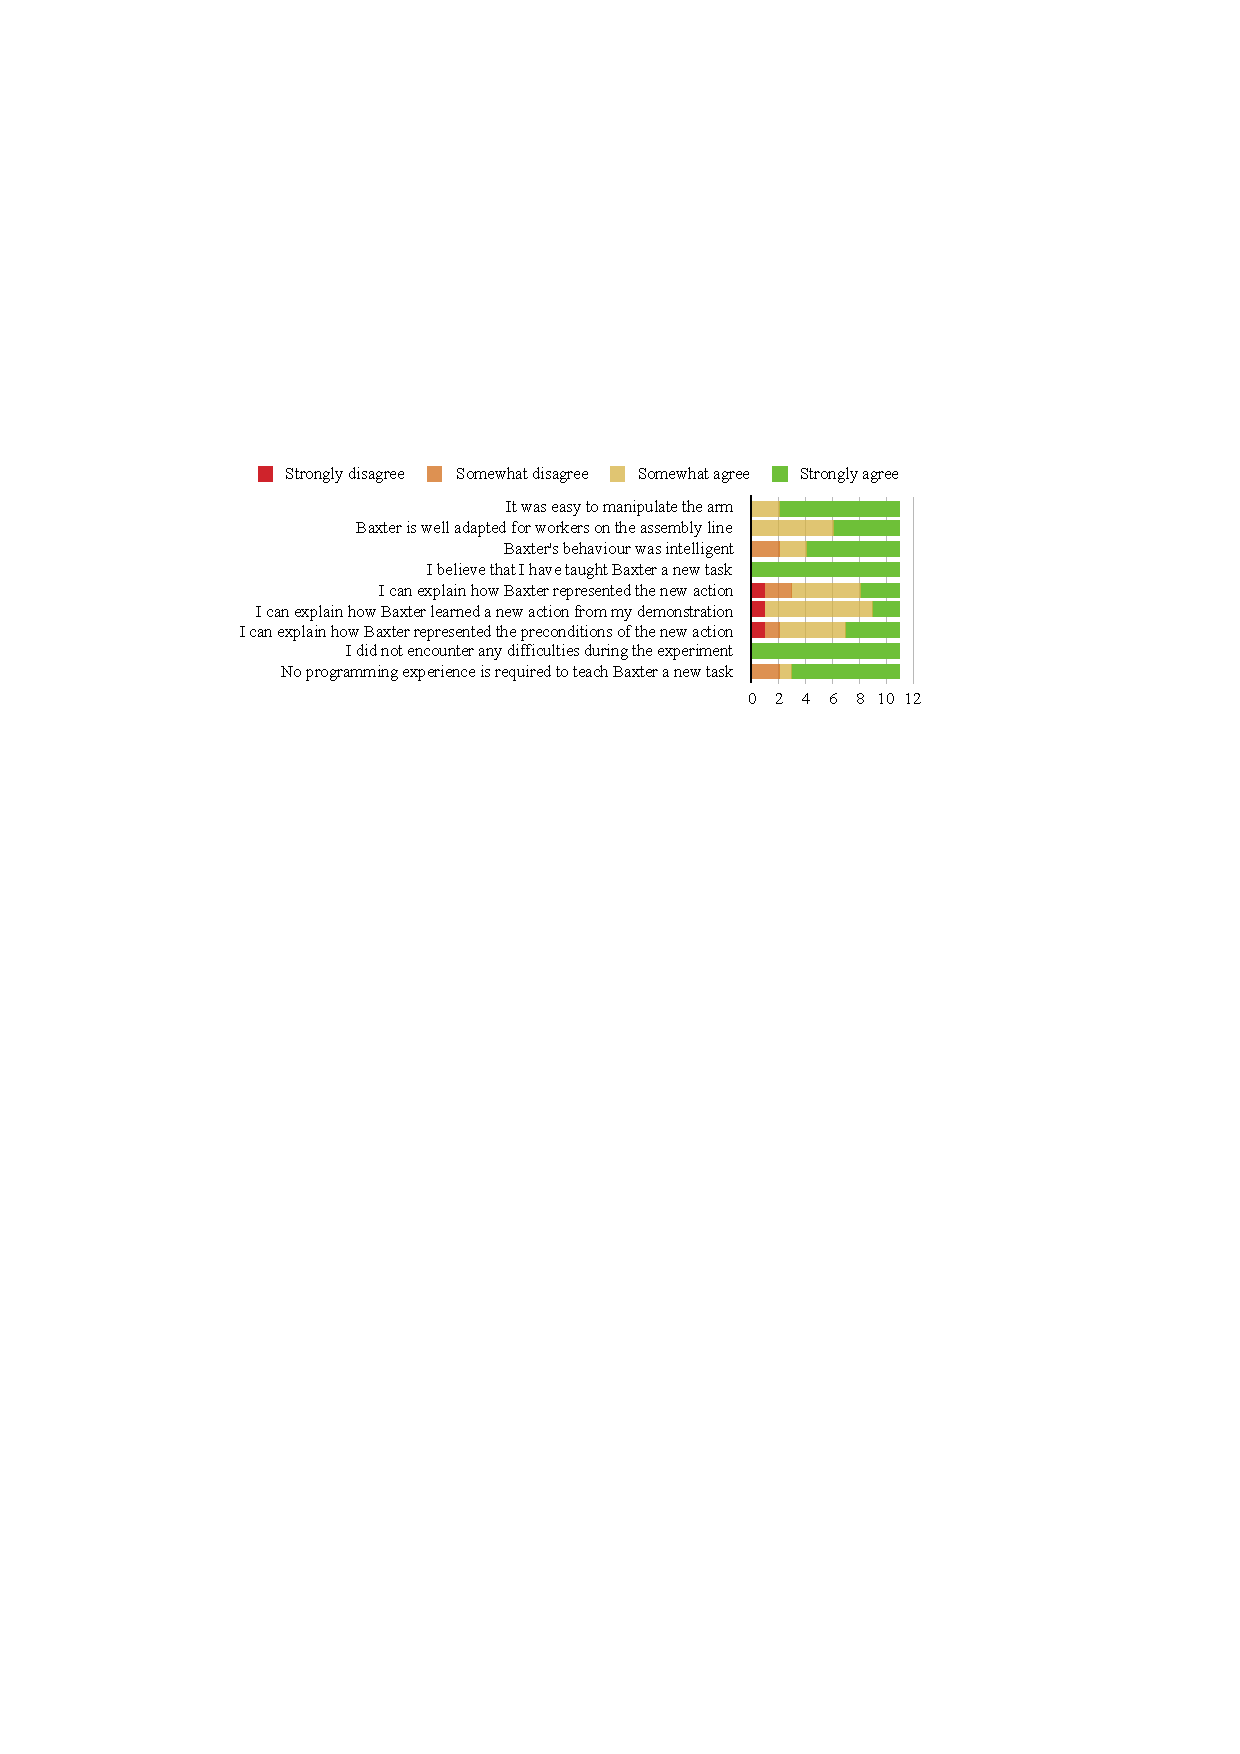
\includegraphics[width=\linewidth]{figures/eEvaluation}
	\caption{Summary of questionnaire responses: Extract of 18 questions on the user's perceived usability and understanding of the programming process after the experiment.}
	\label{fig:eEvaluation}
\end{figure}


\section{Discussion and Limitations}
In both experiments, we did not observe a significant difference in the performance between users with different programming experience. 
The majority of users had issues formulating the logical representations of object properties used in action models. In the first experiments, users had difficulties formulating a single condition (e.g. \texttt{(stackable ball cube)}), but stated equivalent conditions (\textit{`only place the ball, if it is stackable on the cube'}).
Similarly, in the second experiment, users formulated the missing precondition (\textit{`position B is empty'}) with other equivalent conditions (\textit{`Do not place the object on position B, if it is occupied'}). This means, that users should be provided with a predefined set of conditions that can be added to the action model.

Some users made wide assumptions about the robot's capabilities. In the second experiments, when both arrival and departure positions were occupied (Fig. \ref{fig:scenarios-exp2}c), less half of the users (5) expected Baxter to consider the occupied position, even though the condition was not mentioned in its action model.
This is a common problem in PbD solutions as there is a difference in the perception of the robot's intelligence perceived by its teacher (\cite{suay2012practical}) and can be addressed by reproducing the learned task in a new context and verifying the robot's knowledge base, as we did throughout the experiment.

With these two qualitative experiments, we showed that the automated planning language could easily be adopted by users without any programming background. Moreover, the action model representation, in terms of preconditions and effects, seems to be intuitive for non-expert users. 
However, these initial experiments only provide us with an idea of how the users might perceive the proposed framework. We intentionally limited the set of concepts that are necessary to use the framework to the bare minimum. Further experiments should test scalability and address more complicated actions involving separate control groups (experts vs non-experts) in less structured scenarios. 



\cleardoublepage
\chapter{Goal-Oriented End-User Robot Programming}\label{chap:OrganisingTasks}
\minitoc% Creating an actual minitoc
This chapter includes the most recent work in collaboration with Maya Cakmak, director of the Human-centered robotics Lab at the University of Washington.
Similar to the main challenge of this thesis, this work uses Programming by Demonstration to enable end-users to teach robots pick and place tasks.
The following paper has been submitted to IROS'2019 and is currently under review.
%\includepdf[pages=1-8]{iros-2018-simultaneous.pdf}


\cleardoublepage
\chapter{End-User Robot Programming for Task Planning}\label{chap:Implementation}
\minitoc% Creating an actual minitoc
This chapter includes the most recent work in collaboration with Maya Cakmak, director of the Human-centered robotics Lab at the University of Washington.
Similar to the main challenge of this thesis, this work uses Programming by Demonstration to enable end-users to teach robots pick and place tasks.
The following paper has been submitted to IROS'2019 and is currently under review.
%\includepdf[pages=1-8]{iros-2018-simultaneous.pdf}


\cite{ingrand2017deliberation} identifies six deliberation functions that are necessary to interface with robotic system to act autonomously: planning, acting, monitoring, observing, learning, and goal reasoning (\fig{fig:deliberationfunctions}).

\begin{figure}[h]
	\centering
	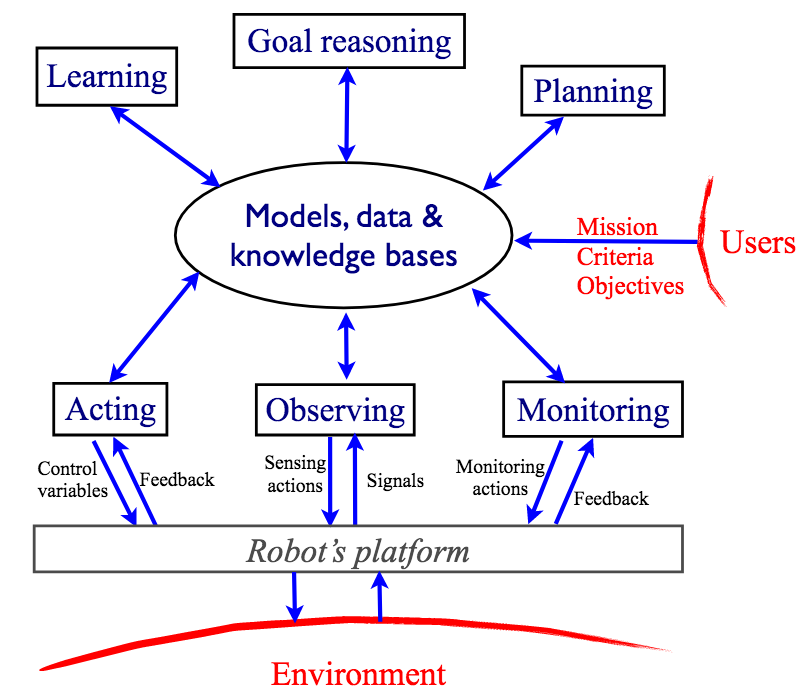
\includegraphics[scale=0.50]{figures/deliberationfunctions}
	\caption{Schematic view of deliberation functions \cite{ingrand2017deliberation}}
	\label{fig:deliberationfunctions}
\end{figure}

The framework that we propose with this project allows users without any programming knowledge to teach a robot a goal-oriented behaviour. 
Unlike current PbD implementations, which teach the robot an action sequence to achieve a goal, we want to equip the robot with all actions required to generate the action sequence autonomously using automated planning techniques. The user needs to construct a planning domain, consisting of all actions that the user taught the robot by demonstration.
 Using this knowledge base, the user can define a planning problem, for which the robot will generate a plan.
 PbD implementations using Hidden Markov Models recognise examples from training sets and use probabilities to assign an action.
 This requires training sets that are large enough to cover a wide range of possible world states.
 With our goal-oriented approach, the robot can solve an infinite number of goals, by using a limited set of actions.
 Figure \ref{fig:framework} shows the layout of our proposed framework (user activities are shown in blue and robot activities are shown in red).
 

  \begin{figure}[!h]
    \centering
    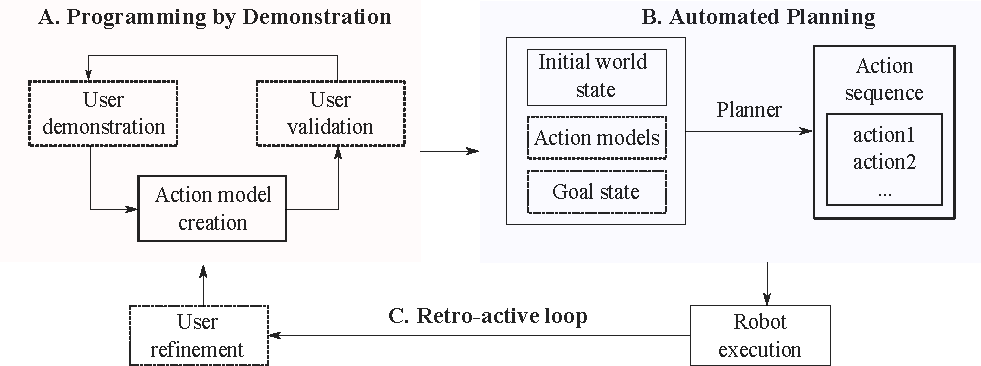
\includegraphics[width=\linewidth]{figures/framework}
    \caption{Framework for Robot Programming by Demonstration}
    \label{fig:framework}
  \end{figure}

\section{Creation of the Knowledge Base}
The user (in blue) interacts with the robot (in red) using a graphical interface.
The user has to create the planning domain, as specified in \sect{subsec:Planning domain description}, by defining the requirements, object types and predicates, i.e. conditions that can be included in the action definition.
The graphical interface should present the PDDL definitions in English sentences for the user.
Note that the object type definition at this stage is only at a syntactical level.
The instantiation of the locations and objects only occurs in the problem definition.
This leaves the user with the creation of the action models.

The actions will be created sequentially by iteratively providing demonstrations of the each individual action.
The robot extracts the relevant information from the demonstration using its sensors and builds a model of the learned skill.
By observing the changes in the state of the world, the robot suggests preconditions and effects, selected from the domain description, to be associated with the taught action.
After each demonstration, the user is presented with options to reproduce the learned skill or to modify the observed conditions.
The user either validates the learned action or provides another demonstration to refine it.
 

The action can be learned by generalising over a set of trajectories and by using statistical learning techniques, to deal with uncertainty contained in multiple motion demonstrations (\cite{ude1993trajectory}).
Once the user is confident about the created action model and its associated conditions, they can save it to the knowledge base.
 This process is repeated for all action models that are required to build the knowledge base for the complex task.
 The action models are automatically translated into PDDL, allowing the creation of a PDDL domain, without the requirement for any programming knowledge.

\section{Task Execution}
The created knowledge base is internally connected with a planner.
 The user needs to create a planning problem, as specified in \sect{subsec:PPDescription}, by listing all objects of the planning problem.
 To associate the PDDL objects with the physical objects in the real world, the user needs to assign features to each object in the planning problem, to allow their easy recognition.
 For instance, the robot can learn to recognise objects by their colour or shape, and locations can be saved using their end effector coordinates.

Instead of defining the initial state, the robot should recognise it using its sensors, allowing the user to verify the robot's learned object recognition.
 Once the planning problem has been defined, the robot can generate a plan.
 The action sequence will then be executed by the robot in order to achieve the goal state.
 If the user changes the goal, a new plan will be generated accordingly.
This removes the intermediate step of having to define an action sequence manually every time the goal changes.
 
If the proposed solution is not optimal, the user can modify them or refine the action models.
 Missing predicates in the action definition can lead to suboptimal solutions.
 The generation of an action sequence provides the user with the opportunity to test the soundness of their created action models.\\

\noindent In summary, our proposed framework links techniques from the two disciplines Programming by Demonstration and Automated Planning to create a means for the non-expert user to teach a robot a goal-oriented behaviour.
 The user's steps can be summarised as follows:

\begin{enumerate}
\item Define the requirements, types and predicates for the domain description.
\item For all actions:
\begin{enumerate}
\item Record an action demonstration for the robot learner.
\item Verify the derived policy and validate the proposed preconditions and effects.
\item Optionally provide additional demonstrations to refine action.
\end{enumerate}
\item Define a planning problem using the created domain, including a goal state.
\item \textit{The robot recognises the initial state and generates a plan.}
\item Verify that the action sequence of the plan is correct.
\item Optionally refine the created action models.
\end{enumerate}


%\chapter{Experimentation and Evaluation}\label{chap:Evaluation}
%\minitoc% Creating an actual minitoc
\section{System Evaluation}
\label{sec:syseval}
We evaluate our system's generalisability on six benchmark tasks (Table \ref{table:task-list}) and show how taught primitive actions can be reused for complex tasks.
The tasks involved manipulating different object types on four marked positions with both claw and suction grippers.
We take the Blocksworld domain \cite{slaney2001blocks} for building and rebuilding stacked objects (Tasks 1-4) and an elaborate version of the Tower of Hanoi problem with different object types to build a `house' (Tasks 5\&6).
Instead of disks, we decided to use different object types (ROOF, CUBE, BASE), where BASE corresponds to the largest disk, followed by CUBE and BASE.
The rules for stacking different objects still apply (\eg BASE cannot be stacked on top of ROOF or CUBE).
However, to demonstrate the generalisation of actions to diverse tasks, additional constraints are added as objects cannot be all manipulated in the same way.
The order of the tasks was given with increasing complexity, requiring the user to modify existing actions or teach new actions from scratch.
% to show reusability of more and more complex tasks we use the Tower of Hanoi problem with different number of disks, to show its applicability in real-world, we take an assembly task.
% The most common tasks for industrial robots are assembly, packaging, and material handling (such as polishing etc.) \footnote{https://blog.robotiq.com/the-3-most-common-tasks-delegated-to-robots-in-manufacturing}.
%Picking, Packing and Palletizing – Most products are handled multiple times prior to final shipping. Robotic picking and packaging increases speed and accuracy along with lowering production costs \footnote{https://www.jabil.com/insights/blog-main/ten-popular-industrial-robot-applications.html}
% Assembly and packaging tasks require prior planning in order to complete a task efficiently.
%Thus, we take an assembly task to build a ..and a packaging task with.


\begin{table}[t]
\begin{center}
\caption{Benchmark tasks for the system evaluation. Three different pick-and-place actions were programmed.}
\label{table:task-list}
%\begin{center}
\begin{tabular}{clll}
\# & Task Goal & Pick-and-place action\\ \hline
1 & Build tower with 3 CUBES & claw from top \\
2 & Build tower with 4 CUBES & claw from top \\
3 & Rebuild Task 2 on a different position & claw from top \\
4 & Build tower and move (w/o disassembly) & claw from top \& side \\
5 & Build house with BASE, CUBE, ROOF & claw \& suction from top \\
6 & Rebuild Task 5 on a different position & claw \& suction from top \\
% 5 & Assembly & P\&p with turning/orienting \\
% 6 & Packaging & P\&p with pushing to save space \\
\end{tabular}
\end{center}
\end{table}

\subsection{Protocol}
The tasks were programmed by one of the authors, with the most efficient teaching strategy of minimising the number of actions created and generalising them by changing the action properties (as described in \sect{sec:generalisation}).
Depending on the given task and involved objects, the experimenter decided what manipulation action needed to be taught.
Only one planning problem was created and reused for all tasks by redetecting the objects in the initial state and changing the goal state.
When the generated plan was incorrect, the debug menu on the GUI was used to determine the changes to be made to generalise the actions.
A task was considered completed when the generated plan was correct and the robot successfully executed it in real-time.
As the mental model saved the latest object positions after an action execution, Tasks 3 and 6 were continued from the preceding tasks and did not require redetecting the initial states. 
%reusing the problem with the latest saved mental model allowed them to overcome the limitation to detect stacked objects.

\begin{figure*}[h]
	\centering
	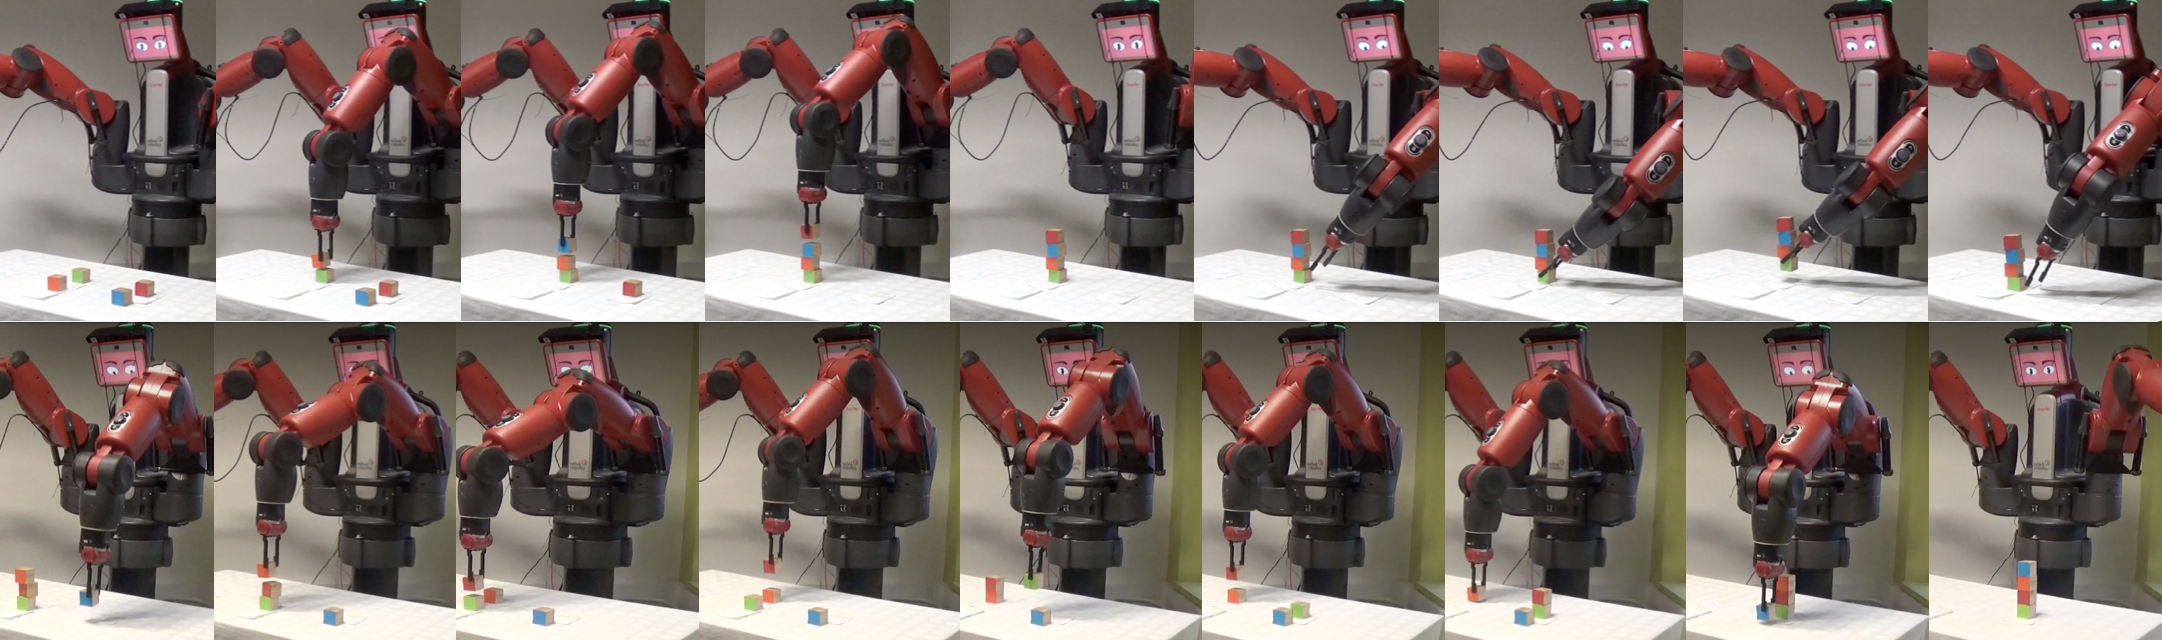
\includegraphics[width=\linewidth]{figures/filmstrip.png}
	\caption{Snapshots from the executions of the system evaluation (Tasks 3\&4) showing a claw grip from top and side.}
	\label{fig:filmstrip}
\end{figure*}

\subsection{Results}
We programmed three manipulation actions for the six benchmark tasks, which involved demonstrating pick-and-place actions with claw and suction grippers from the \textit{top} and from the \textit{side}.
Actions were generalised by changing parameter types (\eg from CUBE or POSITION to ELEMENT) or adding preconditions or effects which were not inferred automatically.
For pick-and-place actions from the top, `obj is clear' was added as a precondition (Task 1-3), while it was not included when picking an object from the side to allow moving a pile of objects (Task 4).
For actions involving the claw gripper, the precondition `obj is thin' was added so that the robot would only use it on ROOF and CUBE objects, similarly `is flat' for the suction gripper (Task 5\&6).
The `is stackable' condition was used for the Tower of Hanoi as an equivalent to the rule `larger objects cannot be placed on top of smaller ones'.
The robot was able to generate plans for all tasks and executed them in real time at least twice (\fig{fig:filmstrip}).\footnote{A subset of the task executions can be seen in the attached video}
Note that the taught primitive actions can be reused for a diverse range of problems beyond the six benchmark tasks.
This evaluation shows the generalisability of our system, allowing us to teach primitive actions by demonstration and reuse them with a task planner to solve more complex problems.


\section{User Evaluation}
\label{sec:quanteval}
The second part of the evaluation was conducted using the THEDRE (Traceable Human Experiment Design Research) method (\cite{mandran2018traceable,mandran2017thedre}) which aims to evaluate computer systems in a research context by integrating a user-centered approach.
It is based on continuous improvement and takes a pragmatic constructivist approach (\cite{avenier2015finding}), allowing it to further develop the system as well as the scientific knowledge from the experimental ground.
To that end, it offered us the possibility to mix qualitative and quantitative approaches in order to gather as much data as possible to evaluate and improve our system. 

User experiments aimed to evaluate our approach implemented on a Baxter robot with real end-users.
However, we were also interested in the user's programming strategy of using the system.
Thus, we split participants into two control groups, with and without condition inference (\sect{sec:inference}) and observe user strategies for completing the tasks.
%if they had the tendency of `blindly trusting the system'.
% \subsection{Hypotheses}
We set the following hypotheses for our experiments:
\begin{enumerate}
    \item[H1] Action creation: users can teach new low- and high-level actions by demonstration
    \item[H2] Problem solving: users can solve new problems by defining the goal states and executing the plan on Baxter
    \item[H3] Autonomous system navigation: users understand the system and can navigate and troubleshoot on their own
    \item[H4] Condition inference evaluation - Group 1 vs 2: users without automatic condition inference will understand the system better
    \item[H5] Pre-test questionnaire: users that perform better in the pre-test questionnaire can learn to use the system faster
\end{enumerate}

\subsection{Set up}
The experiments were conducted with a Baxter robot with two grippers (suction and claw) and mounted with a Kinect Xbox 360 camera. 
A table with 4 marked positions was placed in front of the robot with different objects to be manipulated by the robot during the experiment (\fig{fig:dispositif}).
Participants had access to a computer with a mouse and a keyboard to program the robot via the graphical interface.

\subsection{Participants}
The study was conducted with 21 participants (10M, 11F) in the range of 18-39 years (M=24.67, SD=6.1).
We recruited participants with different educational background and programming levels: 
6 `CS' (either completed a degree in computer science or were currently pursuing one),
7 `non-CS' (have previously taken a programming course before), 
and 8 `no experience' (only had experience with office productivity software).
Furthermore, 3 participants (in `CS') have programmed a robot before, out of which 1 had intermediate experience with symbolic planning languages while the remaining participants had no experience in either.
One participant in the category `non-CS' failed to complete the majority of tasks and was excluded from the result evaluation.
The two control groups included equal number of participants in all three categories.

\subsection{Protocol}
Users were first given a brief introduction to task planning concepts, the Baxter robot and the experimental set up.
They were then asked to complete a pre-study questionnaire to capture the participant's profile and their understanding of the presented concepts.
Users were given 8 tasks to complete, where the first two were practice tasks to introduce them to the system (Table \ref{table:userstudytasks}). 
The tasks were designed to address different aspects to familiarise them with the system:
create new actions (Task 6), modify parameter types (Tasks 4\&7), modify action conditions (Tasks 3,5,8).
For each task they needed to create a new problem, define the goal states, and launch the planner to generate an action sequence.
When the generated plan was correct, they were executed on the robot.
Otherwise, the user had to modify the existing input until the plan was correctly generated.
Tasks 6-8 were similar to the previous tasks (1-5) but use both robot grippers.

\begin{table}[h]
	\centering
	\caption{Benchmark tasks for the user study where the first two tasks were used to introduce participants to the system.}
	\label{table:userstudytasks}
	\begin{center}
		\begin{tabular}{ll}
			\# Task description & Main solution \\ \hline
			(1) move a BASE object & create new action (+demo) \\
			(2) move a BASE object to any position & create new problem \\
			3 swap two BASE objects & add condition (`is clear') \\
			4 stack a CUBE on a BASE & modify types\\
			5 do not stack a CUBE on a ROOF & add condition (`is stackable')\\
			6 move a ROOF object & create new action (+demo) \\
			7 stack a ROOF on a CUBE & modify types  \\
			8 build a house (BASE, CUBE, ROOF) & navigate autonomously \\ \hline
		\end{tabular}
	\end{center}
\end{table}

\subsection{Metrics}
We captured the following data during the experiments:
\begin{enumerate}
    \item \textbf{Qualitative data:} video recording of the experiment, observations during the experimental protocol.
    \item \textbf{Quantitative data:} task duration and UI activity log, pre-study questionnaire, post-study survey.
\end{enumerate}

The pre-study questionnaire included 7 questions related to their understanding of the concepts presented at the start of the experiment, \eg syntax (`If move(CUBE) describes a move action, tick all statements that are true.'), logical reasoning 
(`Which two conditions can never be true at the same time?'), and other concepts (`Tick all predicates that are required as preconditions for the given action').
The questions were multiple choice and each question was normalised to count at most 1 point if answered correctly.
The highest achievable score was 7.
%Answers that were selected incorrectly were penalised with half a point
%to discriminate users who selected unnecessary options

In the post-study survey we used the System Usability Scale (SUS) (\cite{brooke1996sus}) where participants had to give a rating on a 5-Point Likert scale ranging from `Strongly agree' to `Strongly disagree'.
It enabled us to measure the perceived usability of the system with a small sample of users (\cite{tullis2004comparison}).
As a benchmark, we compare overall responses to our previous user study in \sect{sec:Exp2}, where users were simulated a robot programming experience using the Wizard-of-Oz technique.
Finally, participants were asked which aspects they found most useful, most difficult, and which they liked the best and the least.


% We compared the following data:
% \begin{itemize}
%     \item Participant profile (background, experience with programming/robots)
%     \item Pre-study questions on basic task planning concepts (i.e. predicate logic)
%     \item Post-study questionnaire on usability of the system
%     \item Notes during the experiment on user’s attempts/difficulties/etc.
%     \item UI activity log: timestamps of any button clicks
%     \item Number of tasks completed
%     \item Duration per completed task
% \end{itemize}

\subsection{Results}
20 participants completed all tasks, while one `non-CS' user failed to complete the majority of tasks and did not seem to understand the presented concepts.
This participant was excluded in the presented results.

\subsubsection{User performance (H1-H3)} 
%After the initial introduction to the system (Tasks 1\&2), all participants stated that they understood the difference between \textit{Actions} and \textit{Problems}.
Users took an average of 41.2 minutes (STD=9.08) to complete the main tasks (3-8).
`non-CS' users completed the tasks the fastest (AVG=36.6, STD=7.46), followed by users with no programming experience (AVG=43.6, STD=5.37).
`CS' users took on average longer (AVG=43.8, STD=14.13) as they were often interested in testing the system's functionalities with different inputs.

% \todo{check end time of last task is consistent}
%Task 1: Group 1: 7/10 participants did not modify the conditions and confirmed them directly. 
%
% \textbf{Task 2} (move BASE to any other position):
% 4 participants tried to set the goal as `obj is not on posM'. 
% This did not produce a plan as the action conditions were missing the right predicate.
Users initially had problems with different concepts that were presented at the start of the study, in particular they confused action parameters, preconditions and goal states.
For example, in Task 3, 6 (or 30\%) users tried to add intermediate action steps to achieve the goal state, instead of simply letting the planner generate the solution.
In Task 4, 14 (or 70\%) wanted to create a new action instead of generalising the existing one by changing the parameter types.
However, by Task 6, all users were able to use the system autonomously to create new actions and problems and navigated the system with little to no guidance.
%
% \textbf{Task 3} (generate plan for swapping two objects):
% To solve Task 3 (generate plan for swapping two objects), at least 6 participants tried to add intermediate action steps that should achieve goal state, instead of simply stating the predicates that described the goal state and letting the planner generate a solution.
% 4 users did not verify the plan and executed it directly, causing the robot to execute a wrong plan.
%
%\textbf{Understanding the predicates: }
% \textbf{Task 4} (stack CUBE on BASE):
% 5 participants tried to add `CUBE is stackable on BASE' as a goal state.
% Only 2 participants thought about changing the action parameter type directly.
% The other 20 participants were given a subproblem where the CUBE had to be placed on a position instead of the BASE.
% The majority of users (14 or 70\%) wanted to create a new action instead of generalising the existing one or wanted to include two objects in the action definition.
% This is understandable as the users were not familiar with the system.
% Only 4 participants changed the POSITION to ELEMENT while the remaining 17 needed guidance.
%
% \textbf{Task 5} (do not stack cube on roof):
% 8 participants who have modified the action preconditions in Task 1 have already added this condition. 
% 3 required no guidance to add this condition.
% The remaining 10 required guidance, some tried to add conditions related to the ROOF object type (such as `do not stack if it is a ROOF') rather than the general property of stacking it only if the target is flat or stackable.
%
% \textbf{Task 6} (create new move ROOF action):
% The majority of participants did not encounter any problems when creating the new action and required little to no guidance.
% 2 participants encountered problems with the manipulation of Baxter's arm during the kinesthetic demonstration.
% 4 participants forgot to add conditions after the demonstration step.
% Only 2 participants changed the types of the new roof action to generalised types as seen before.
% 7 participants added preconditions that were needed in the previous tasks (is clear, is stackable), while the remaining 14 only kept the minimum set of conditions.
%
% \textbf{Task 7} (stack ROOF on CUBE):
% All participants changed the parameter type to allow stacking on any element. 
% When the generated plan tried to use the wrong gripper, a new precondition (`obj is flat') needed to be added:
% 8 participants had already added this in the previous tasks, while 4 needed guidance to add this condition. 
% \textbf{Task 8} (build a house):
% Missing precondition `obj is clear':
% 6 participants had already added this condition previously, 3 added them without guidance, 4 with guidance, and the remaining failed to add this condition.
%Out of the 6 benchmark tasks, X completed all tasks.
By the end of the experiment, users programmed two manipulation actions (one for each gripper).
The generated PDDL code for the planning domain can be found in the attached material.


% \begin{figure}[tb]%
%   \centering
%   \begin{subfigure}[h]{0.24\textwidth}%
%     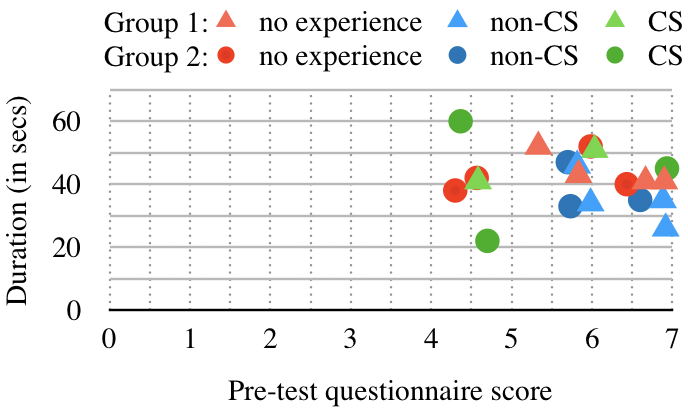
\includegraphics[width=\textwidth]{figures/quan-pretest-results.png}%
%     \caption{Pre-test vs Task duration}\label{fig:pretestvstask}%
%   \end{subfigure}~~%
%   \begin{subfigure}[h]{0.24\textwidth}%
%     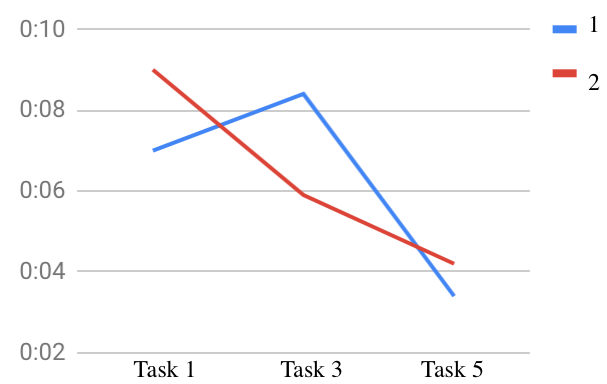
\includegraphics[width=\textwidth]{figures/quan-groups-duration.png}%
%     \caption{Task duration per group}\label{fig:taskvsgroup}%  
%   \end{subfigure}
%   \caption{}
%   \label{fig:task-duration}%
% \end{figure}%

% \begin{figure}[tp]
%   \subfigure[Pre-test vs Task duration]{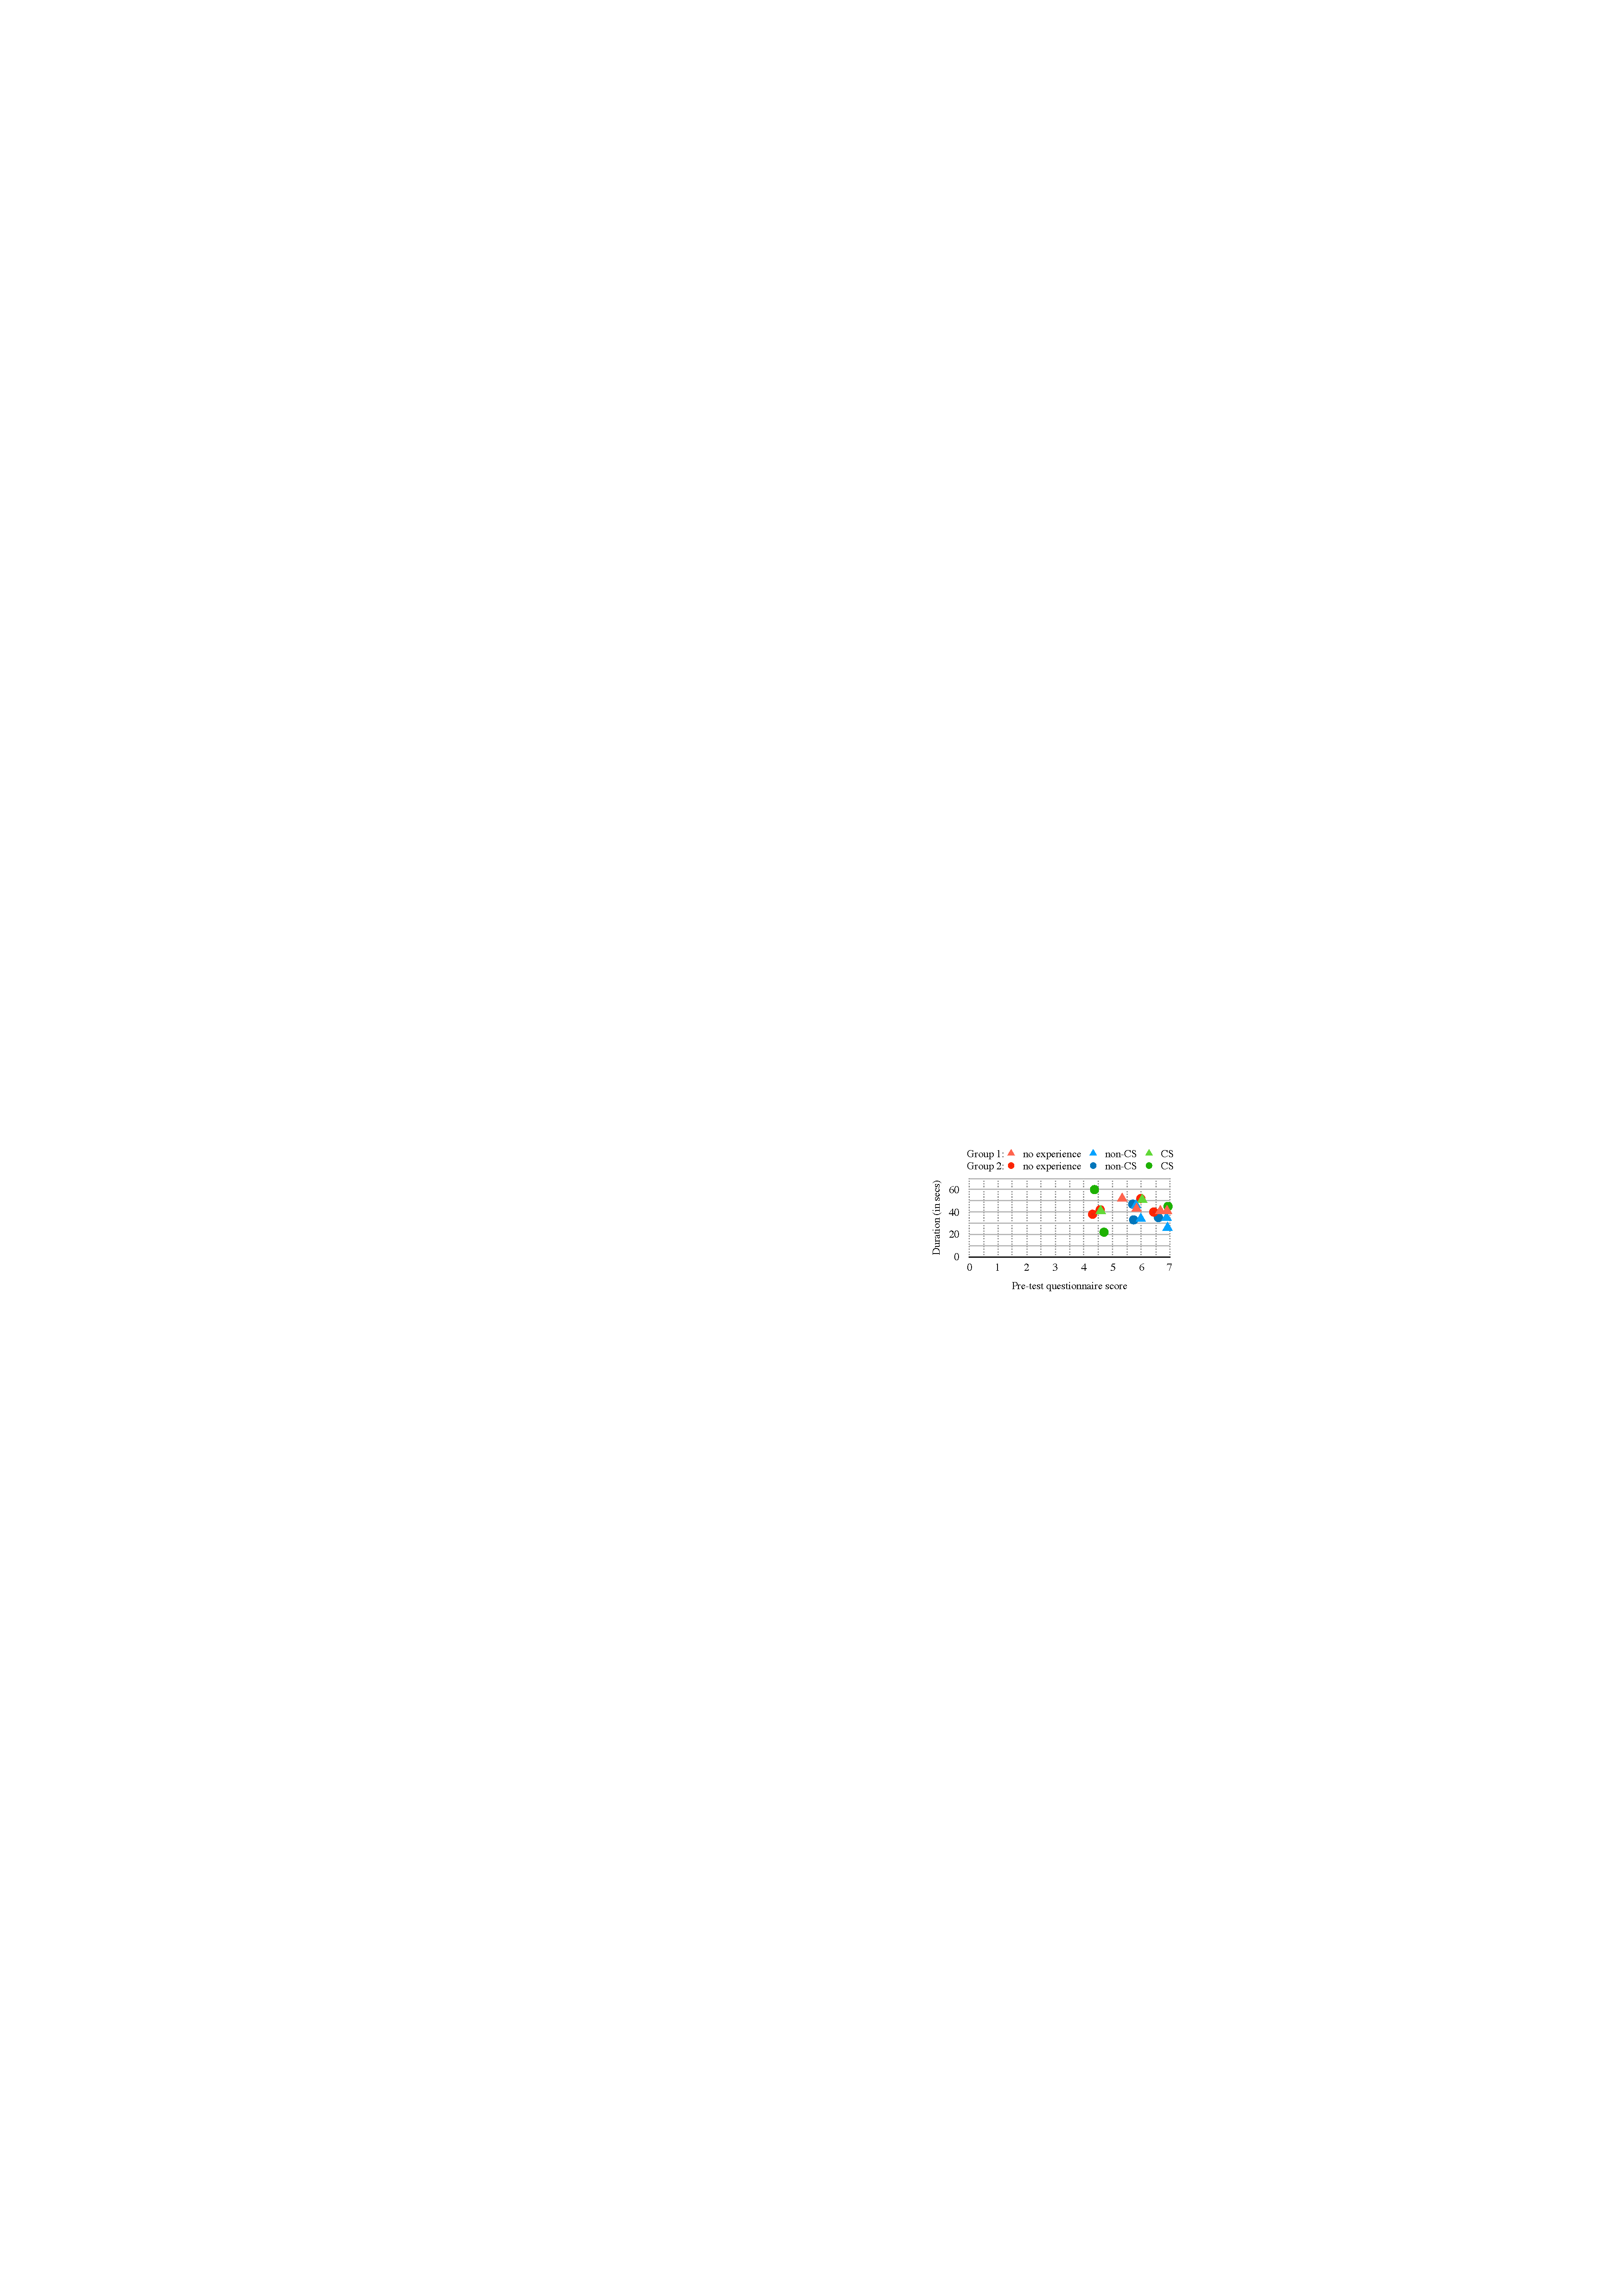
\includegraphics[width=0.48\linewidth]{figures/quan-pretest-results.pdf}}
% \label{fig:pretestvstask}\quad
%   \subfigure[Task duration per group]{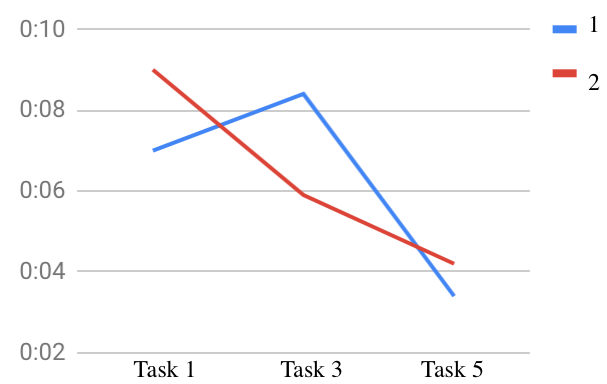
\includegraphics[width=0.48\linewidth]{figures/quan-groups-duration.png}}
% \label{fig:taskvsgroup}
% \end{figure}

\subsubsection{Condition inference (H4)} 
To evaluate user programming strategies, the condition inference (CI) (see \sect{sec:inference}) in our study only generated a minimal set of predicates, which did not cover predicates needed for later tasks.
We noticed a discrepancy in the programming strateg between the two control groups (Group 1 with CI vs. Group 2 without CI).
As participants in Group 2 had to add action conditions manually, they considered all predicates they deemed necessary for the action and therefore added additional ones that were required for later tasks.
On the other hand, we observed that Group 1 had the tendency to leave the inferred conditions unmodified without adding conditions that were missing.
%7/10 users in Group 1 did not modify the inferred conditions and did not put much thought potentially missing conditions.
Thus, Group 2 took on average longer to complete tasks where a new action had to be created (Tasks 1\&6), but was faster than Group 1 for subsequent tasks, where conditions had to be modified (Tasks 3,5,7).
Overall both groups had similar completion times for all tasks (Group 1: AVG=41, STD=7.89 and Group 2: AVG=41.4, STD=10.56).

\subsubsection{Task duration vs Pre-test questionnaire (H5)} 
As expected, participants who demonstrated a better understanding of the introduced concepts in the pre-test questionnaire completed the main tasks (Tasks 3-8) faster on average (\fig{fig:pretestvstask}).
Users scored between 4.3-6.93 out of 7 points (AVG=5.8, SD=0.91), with task completion times between 22-60 minutes (AVG=41.2, SD=9.07).
`non-CS' users scored above average points (AVG=6.23, STD=0.55) and completed the fastest (AVG=36.6, STD=7.46).
As an outlier we observed that the fastest participant scored only 4.7, but easily learned how to use the system and completed the tasks in 22 minutes.
%the participant that took the longest (60min) scored 4.37.
Even though Group 1 performed slightly better in the pre-test (AVG=7.5, STD=1.35) than Group 2 (AVG=6.4, STD=2.01), both completion times were on average similar (41min).

\begin{figure}[h]%
	\centering
	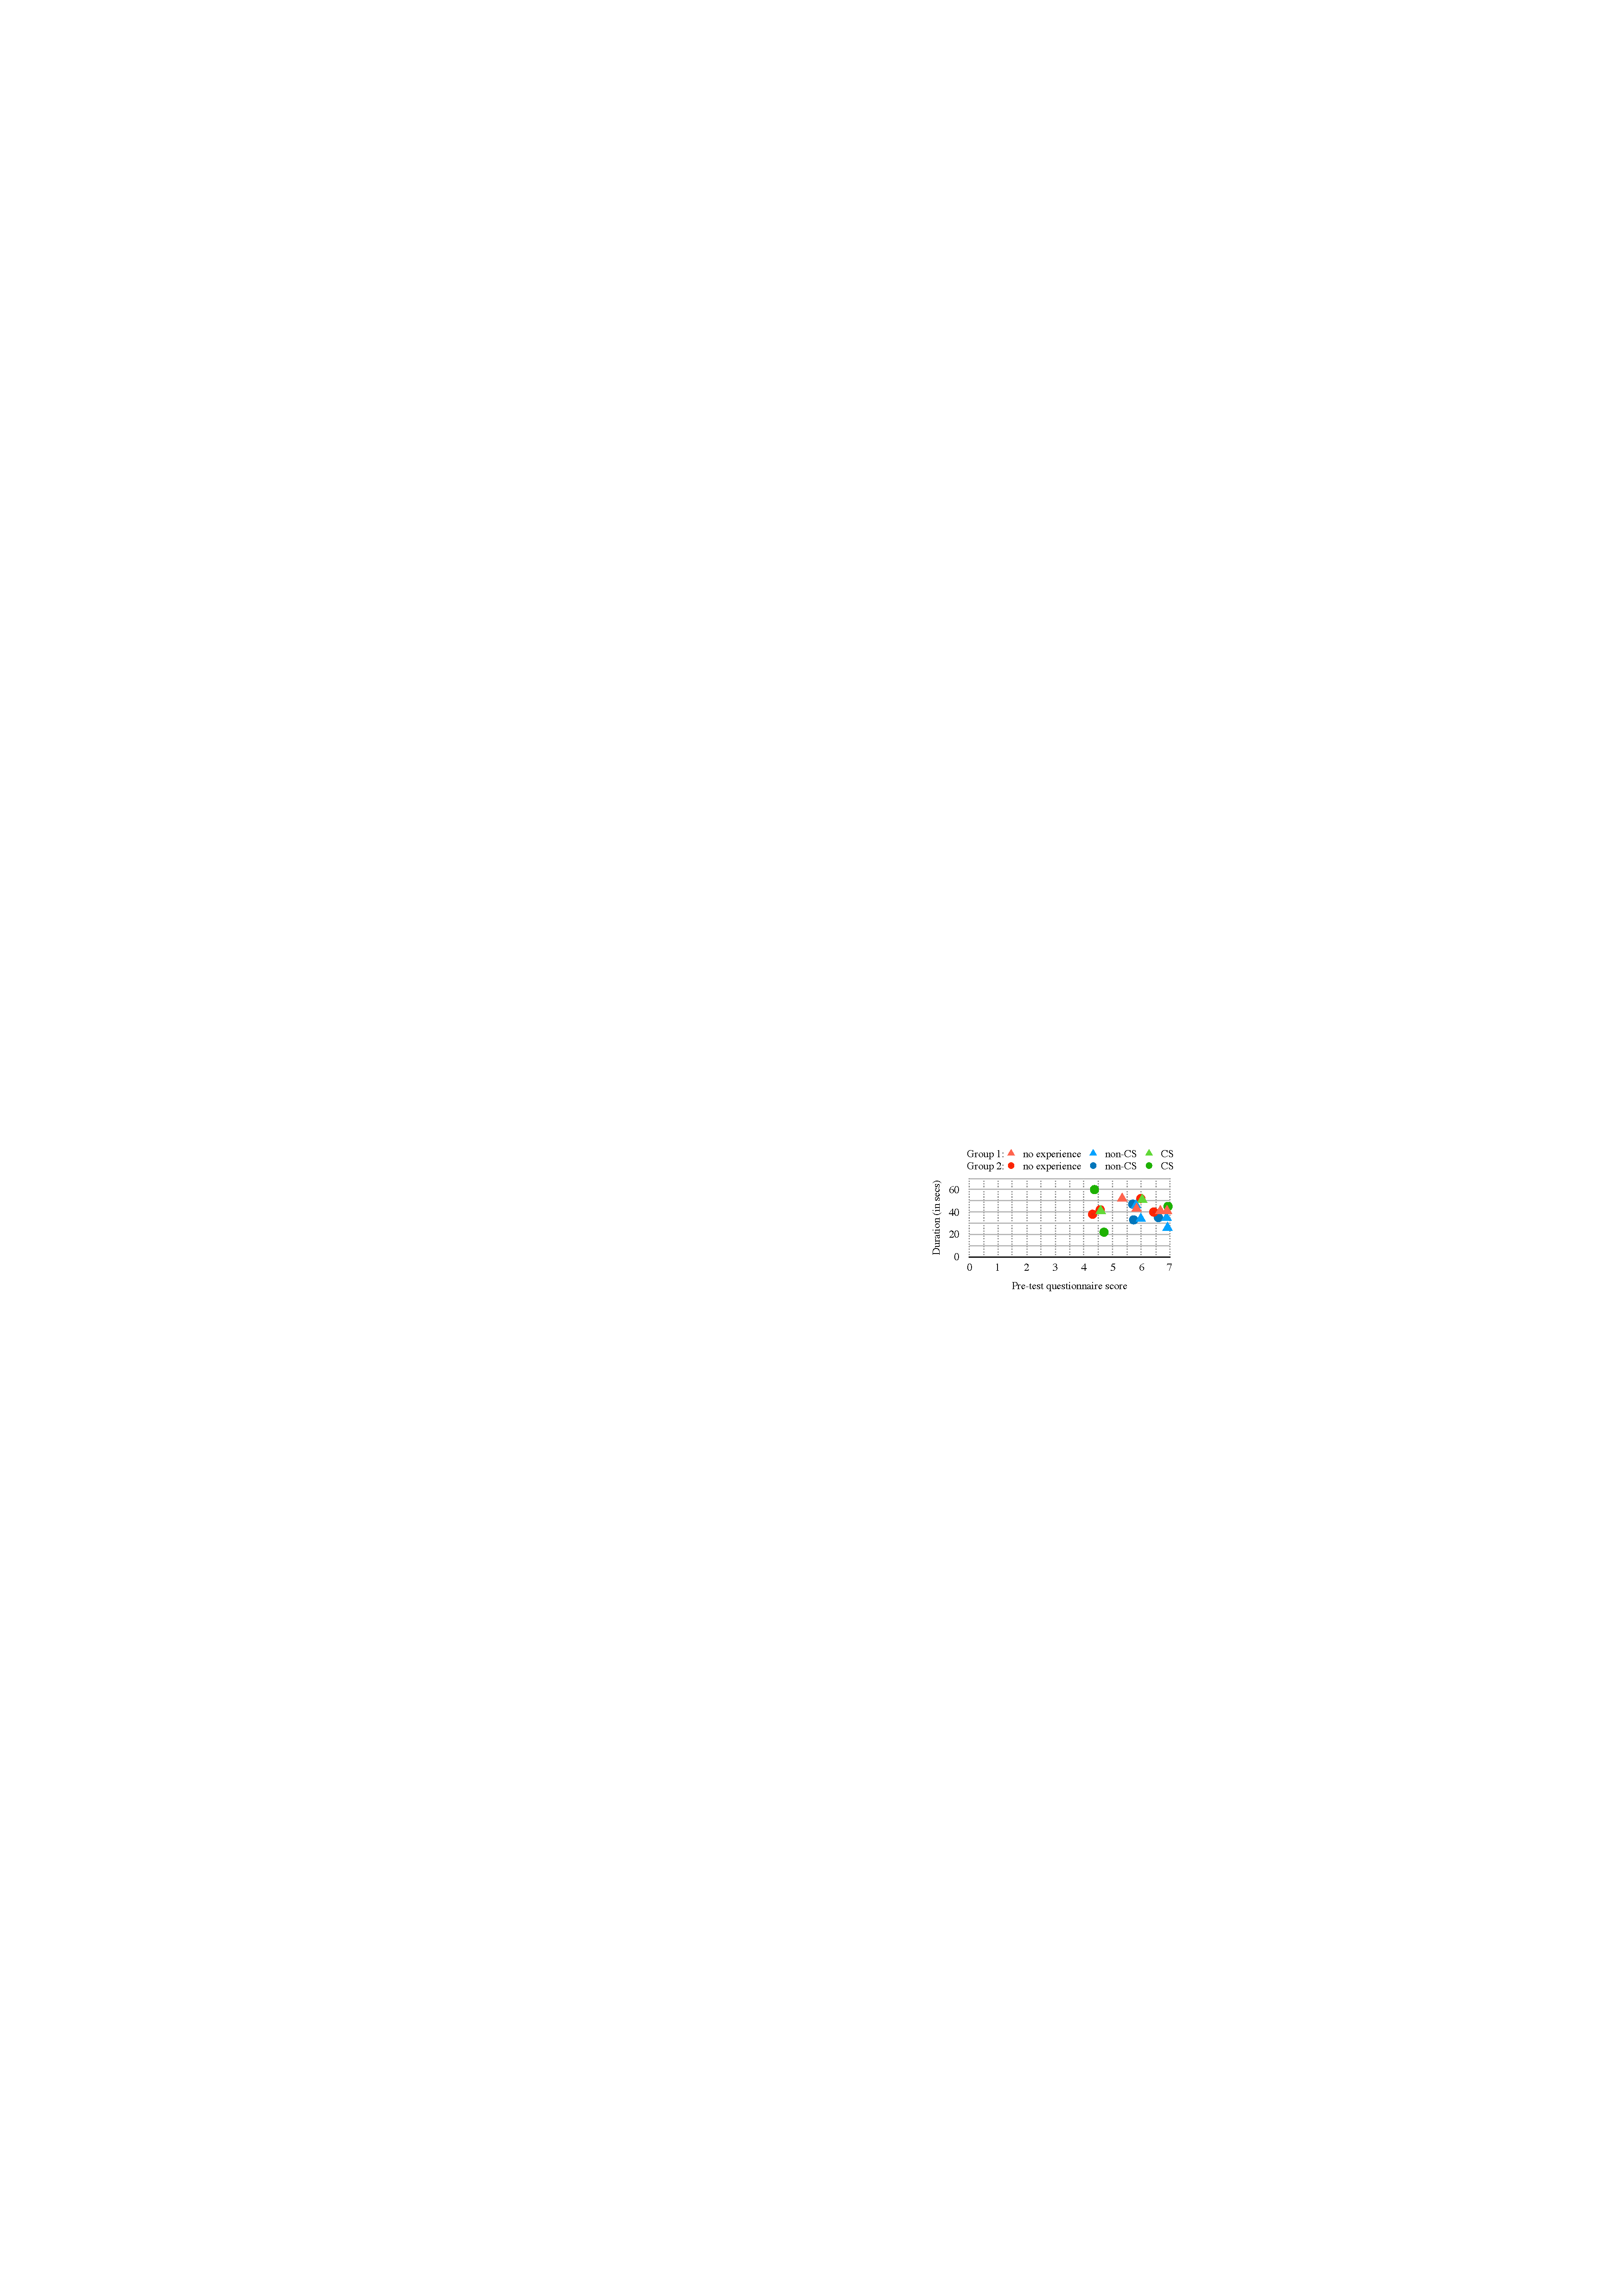
\includegraphics[width=0.5\columnwidth]{figures/quan-pretest-results.pdf}%
	\caption{Participants who did better in the pre-test questionnaire completed the main tasks faster, with `non-CS' users scoring the highest and being the fastest on average.}\label{fig:pretestvstask}%
\end{figure}%
%In Task 3: as all the users in Group 2 had added the missing condition (`posB is clear') in Task 1, a correct action sequence was generated directly.
%In Group 1 8/10 had not added this condition and needed guidance to resolve this issue, with 3 participants trying to modify the problem definition instead of the action, 1 trying to add a new action for `clearing a position', and 1 failing to figure out the right condition to add.


% \begin{table}[h]
% \centering
% \caption{TO DO: User performance with (Group 1) and without condition inference (Group 2) where Tasks 1 and 2 were training.}
% \label{table:performance}
% \begin{center}
% \begin{tabular}{ccc}
% Task & Group 1 & Group 2 \\ \hline
%  & Action/Problem & Action/Problem \\
% (1) & 0:30 () & 0:40 \\
% (2) & 0:30 & 0:40 \\ \hline
% 3 & 0:30 & 0:40 \\
% 4 & 0:30 & 0:40 \\
% 5 & 0:30 & 0:40 \\
% \hline
% %6 & (3,3,1) off-grid & Pick, place, push left\&front & Tin cans \\
% %7 & (3,3,1) off-grid & Pick, place, push left\&front& Soda cans \\
% %8 & (2,3,1) interleaving & Pick and place from top & Candy bags \\ 
% Total & 0:30 & 0:40 \\ \hline
% Pre-Test Score & 8/10 & 7/10 \\ 

% \end{tabular}
% \end{center}
% \end{table}

\subsubsection{System usability and learnability} 
There are several ways to interpret the System Usability Scale (SUS) scores (\cite{brooke2013sus}) obtained from the post-study survey. 
Using \citet{bangor2008suseval} categories, 14 (70\%) users ranked iRoPro as `acceptable', 6 (30\%) rated it `marginally acceptable', and no one ranked it `not acceptable'.
Correlating this with the Net Promoter Score\footnote{https://measuringu.com/nps-sus/}, this corresponds to 10 (50\%) participants being `promoters' (most likely to recommend the system), 5 (25\%) `passive', and 5 (25\%) `detractors' (likely to discourage).
Overall, iRoPro was rated with a good system usability which has been shown to be correlated with its learnability (\cite{borsci2009dimensionality,sauro2011practical}).

\subsubsection{User experience} 
%We asked users the same questions as in our previous work \textit{[Anonymous]} where we used the Wizard-of-Oz technique to conduct a qualitative evaluation of a potential system.
% similar with mainly positive responses in both studies .
Comparing the responses to the user study conducted in \sect{sec:Exp2}, where the Wizard-of-Oz technique was used to simulate the robot programming process, the main difference was regarding difficulties encountered during the experiment.
While in \sect{sec:Exp2} we had 11 (or 100\%) agree that they encountered no difficulties, only 7 (or 35\%) of our users in this study stated the same (\fig{fig:exp1vsexp2-results}).
However, all of our users claimed to have a good understanding of the action representation and how the robot learned new actions from the demonstration, while in the previous study, an average of 2 (18\%) disagreed.
Both differences can be explained by the fact that in our latest study, users had to use an end-to-end system to program the robot, while we previously simulated the system functionalities using the Wizard-of-Oz technique.
Even though our users encountered more difficulties, they got a better understanding of the functionalities due to getting hands-on experience.
This also correlates with negative responses in our survey to the question if `no programming experience was required' where 13/20 (65\%) agreed and 4 disagreed.
%3 out of the 4 who disagreed had at least taken a programming course before.
Overall, our user study with iRoPro received positive responses similar to our previous study.

Users stated the most useful feature as `generate solutions to defined goals automatically' (9 or 45\%), followed by `robot learns the action from my demonstration' (4 or 20\%) -- two main aspects of our approach.
A common feedback was that `it takes time to understand how the system works at the start'.
4 (20\%) stated that the most difficult part was `finding out why Baxter didn't solve a problem correctly', similarly 8 (40\%) stated difficulties related to `understanding predicates and defining conditions'. 
11 (55\%) disliked `assigning action conditions' the most, while the rest stated different aspects.
The most liked actions were `executing the generated plan' (8 or 40\%) and `demonstrating an action on Baxter' (7 or 35\%).
%Overall, users performed well in both control groups and gave positive feedback.

\begin{figure*}
	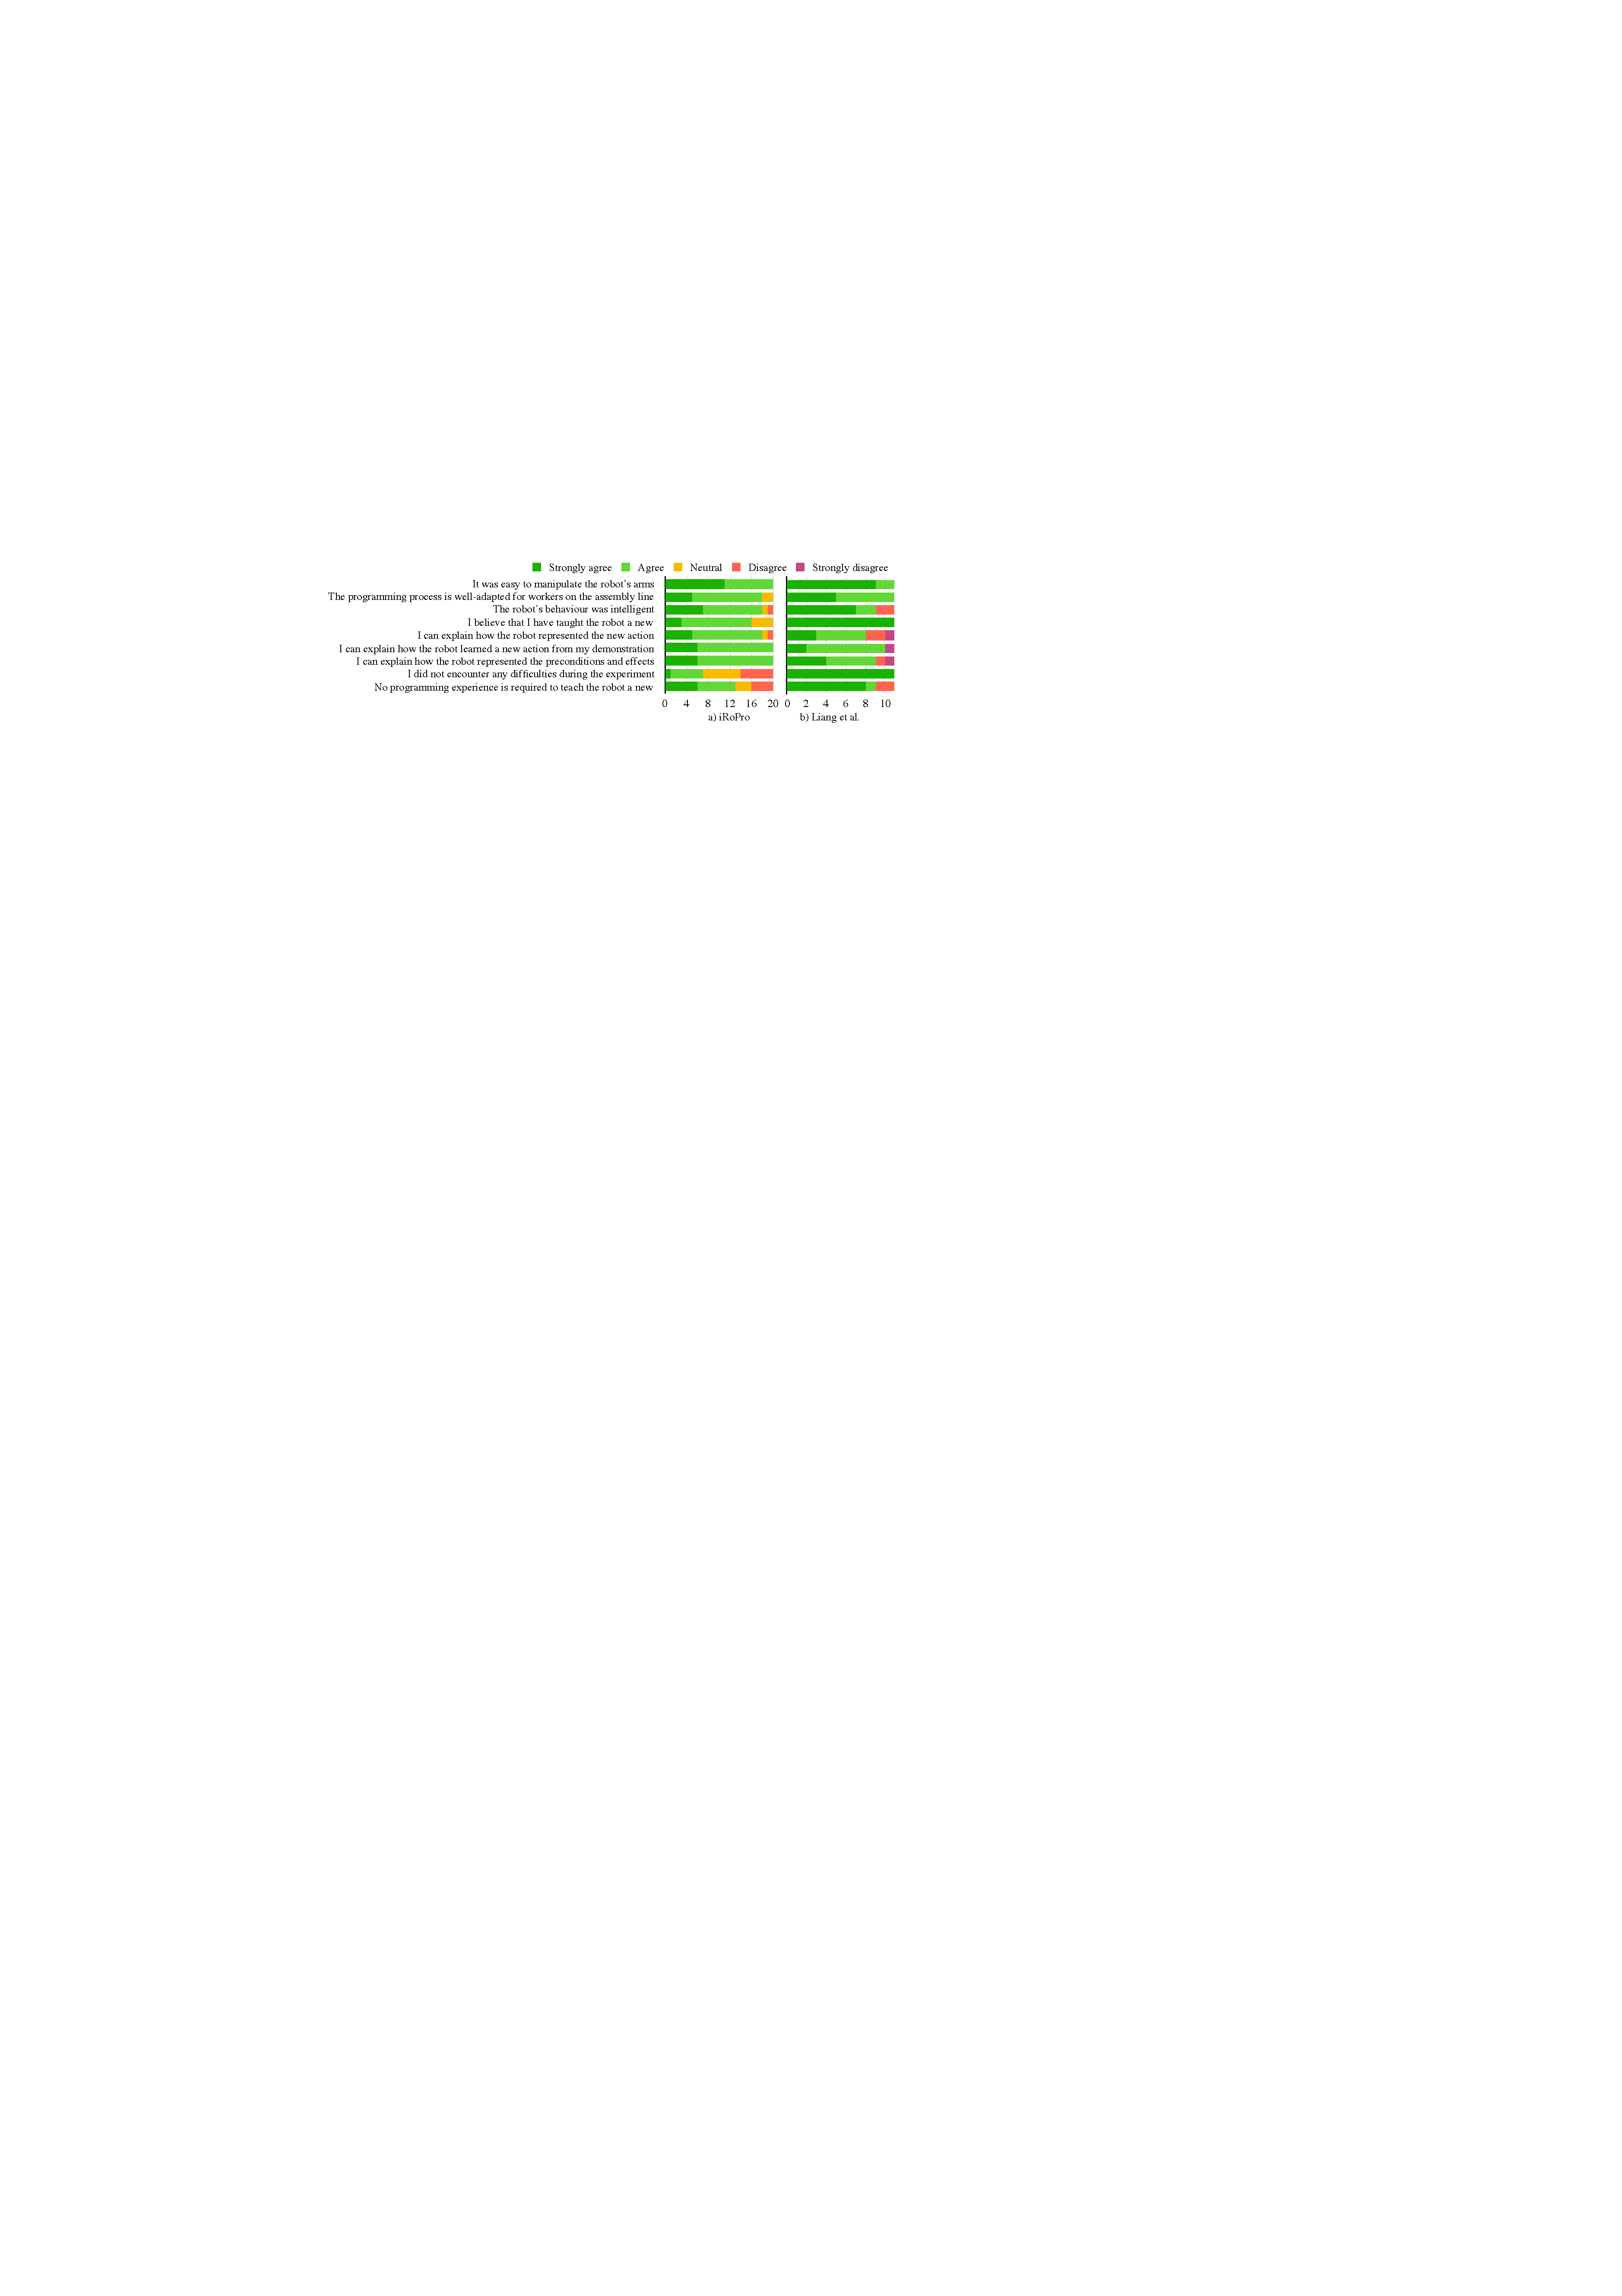
\includegraphics[width=0.98\linewidth]{figures/quan-exp1vsexp2-results.pdf}
	\caption{User responses from the post-study survey (N=20) comparing iRoPro to a similar user study (N=11) \cite{liang2017evaluation}}
	\label{fig:exp1vsexp2-results}
\end{figure*}
% \subsection{User strategies}
% As we have two control groups A (with condition inference) and B (without condition inference), we noticed two user strategies
% During the experiment, we noted the user's intended strategy to complete a task.

% \todo figure of people who tried the actions below:
% Teach new action
% Copy existing action
% Modify existing action

% \paragraph{User activity} 
% \todo {ignore some activity log at the end because of problems with executions} \\
% \todo {from Participant10 onwards, it keeps generating solutions for some reason}\\
% We logged the user activity on the interface at each button click to analyse the time spent on each task.

% The main activities 
% \todo {show graph of time spent at each option}
\section{Discussions}
\label{sec:discussion}
Both system and user evaluations demonstrated that iRoPro can be used to generalise primitive actions to a range of complex manipulation tasks and that it is easy to learn for users with or without programming experience.
In our system evaluation we could have programmed other actions, such as turning or pushing for packaging tasks.
As the purpose of our evaluation was to show the generalisability of primitive actions with the use of a task planner, we decided to stick to pick-and-place actions.
%Users particularly liked the PbD technique and found that
%`generating plans automatically' was the most useful feature 
In the following we discuss limitations and interesting extensions of our work:
\begin{enumerate}
	%\item No generalization from one item to another.
	\item Our object perception is limited as it does not detect objects that are too close together (\eg stacked objects).
	An improved perception system would allow the detection of initial states with stacked objects, automatically detecting goal states, or verifying action executions.
	%s mentioned in \sect{sec:implementation}, we partly the latter by using a mental model, where we first executed a stacking task to save the latest object positions, then reused the saved state for subsequent tasks.
	\item Due to the different grippers, we did not program actions that use both arms (\eg carrying a tray). A possible extension would be to include a better motion and task planning system in order to allow executing both arms simultaneously while avoiding self-collision.
	%As our robot was equipped with a suction and a claw gripper, the kinesthetic teaching of both arms could be difficult to program by a single user.
	\item We only included a minimal set of predicates (\sect{sec:highlevel}) that we deemed intuitive and useful for object manipulation tasks.
	It could be interesting to include and learn predicates to capture more complex domains such as object orientation (\cite{li2016learning}).
	%the use a mobile robot that can move between workstations.
	%\item A possible extension would be to incorporate probabilistic techniques to learn predicates or pre-train the robot on simulated scenarios to improve the condition inference.
\end{enumerate}


\section{Conclusion} 
\label{sec:conclusion}
In this chapter we presented iRoPro, an interactive Robot Programming system that allows simultaneous teaching of low- and high-level actions by demonstration.
The robot reuses the actions with a task planner to generate solutions to complex tasks that go beyond the demonstrated action.
The approach was implemented on a Baxter robot and we showed its generalisability on six benchmark tasks by teaching a minimal set of primitive actions that were reused for all tasks.
We further demonstrated its usability with a user study (N=21) where participants with diverse educational backgrounds and programming levels learned how to use the system in less than an hour.
Both user performance and feedback confirmed iRoPro's usability, with the majority ranking it as `acceptable' and half being promoters.
Overall, we demonstrated that our approach allows users with any programming level to efficiently teach robots new actions that can be reused for complex tasks.
Thus, we enable end-users to program robots from scratch, without writing code, therefore maximising the generalisability of taught actions with minimum programming effort.

\cleardoublepage
%\part{Conclusion}
\chapter{Conclusion and Future Work}\label{chap:Conclusion}
\minitoc% Creating an actual minitoc
\section{Contributions}
In this thesis we proposed a framework that uses PbD to teach a robot a goal-oriented problem-solving behaviour.
The framework combines solutions from PbD and Automated Planning, allowing non-expert users to teach a robot new actions together with their semantic meaning.
The user teaches the robot not only the action, but also its underlying meaning in terms of preconditions and effects.
This allows the robot to understand when an action can be executed and therefore use symbolic planners to generate solutions autonomously.
Unlike existing PbD approaches, where a task execution is taught to reach a goal, our approach provides the robot with all skills needed to generate the task execution itself.

As a first step we focused on evaluating the usability of our framework, rather than implementing all proposed functionalities.
Thus, we implemented the main components of the framework, using a Baxter Research Robot, that allowed us to conduct initial experiments.
%At the end of our implementation phase, Baxter was able to search objects on the table by their colour, learn a new action with user-defined predicates, and translate them into PDDL format.
%Furthermore, Baxter could reproduce the learned actions in a new context and execute a sequence of actions from an externally defined source.
%As we target cobotic environments, we evaluated the usability in terms of experiments simulating an assembly line in a manufacturing environment.
%Using the wizard-of-oz approach, we managed to create an experimental scenario, which allowed us to obtain realistic feedback from participants.
We evaluated the user's adoption of the robot programming process and their ability to comprehend symbolic representations used in automated planning techniques.
Our experiments showed that users with and without programming experience understood the concepts of PbD and automated planning, despite learning about them for the first time.
%As expected, none of the users managed to deduce immediately all predicates needed for the definition of a pick-and-place action model.
%Users needed to be faced with different action reproduction scenarios in order to deduce all relevant predicates.
%A future implementation of this framework would benefit from a user interface, which presents simple examples to provide guidance for new users.
%Overall, users were satisfied with the robot programming process and the robot's ability to comprehend the taught predicates.

We further presented work on a system for teaching robots organisation tasks using PbD and goal inference. 
We evaluated this system in terms of user experiments on Amazon Mechanical Turk and compared users' teaching strategies.
This work focused on shelf organisation tasks and demonstrated the representational power of a PbD system for end-users. 
The same PbD system will be used for our proposed robot programming framework.

%In conclusion, we believe that our framework offers a solution for users without programming experience to efficiently program a robot, by combining the techniques of the two main disciplines: Programming by Demonstration and Automated Planning.
%Rather than teaching specific task executions, we take a goal-oriented problem-solving approach, which has been neglected in existing PbD implementations.
%As shown in our evaluation phase, the robot's learning process and logical representations are intuitive enough for non-expert users to understand.

\section{Conclusion} 
\label{sec:conclusion}
In this work we presented iRoPro, an interactive Robot Programming system that allows simultaneous teaching of low- and high-level actions by demonstration.
The robot reuses the actions with a task planner to generate solutions to complex tasks that go beyond the demonstrated action.
The approach was implemented on a Baxter robot and we showed its generalisability on six benchmark tasks by teaching a minimal set of primitive actions that were reused for all tasks.
We further demonstrated its usability with a user study (N=21) where participants with diverse educational backgrounds and programming levels learned how to use the system in less than an hour.
Both user performance and feedback confirmed iRoPro's usability, with the majority ranking it as `acceptable' and half being promoters.
Overall, we demonstrated that our approach allows users with any programming level to efficiently teach robots new actions that can be reused for complex tasks.
Future work will focus on exploring more challenging domains by including a wider range of predicates and probabilistic techniques to improve the condition inference.


\section{On-going and Future work}
The main focus for the remainder of the thesis is a complete implementation of the end-to-end framework and a graphical interface to allow easy interaction with the robot. In particular, the work for the remaining thesis duration will include the following:
\begin{itemize}
\item Complete user interface with options to modify planning domain, predicates, and define new problems.
\item Integrate automated planner using PDDL4Jrospy.
\item Use of multiple grippers to enable the grasping of different objects.
\item Complete integration of end-to-end system including action execution of newly taught actions.
\item User acceptance studies of the completed end-to-end system.
\item Validation and improvement of programming process and flow.
\end{itemize}

Possible extensions, which are out of scope of this thesis, but will be included if time permits, are as follows:
\begin{itemize}
	\item Use statistical methods for the generalisation of learned trajectories.
	\item Functionality to learn the colours and shapes of new object types.
	\item Use of multiple sensors to track the state of the world.
	\item Use of multiple cameras to enable the automatic recognition of all predicates.
	\item Functionality that compares newly created actions with already existing actions to avoid redundancies.
\end{itemize}



% the back matter
\cleardoublepage
\addcontentsline{toc}{chapter}{References}
\bibliographystyle{apa}
\bibliography{references}
%\cleardoublepage
\appendix
%\chapter{Appendix}\label{chap:Appendix}
%\chapter{External resources}\label{External resources}
\chapter{Pre-Experiment 1 (\sect{sec:Exp1}): Protocol, Questionnaire and other Materials used}
\label{app:exp1}
%%\section{Experimental protocol (In French)}
%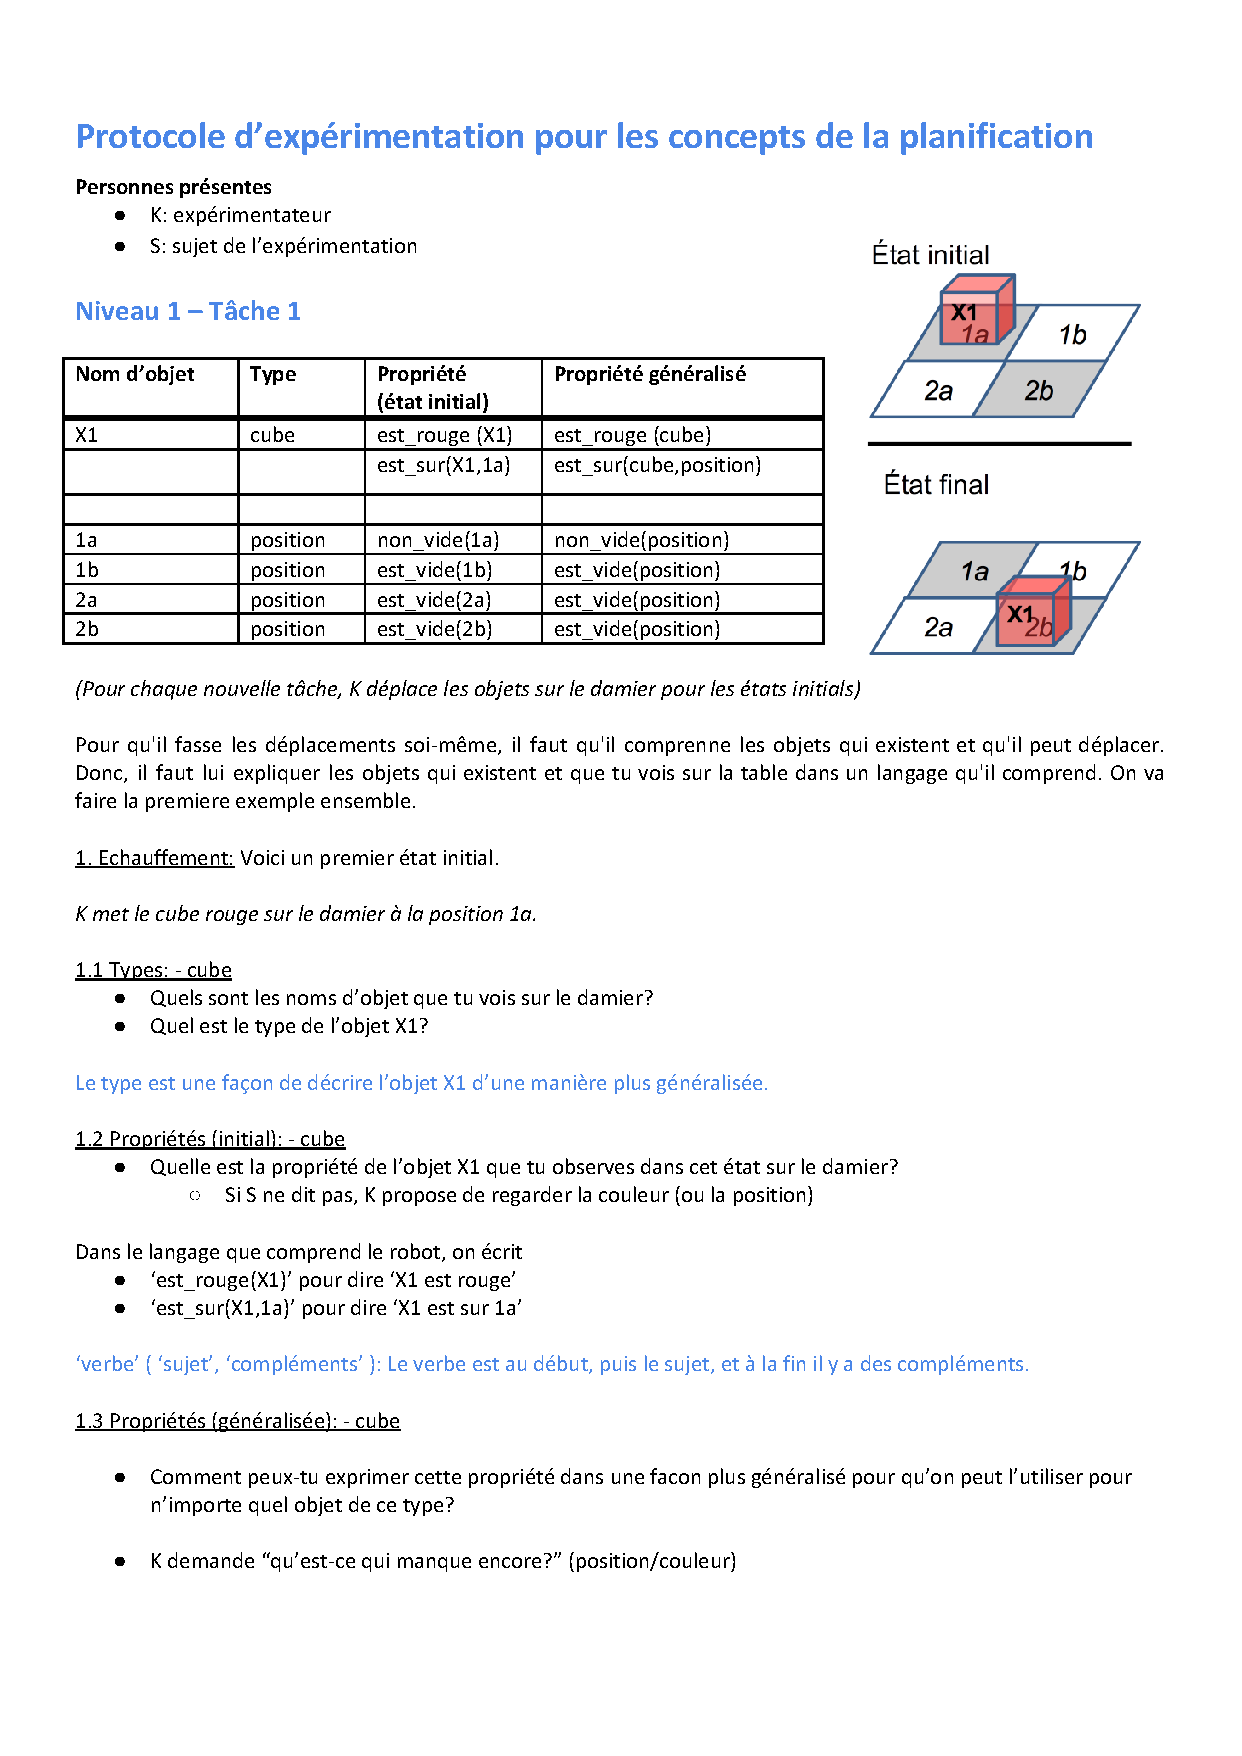
\includepdf[pages=1-6]{7-appendix/exp1-protocole.pdf}
%%\section{Questionnaire (In French)}
%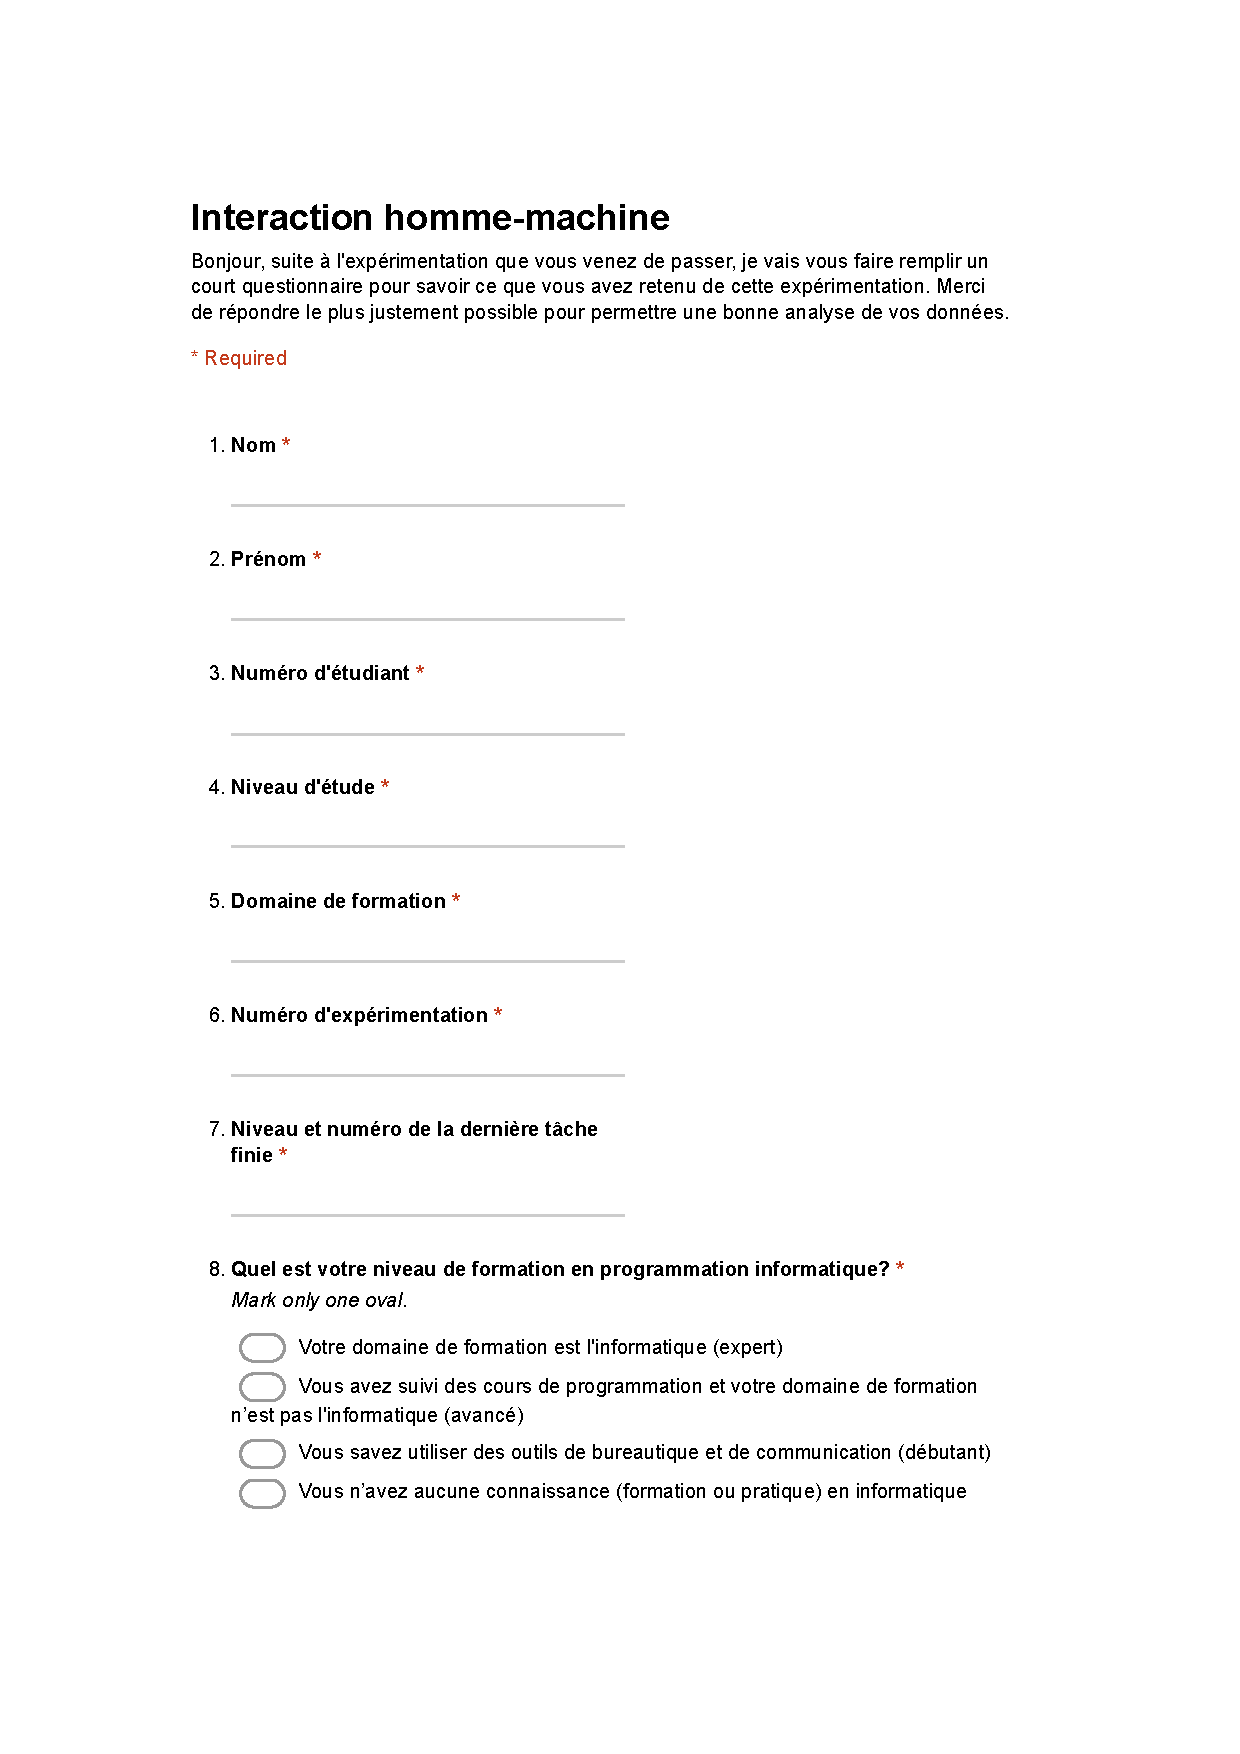
\includepdf[pages=1-7]{7-appendix/exp1-questionnaire.pdf}
%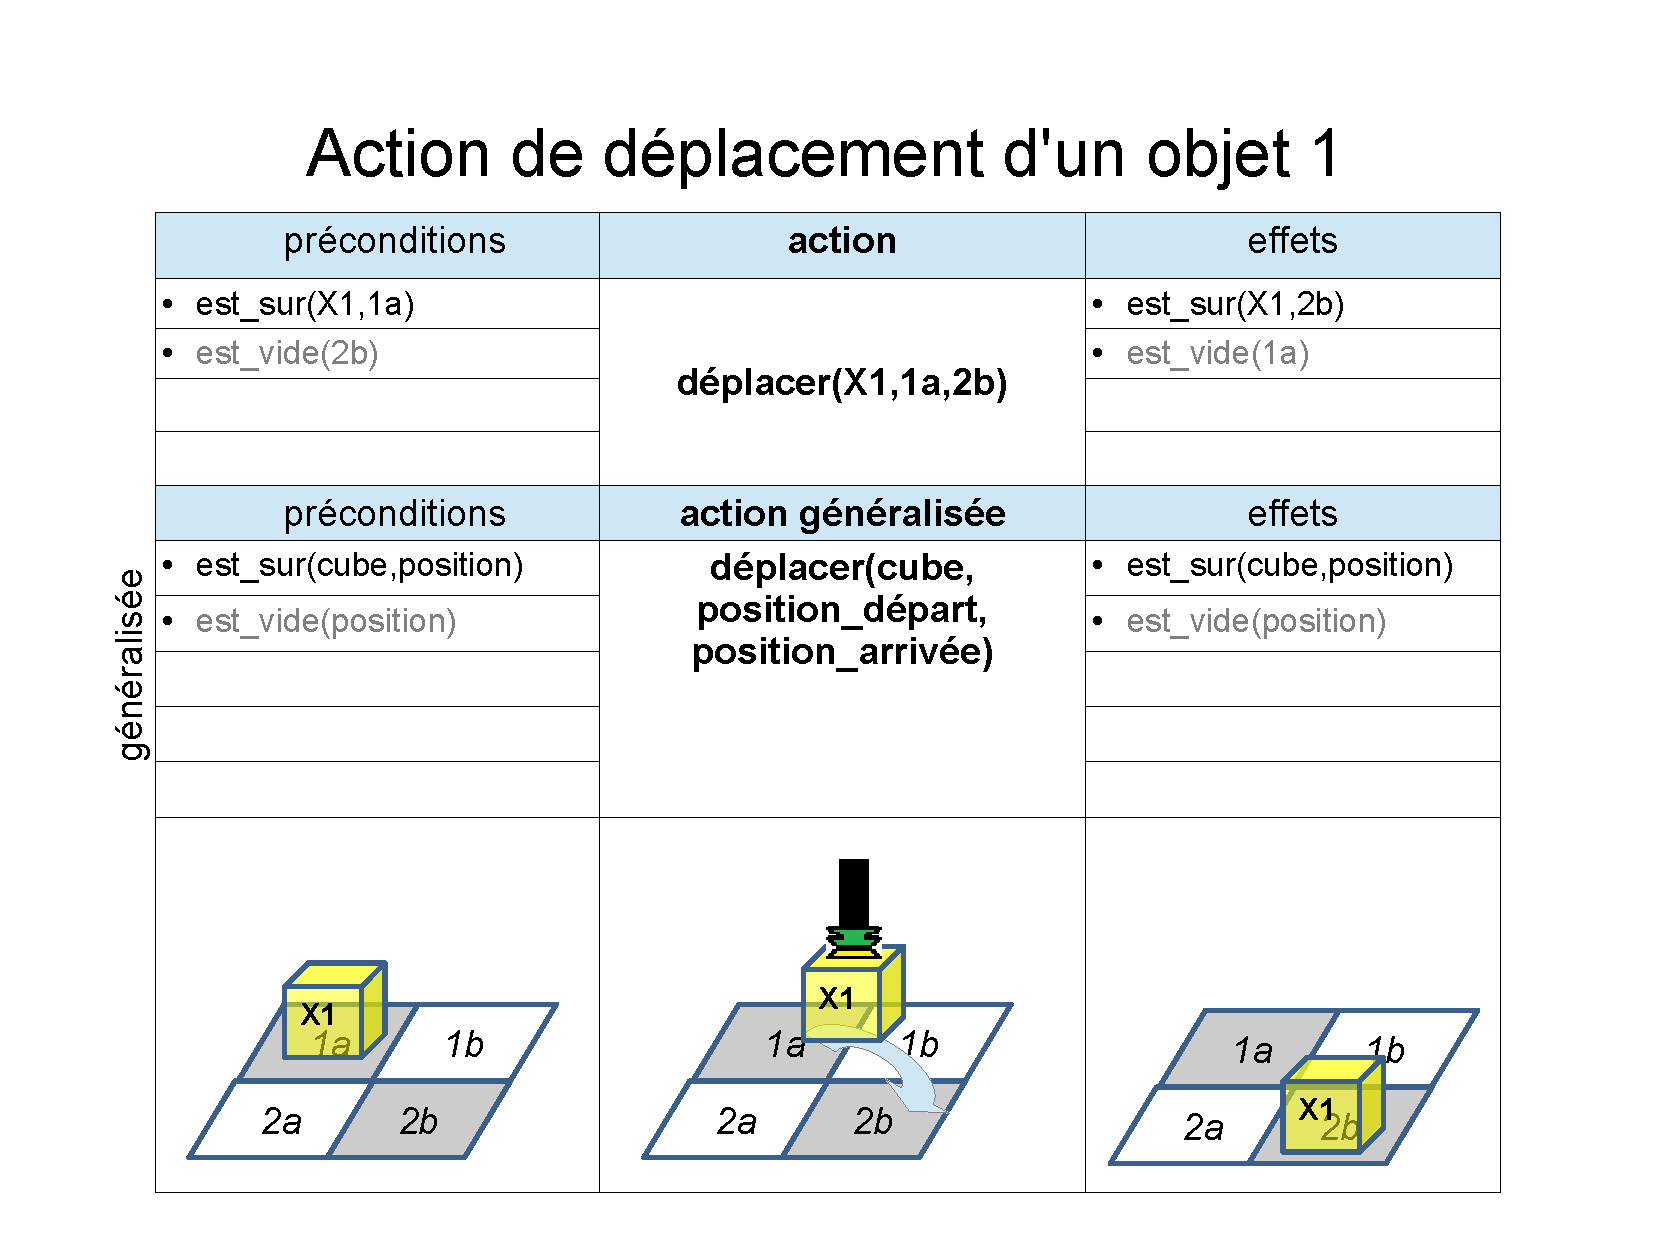
\includepdf[pages=1-4]{7-appendix/exp1-additionalmaterial.pdf}
%%\chapter{Notes during the experiments}
%%\includepdf[pages=1-5]{notes.pdf}

\chapter{Pre-Experiment 2 (\sect{sec:Exp2}): Protocol, Questionnaire and other Materials used}
\label{app:exp2}
A summary of the resources used for this section can be found online:
\begin{itemize}
	\item A demonstration of the Robot Programming process of our proposed framework: \url{https://youtu.be/DTm2YjiSNQM}
	\item GitHub repository of the system implemented for the Wizard-of-Oz technique: \url{https://github.com/ysl208/Baxter_PbD/}
\end{itemize}

%%\section{Experimental protocol (In French)}
%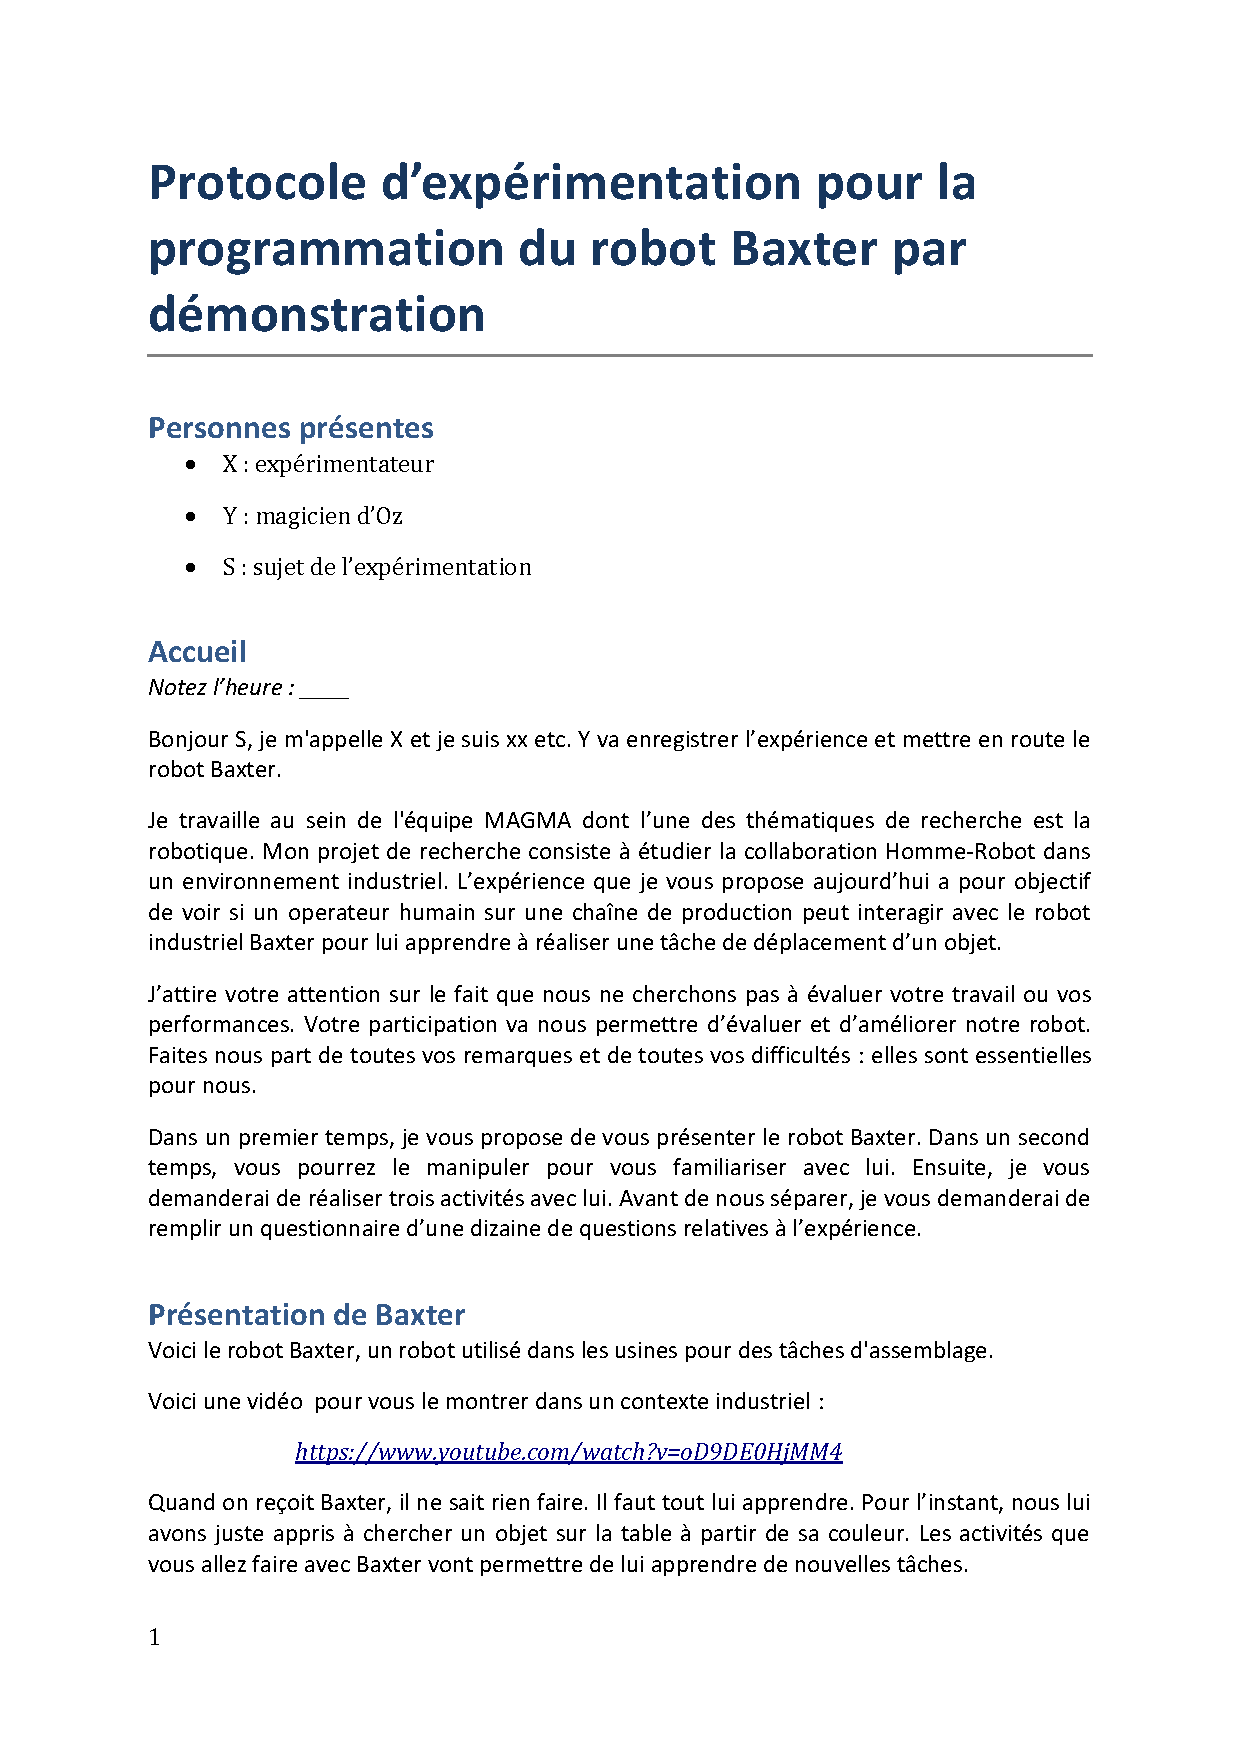
\includepdf[pages=1-7]{7-appendix/exp2-protocole.pdf}
%%\section{Questionnaire (In French)}
%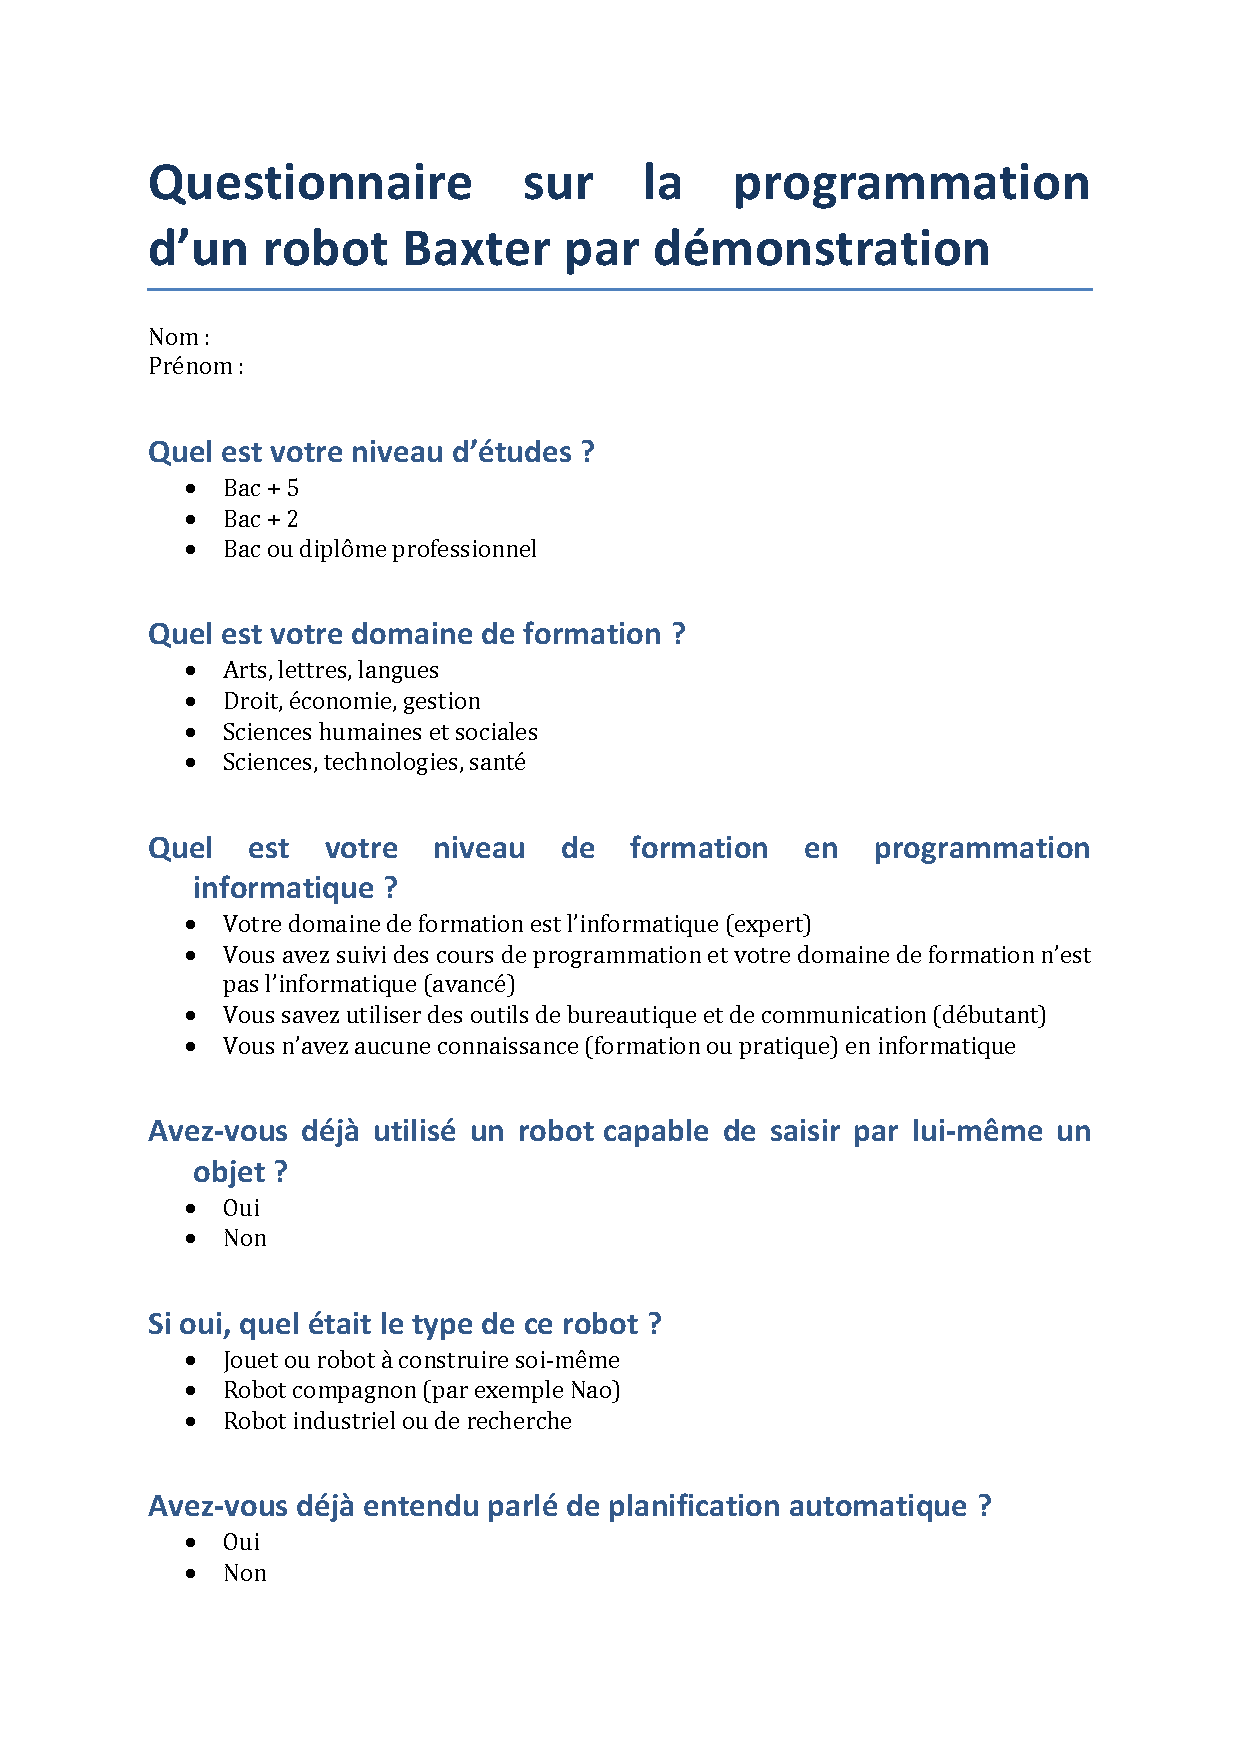
\includepdf[pages=1-3]{7-appendix/exp2-questionnaire.pdf}
%%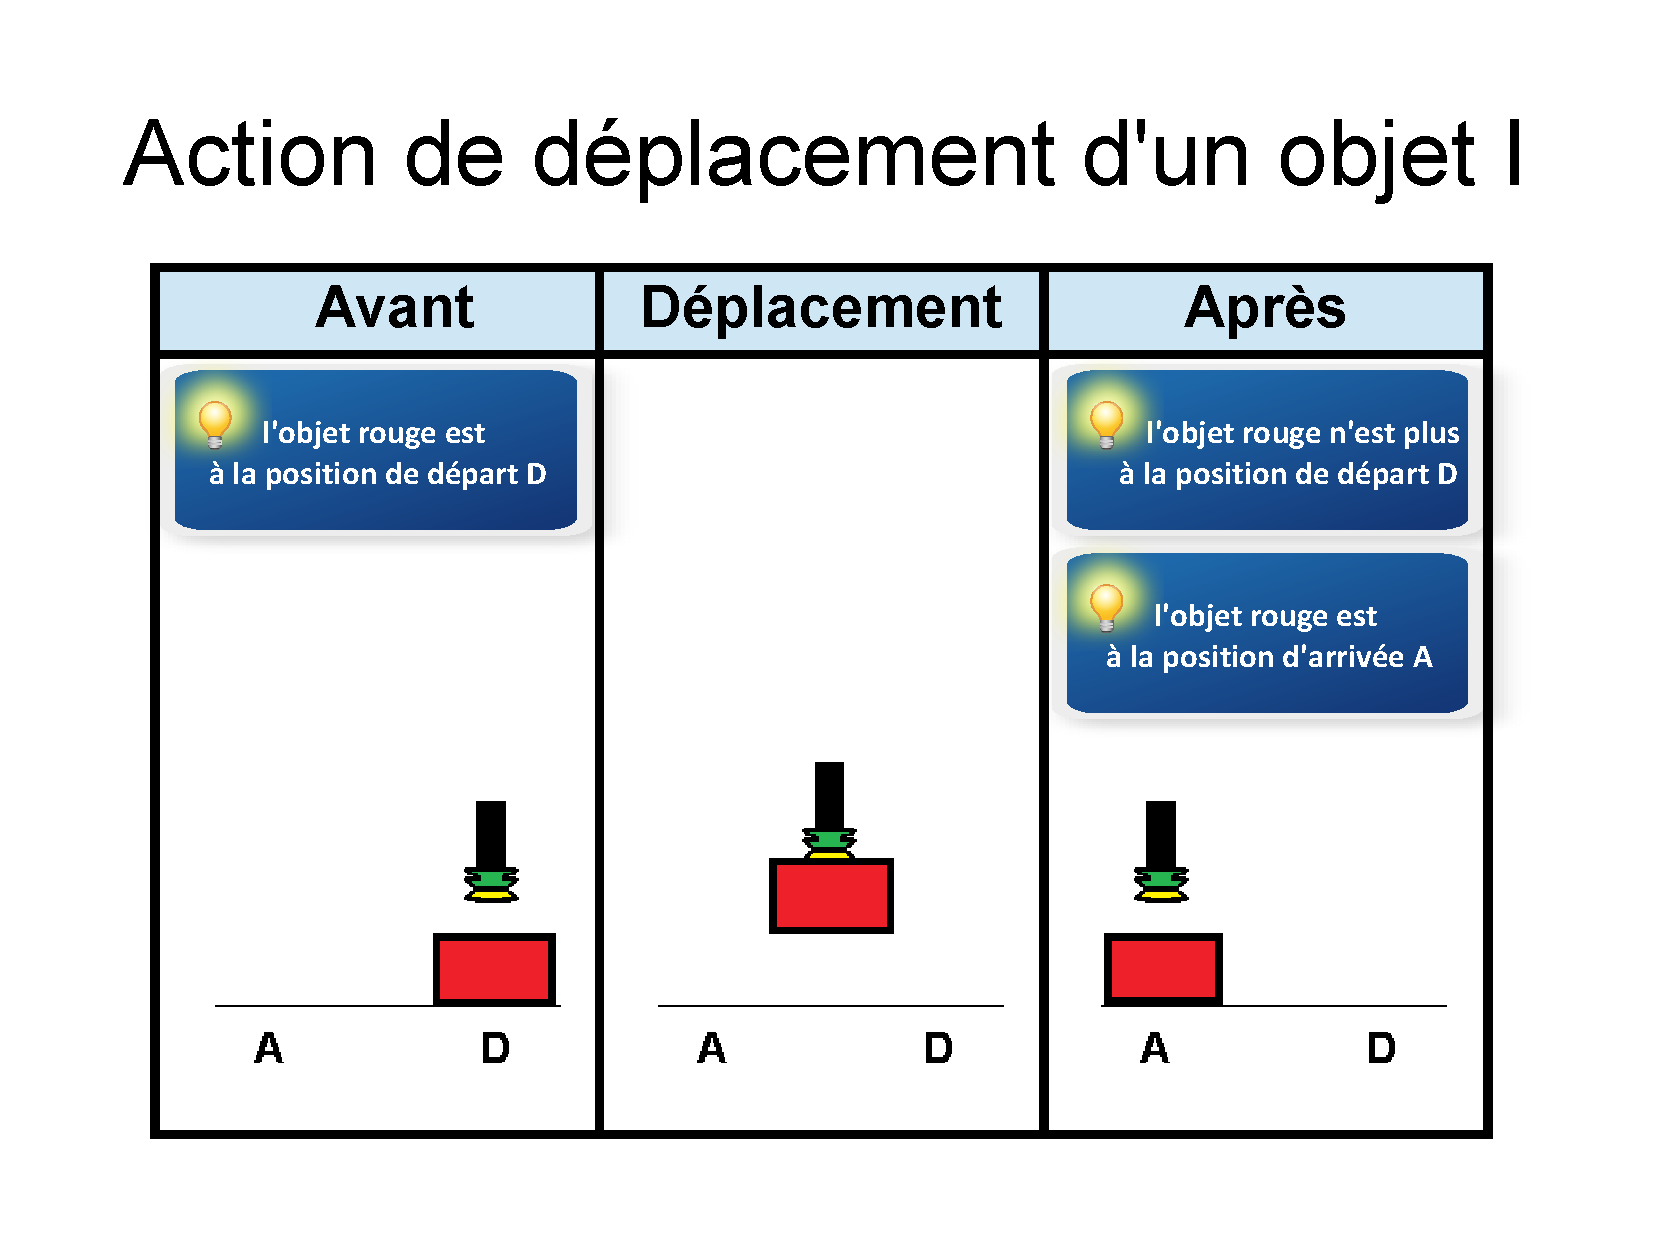
\includepdf[pages=1-3]{7-appendix/exp2-additionalmaterial.pdf}
%  \begin{figure}[h]
%    \centering
%    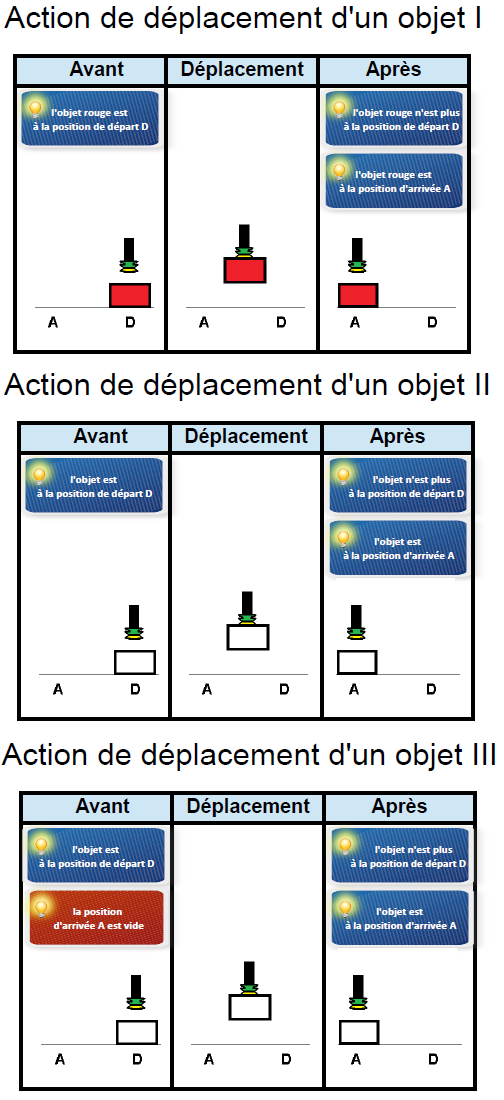
\includegraphics[scale=0.7]{figures/schema-all}
%    \caption{Action model used in experiments}
%    \label{fig:schema-all}
%  \end{figure}


\chapter{Experiment 3 (\chapt{chap:OrganisingTasks}): Protocol, Questionnaire and other Materials used}
\label{app:exp3}
A summary of the resources used for this section can be found online:
\begin{itemize}
	\item A demonstration of the Robot Programming process of our proposed framework: \url{https://youtu.be/liaSirH0CeM}
	\item Python code for simulating the teaching strategies: \url{https://github.com/ysl208/organisingtasks/}
	\item The graphical interface used for the AMT user study can be found on codepen:
	\url{https://codepen.io/ysliang208/project/editor/DYryzp#0}
\end{itemize}
%%\section{Experimental protocol}
%
\includepdf[pages=1-7]{7-appendix/exp3-protocole.pdf}
%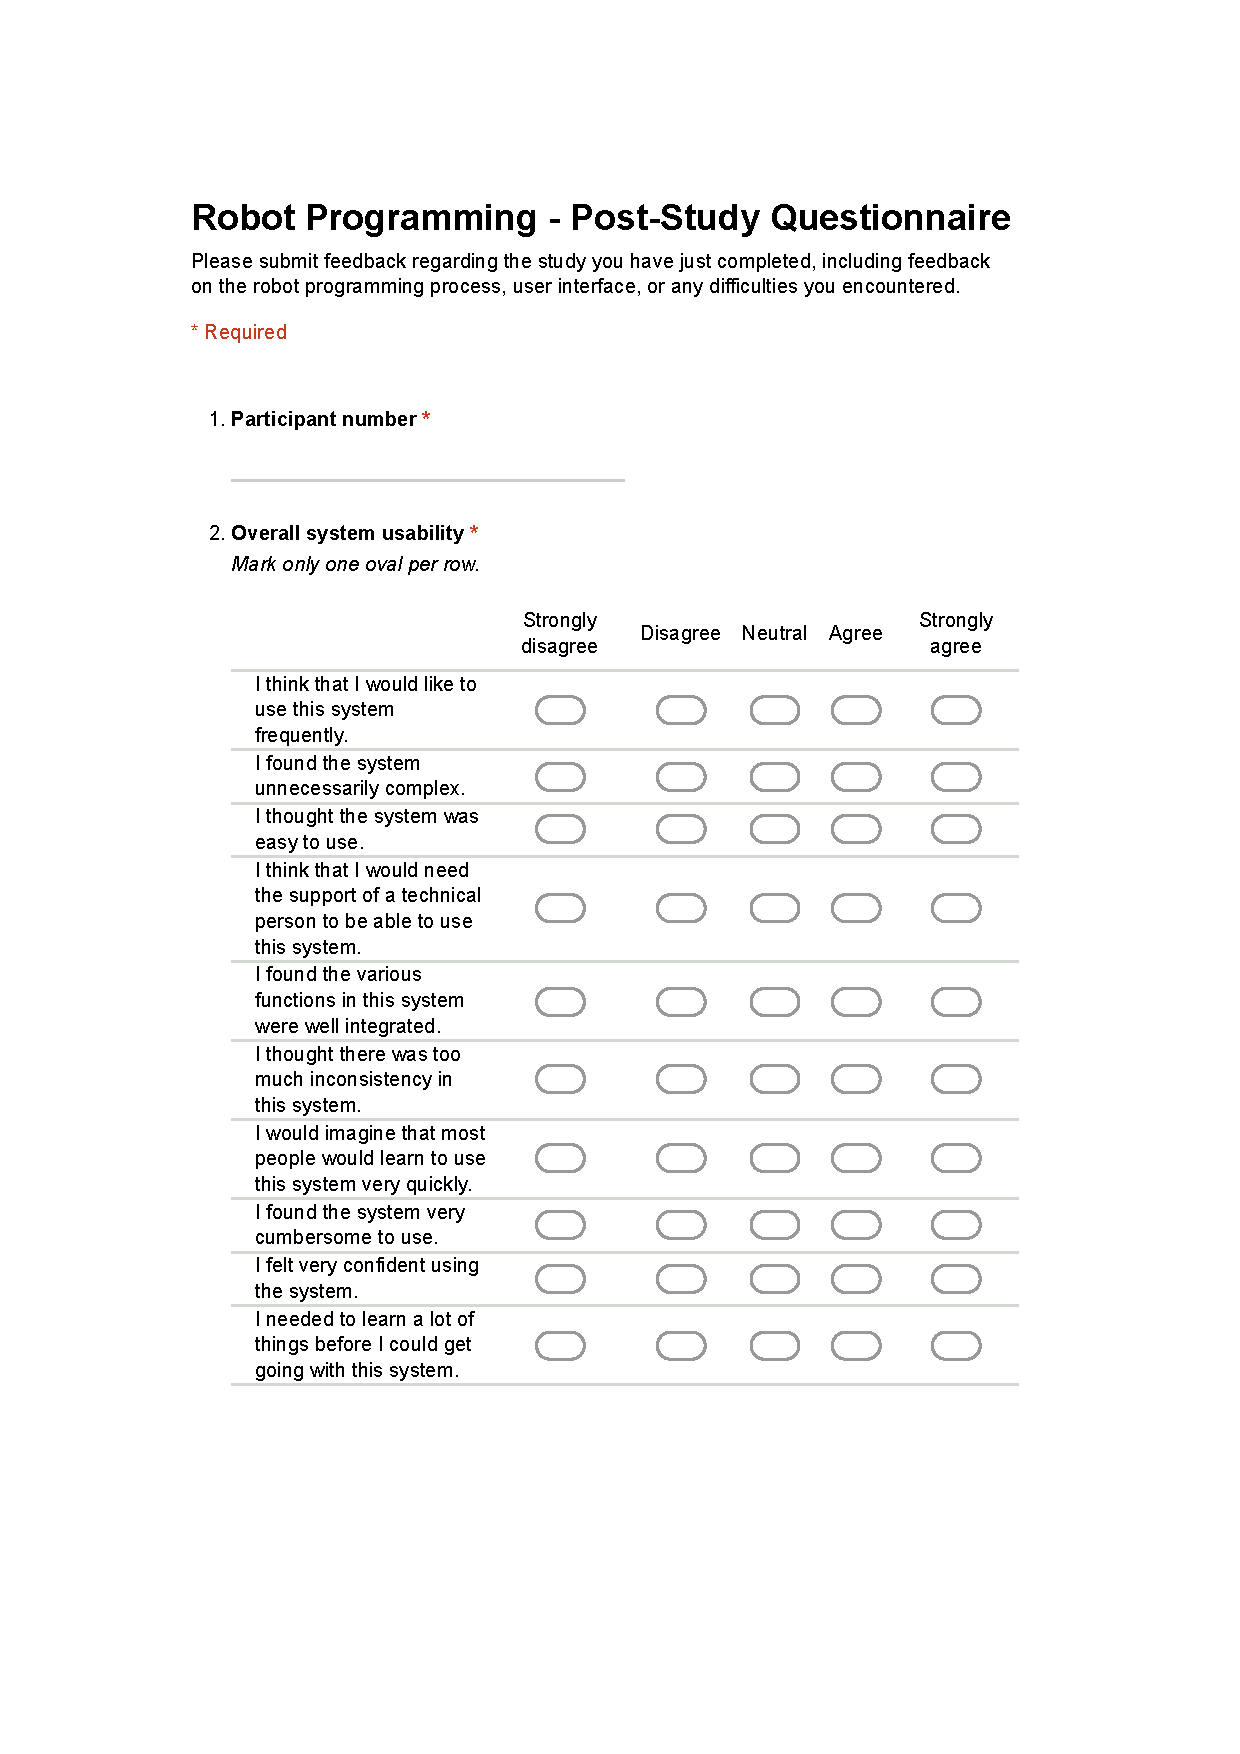
\includepdf[pages=1-3]{7-appendix/exp3-post-questionnaire.pdf}
%%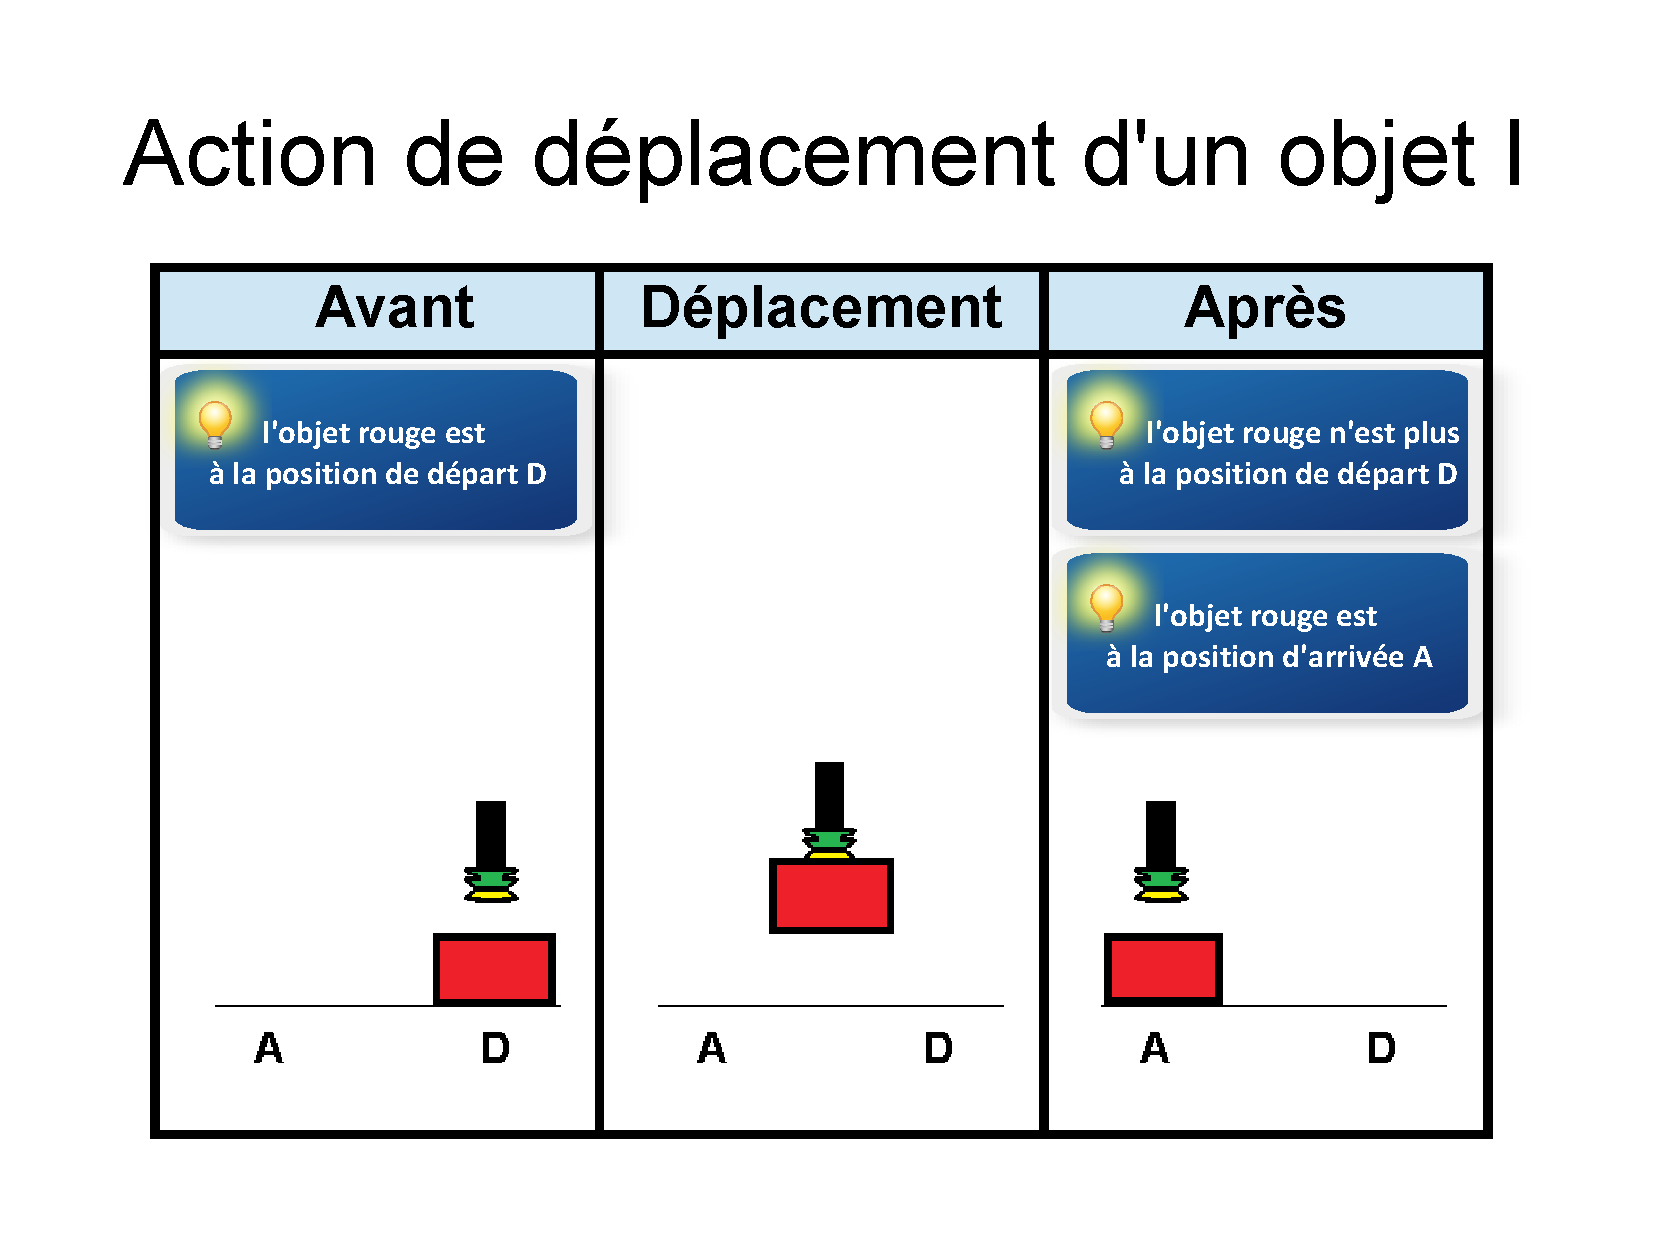
\includepdf[pages=1-3]{7-appendix/exp2-additionalmaterial.pdf}


\chapter{Experiment 4 (\sect{sec:quanteval}): Protocol, Questionnaire and other Materials used}
\label{app:exp4}
%%\section{Experimental protocol}
%
\includepdf[pages=1-7]{7-appendix/exp3-protocole.pdf}
%%\section{Questionnaire (In French)}
%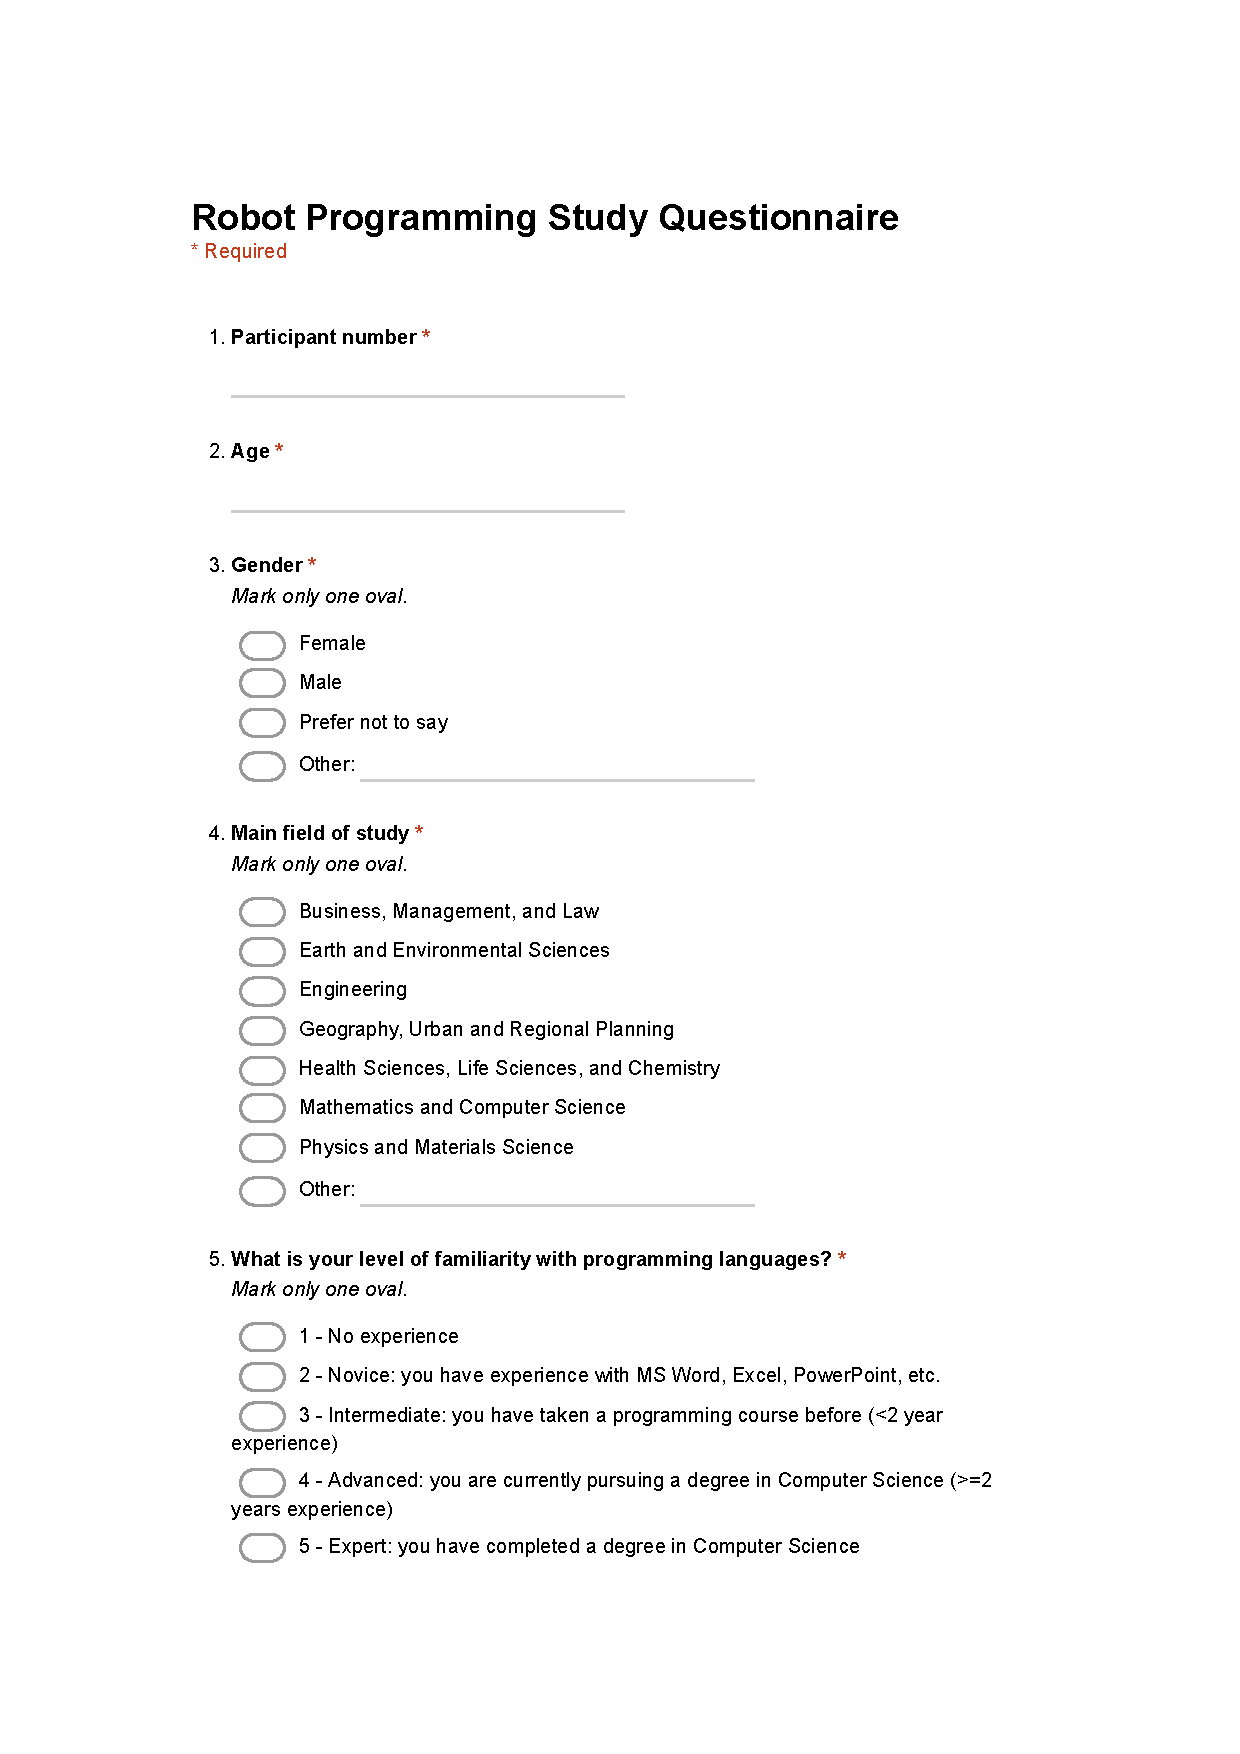
\includepdf[pages=1-3]{7-appendix/exp3-pre-questionnaire.pdf}
%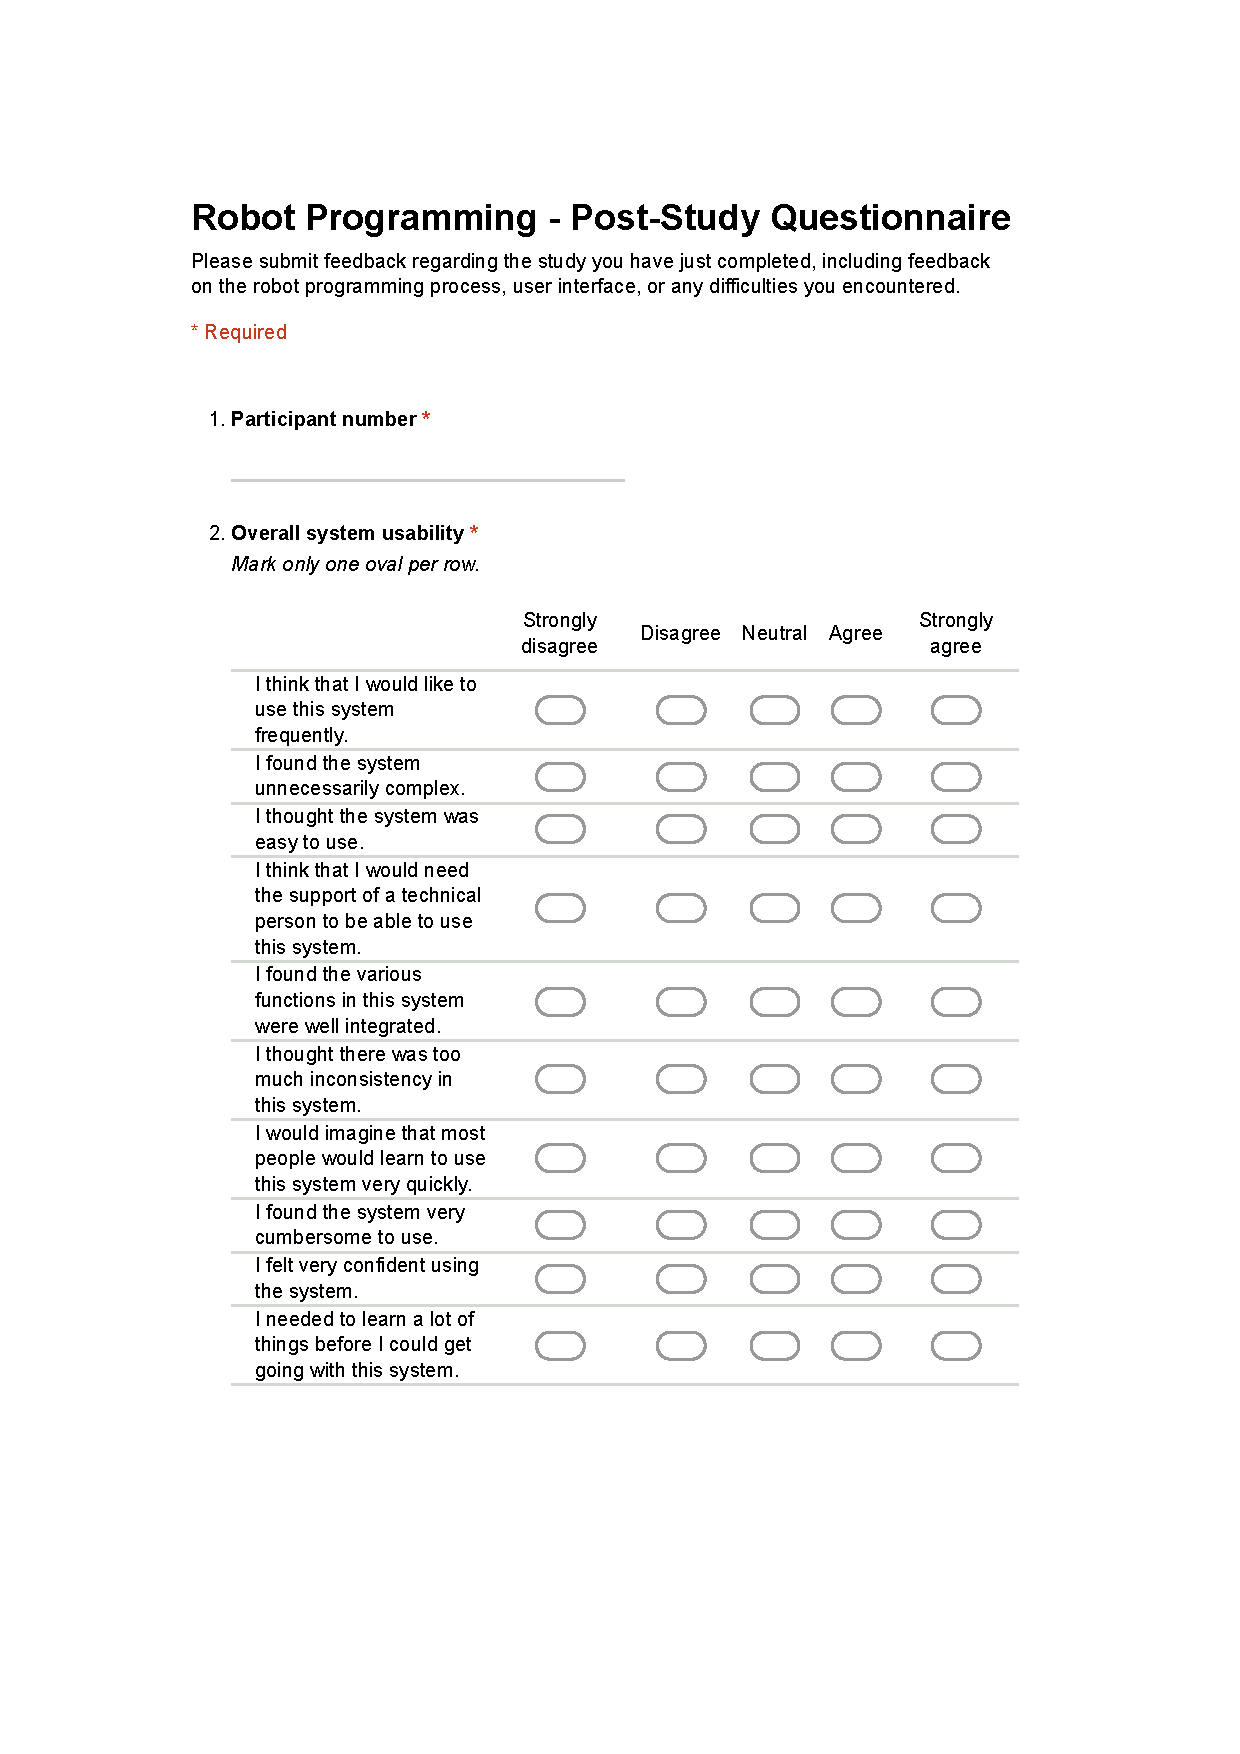
\includepdf[pages=1-3]{7-appendix/exp3-post-questionnaire.pdf}
%%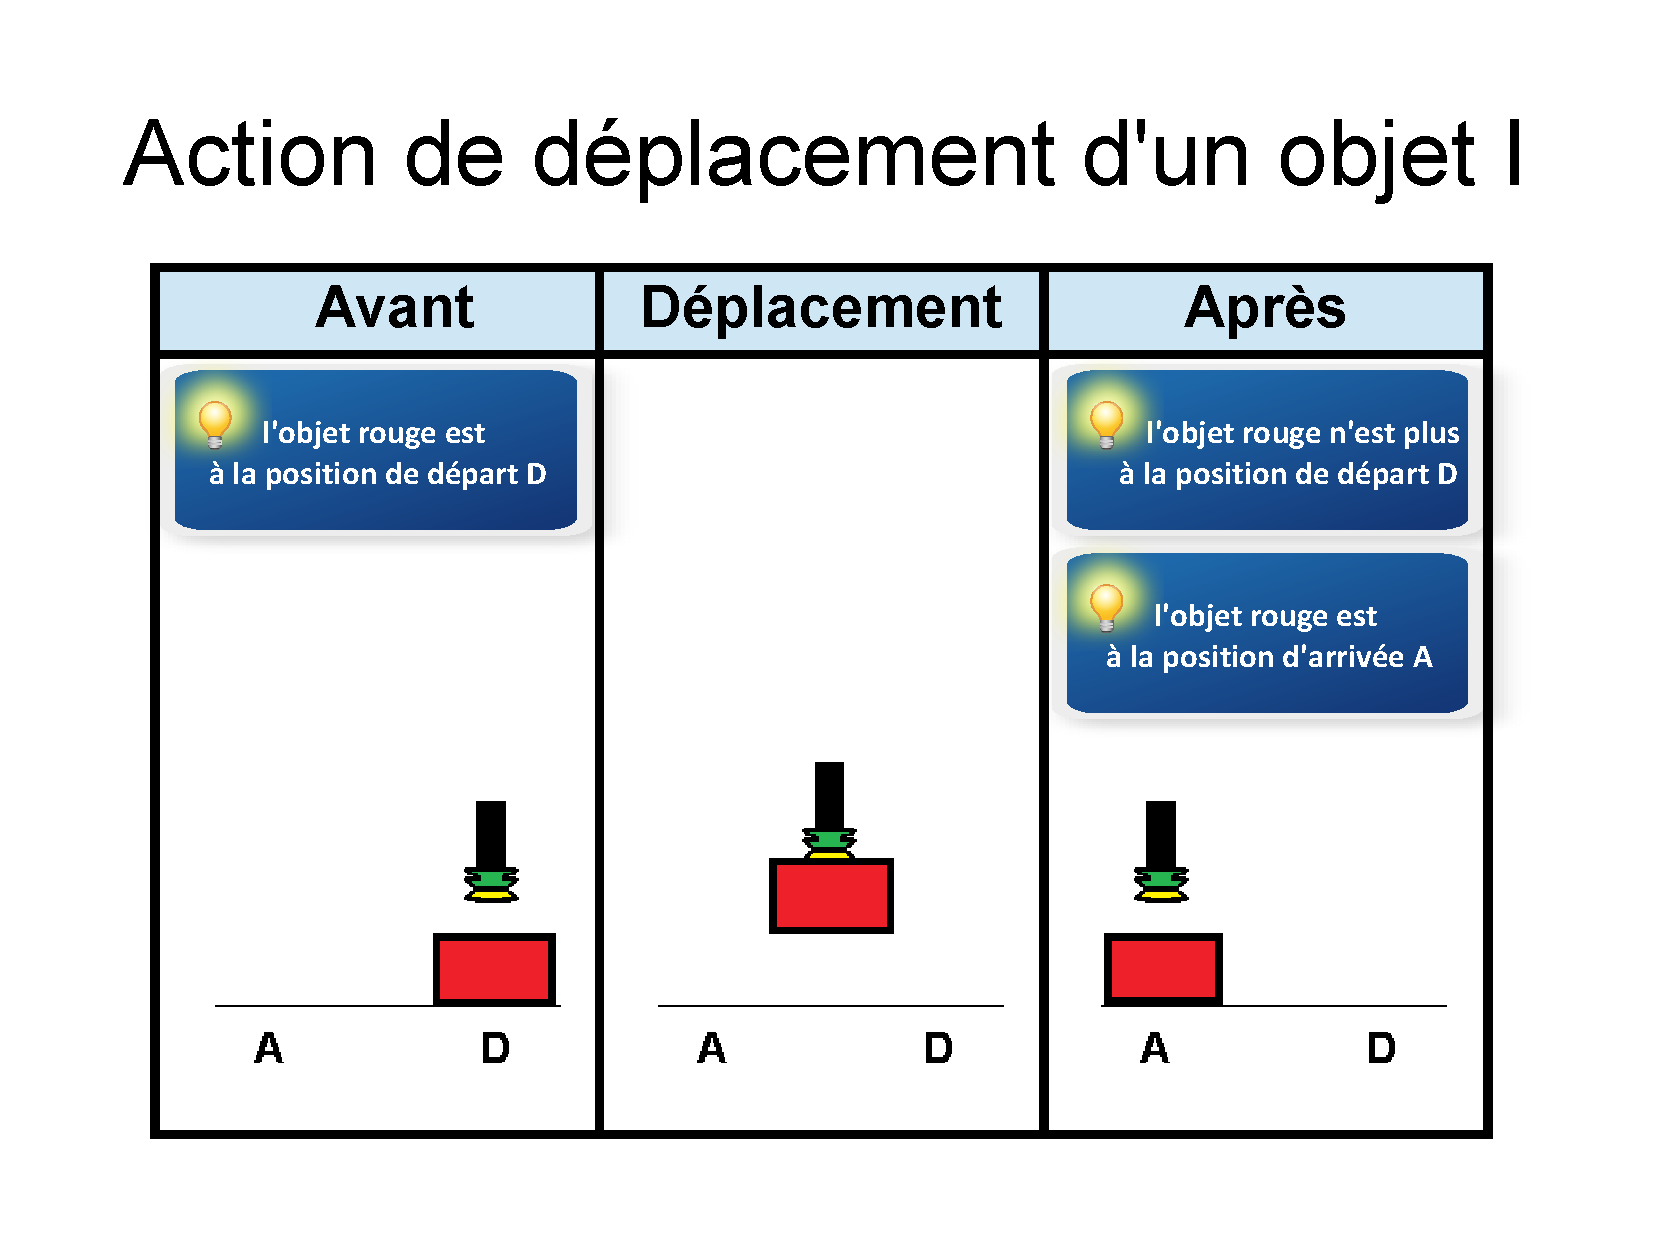
\includepdf[pages=1-3]{7-appendix/exp2-additionalmaterial.pdf}
%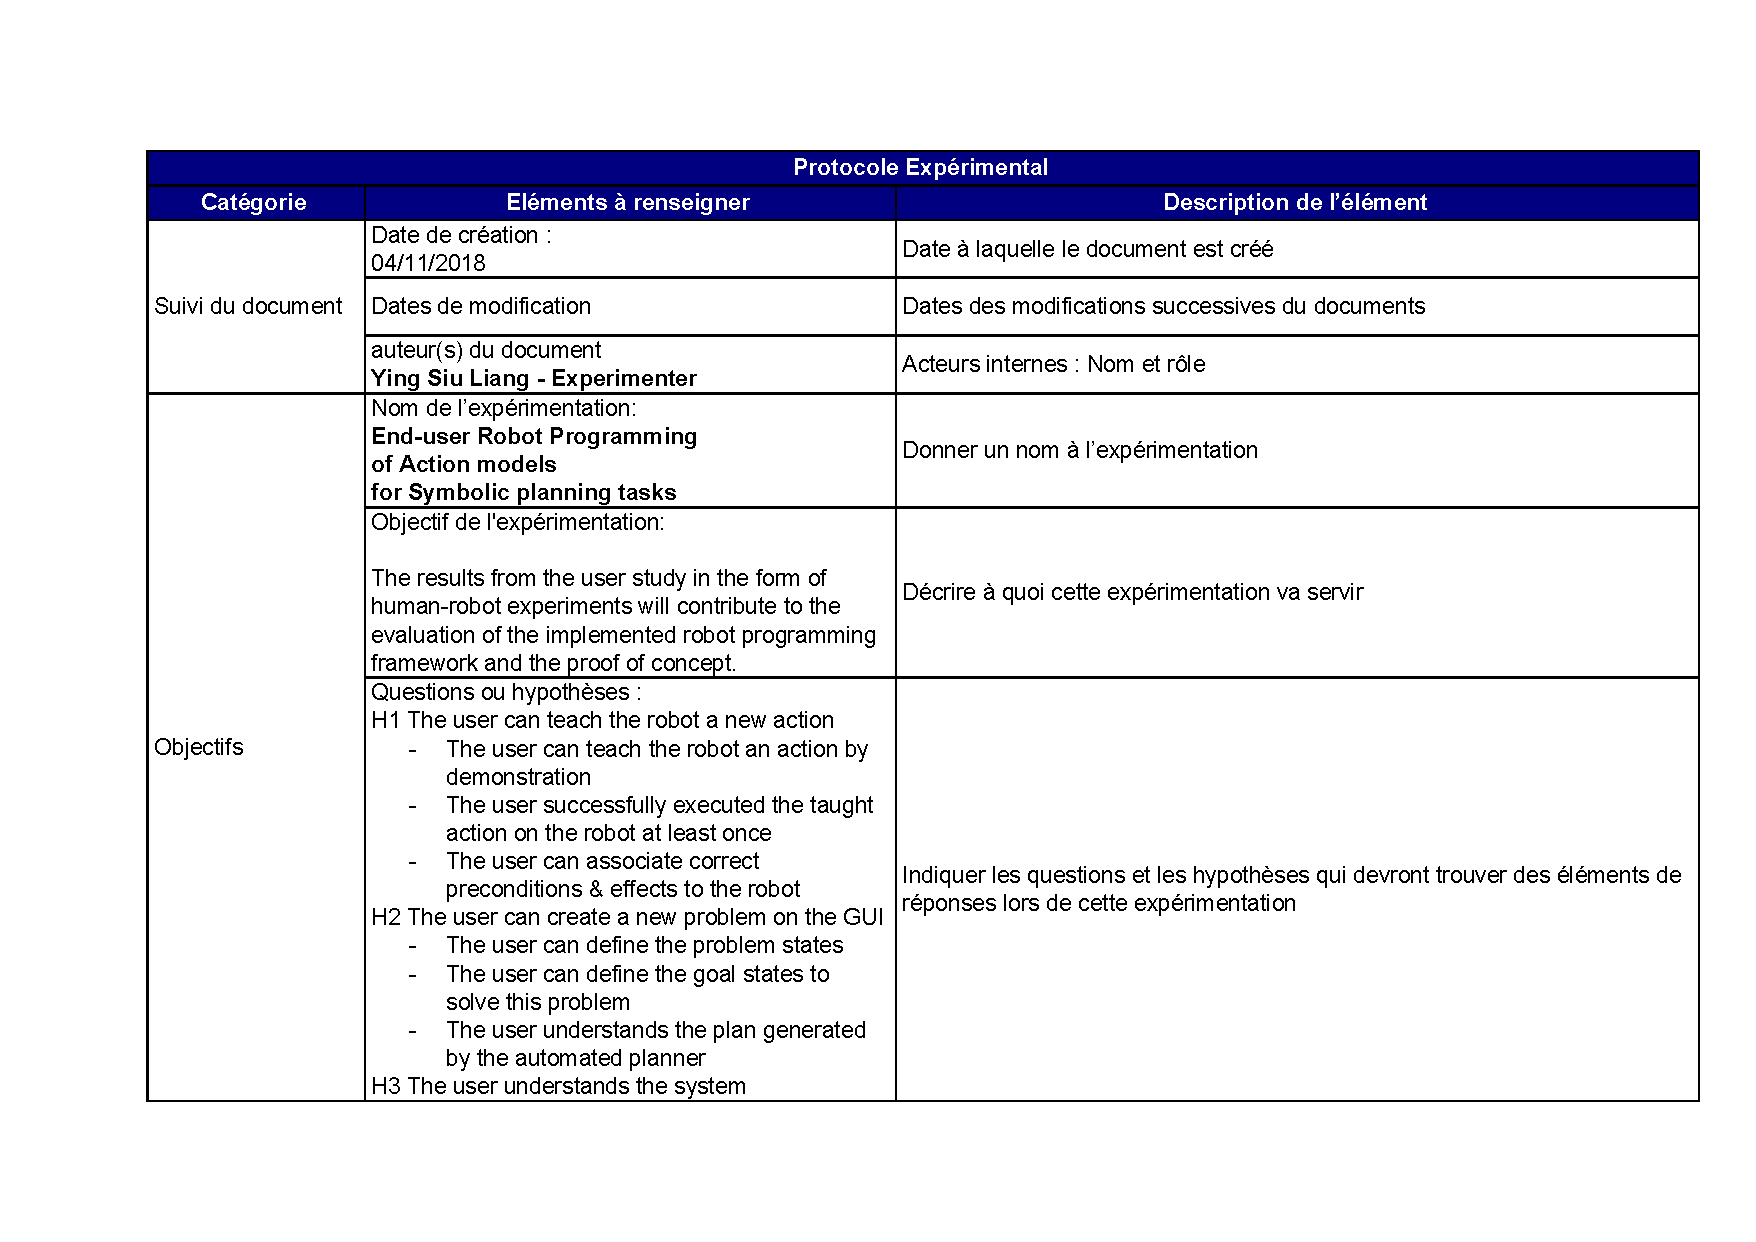
\includepdf[pages=1-4]{7-appendix/exp3-thedre-Guide-Protocole-Experimental.pdf}
%\includepdf[pages=1-3]{7-appendix/exp3-thedre-Guide-de-Brainstorming.pdf}

\chapter{PDDL code}\label{app:pddl}    
\section{iRoPro planning domain}
\begin{verbatim}
(define (domain iRoPro)
(:requirements :typing :strips)
(:types 
element 
position - element 
object - element 
cube - object 
base - object 
roof - object )

(:predicates
(clear ?obj - element)
(thin ?obj - element)
(flat ?obj - element)
(on ?obj2 - object ?obj1 - element)
(stackable ?obj2 - object ?obj1 - element) 
)

(:action move-vacuum
:parameters (?obj - object ?fromLoc - element ?toLoc - element )
:precondition (and (on ?obj ?fromLoc)
(clear ?toLoc)
(not(clear ?fromLoc))
(flat ?obj)
(stackable ?obj ?toLoc)
(clear ?obj) )
:effect (and (on ?obj ?toLoc)
(not(clear ?toLoc))
(clear ?fromLoc)
(not(on ?obj ?fromLoc)) )
)

(:action move-grip
:parameters (?obj - object ?fromLoc - element ?toLoc - element )
:precondition (and (on ?obj ?fromLoc)
(clear ?toLoc)
(not(clear ?fromLoc))
(thin ?obj)
(stackable ?obj ?toLoc)
(clear ?obj) )
:effect (and (on ?obj ?toLoc)
(not(clear ?toLoc))
(clear ?fromLoc)
(not(on ?obj ?fromLoc)) )
)

(:action side-pp
:parameters (?obj - object ?fromLoc - element ?toLoc - element )
:precondition (and (on ?obj ?fromLoc)
(clear ?toLoc)
(thin ?obj)
(stackable ?obj ?fromLoc)
(not(clear ?obj)) )
:effect (and (on ?obj ?toLoc)
(not(clear ?fromLoc))
(clear ?fromLoc)
(not(on ?obj ?fromLoc)) )
)
)
\end{verbatim}

\section{iRoPro planning problems}
\begin{verbatim}
(define (problem study-task3-swap)
(:domain iRoPro)
(:objects posA posB posC posM - position
obj1 obj2 - base)
(:init (clear obj1) (on obj1 posA) (clear obj2) (on obj2 posB) 
(clear posC) (not(clear posB)) (not(clear posA)) (clear posM) 
(stackable obj1 obj2) (stackable obj1 posA) (stackable obj1 posB) 
(stackable obj1 posC) (stackable obj1 posM) (flat obj1) 
(stackable obj2 obj1) (stackable obj2 posA) (stackable obj2 posB) 
(stackable obj2 posC) (stackable obj2 posM) (flat obj2) 
(flat posA) (flat posB) (flat posC) (flat posM))
(:goal (on obj1 posB) (on obj2 posA) )
)

(define (problem blocksworld-task2)
(:domain iRoPro)
(:objects posA posB posC posD posE posM - position
obj1 - base
obj2 obj3 obj4 - roof)
(:init (clear obj1) (on obj1 posB) (clear obj2) (on obj2 posM) 
(clear obj3) (on obj3 posC) (clear obj4) (on obj4 posE) 
(not(clear posC)) (not(clear posM)) (clear posA) (not(clear posB))
(clear posD) (not(clear posE)) (stackable obj1 posA) 
(stackable obj1 posB) (stackable obj1 posC) (stackable obj1 posD) 
(stackable obj1 posE) (stackable obj1 posM) (flat obj1) 
(stackable obj2 obj1) (stackable obj2 posA) (stackable obj2 posB) 
(stackable obj2 posC) (stackable obj2 posD) (stackable obj2 posE) 
(stackable obj2 posM) (thin obj2) (stackable obj3 obj1) 
(stackable obj3 posA) (stackable obj3 posB) (stackable obj3 posC) 
(stackable obj3 posD) (stackable obj3 posE) (stackable obj3 posM) 
(thin obj3) (stackable obj4 obj1) (stackable obj4 posA) 
(stackable obj4 posB) (stackable obj4 posC) (stackable obj4 posD) 
(stackable obj4 posE) (stackable obj4 posM) (thin obj4) (flat posA) 
(flat posB) (flat posC) (flat posD) (flat posE) (flat posM))
(:goal (and (on obj1 posM) (on obj3 obj1) (on obj4 obj3) (on obj2 obj4) 
)))

(define (problem blocksworld-task34)
(:domain iRoPro)
(:objects posA posB posC posD posE posM - position
obj1 obj2 obj3 obj4 - roof)
(:init (clear obj4) (clear posC) (clear posB) (clear posE) 
(on obj1 obj2) (on obj3 obj1) (on obj4 obj3) (on obj2 posM) 
(stackable obj1 posA) (stackable obj1 posB) (stackable obj1 posC) 
(stackable obj1 posD) (stackable obj1 posE) (stackable obj1 posM) 
(thin obj1) (stackable obj2 posA) (stackable obj2 posB) 
(stackable obj2 posC) (stackable obj2 posD) (stackable obj2 posE) 
(stackable obj2 posM) (thin obj2) (stackable obj3 posA) 
(stackable obj3 posB) (stackable obj3 posC) (stackable obj3 posD) 
(stackable obj3 posE) (stackable obj3 posM) (thin obj3) 
(stackable obj4 posA) (stackable obj4 posB) (stackable obj4 posC) 
(stackable obj4 posD) (stackable obj4 posE) (stackable obj4 posM) 
(thin obj4) (flat posA) (flat posB) (flat posC) (flat posD) (flat posE) 
(flat posM))
(:goal (and (on obj1 obj2) (on obj3 obj1) (on obj4 obj3) (on obj2 posB) 
)))

\end{verbatim}


\end{document}